%\chapter{Generalized Spherical Harmonics}
\chapter{广义球谐函数}
\label{chapter:gsh}

我们当然期望有一个能够将附录B中所讨论的标量和矢量球谐函数展开拓展到更高阶张量场的方法。
\index{vector spherical harmonics}%
\index{spherical harmonics!vector}%
Backus (\citeyear{backus67})发展了一种势函数表示,将二阶切向张量场 $\bT^{\Omega\Omega}$用四个标量场表示,类似于切向矢量场两个势函数表示
$\bu^{\Omega}=\bdel_1V-\brh\times\bdel_1W$,并用其简洁地推导了球对称地球模型的环型和球型自由振荡所满足的径向微分方程,还得到了地幔中可能的初始静态应力场的详尽结果。
他的表述方法可以与切向矢量及张量分解$\bT=\brh\brh T_{rr}
+\brh\bT^{r\Omega}+\bT^{\Omega r}\brh+\bT^{\Omega\Omega}$结合使用,
来定义九个二阶张量球谐函数,类似于三个矢量球谐函数$\bP_{lm}$、$\bB_{lm}$、 $\bC_{lm}$。然而,该方法植根于经典微分几何,很难推广到更高阶张量$\bT$。

\enlargethispage{-0.5\baselineskip}
在本附录中,我们介绍一个更有效同时也是更常规的方法,将
任意阶数的张量场用{\em 广义球谐函数\/}展开。
\index{generalized spherical harmonics}%
\index{spherical harmonics!generalized}%
Gelfand \& Shapiro
(\citeyear{gelfand&shapiro56})首次将广义球谐函数展开系统地应用于求解经
典张量微分方程。他们的结果被Burridge (\citeyear{burridge69}) 加以凝练并置于实用的基础上,随后Phinney \& Burridge (\citeyear{phinney&burridge73})将其应用于地球自由振荡的研究。广义球谐函数和旋转群$O(3)$表述之间有密切的联系; 然而,我们在此不会将精力花在这些理论细节上。我们有一个具体且更有限的目标:发展一套数学系统来处理涉及球极坐标中的矢量和更高阶张量的代数和微分关系式。一旦掌握了几个基本概念,就能够使用该系统\textcolor{red}{随心所欲地}进行广义球谐函数计算,而不用考虑分析中的群论支撑。
%%%
在继续之前,需要谨慎地指出本附录中所描述的广义矢量球谐函数{\em 并不是\/}电场和磁场之间相互作用的量子理论研究中常用的矢量球谐函数(Edmonds \citeyear{edmonds60})。
后者是用由三个复数笛卡尔矢量$-\frac{1}{\sqrt{2}}(\bxh+i\byh)$、$\bzh$、\vspace{-0.4 mm}
$\frac{1}{\sqrt{2}}(\bxh-i\byh)$所构成的一组基展开的,而Gelfand-Shapiro-Burridge球谐函数则是以我们在附录~\ref{C.sec.twobases}中所定义的正则球极基矢量
$\beh_-$、$\beh_0$、$\beh_+$和$\beh^-$、$\beh^0$、
$\beh^+$表示的。
量子电磁矢量球谐函数的表达被置于严格的经典框架内,并由James (\citeyear{james76})扩展至任意阶的张量;
他的极富可读性的论文为该题目提供了一个全面介绍。然而,我们在本书中不去讨论Edmonds-James张量球谐函数的特性,因为由于历史的原因,它从未被用于理论全球地震学。

通过与(\ref{B.inprod})类比,我们定义单位球$\Omega$上两个(不一定是切向)张量场$\bT$和
$\bP$的{\em 内积\/}为
\index{inner product!of tensor fields}%
\eq
\label{C.inprod}
\langle\bT,\bP\rangle=\int_\Omega \bT^*\hspace{-0.2 mm}\tdot\bP\,d\Om.
\en
其中三重点积表示对所有球极分量的缩并:
$\bT^*\hspace{-0.2 mm}\tdot\bP=T^*_{rr\cdots r}P_{rr\cdots r}+
T^*_{\theta r\cdots r}P_{\theta r\cdots r}+\cdots
T^*_{\phi\phi\cdots\phi}P_{\phi\phi\cdots\phi}$.
对于单位球面上的两个张量场$\bT$和$\bP$,如果有 $\langle\bT,\bP\rangle=0$,则称它们是{\em 正交的\/}。由内积~(\ref{C.inprod}) 产生的张量{\em 范数\/}用
$\|\hspace{-0.3 mm}|\hspace{0.2 mm}\bT\hspace{0.2 mm}\|\hspace{-0.3 mm}|
=\langle\bT,\bT\rangle^{1/2}$表示。用三条竖线是为了要与复数的欧氏范数 $\|\bT\|=(\bT^*\tdot\bT)^{1/2}$有所区别。

%\section{Angular Momentum---Reprise}
\section{角动量回顾}
\index{angular momentum|(}%
\label{section:rotations}

我们首先考虑在附录B.2中引入的角动量算子$\bL$的一个至此尚未提及的性质。
我们将看到,$\bL$自然地出现在刚体旋转下标量场变换特性的分析中;
然而,如果我们试图也用它来描述矢量和更高阶的张量场的变换特性,则 必须将其加以推广。从一个不带撇的笛卡尔坐标系$\bxh$、$\byh$、$\bzh$ 到一个带撇的笛卡尔坐标系$\bxh'$、$\byh'$、$\bzh'$的刚性旋转可以用如下矩阵描述:
\eq \label{C.Rdef}
\ssR=\left(\begin{array}{ccc}
\bxh'\cdot\bxh \hspace{1.0 mm} & \byh'\cdot\bxh \hspace{1.0 mm} & \bzh'\cdot\bxh \\
\vspace{-0.4 ex} & \vspace{-0.4 ex} & \vspace{-0.4 ex} \\
\bxh'\cdot\byh \hspace{1.0 mm} & \byh'\cdot\byh \hspace{1.0 mm} & \bzh'\cdot\byh \\
\vspace{-0.4 ex} & \vspace{-0.4 ex} & \vspace{-0.4 ex} \\
\bxh'\cdot\bzh \hspace{1.0 mm} & \byh'\cdot\bzh \hspace{1.0 mm} & \bzh'\cdot\bzh
\end{array}\right).
\en
所有由方向余弦组成的这种矩阵都是正当正交的:$\ssR^{-1}=\ssR^{\rm T}$和${\rm det}\,\ssR=1$。单位球$\Omega$上一点的带撇和不带撇坐标$\brh=x\bxh+y\byh+z\bzh
=x'\hat{\bf x}'+y'\hat{\bf y}'+z'\hat{\bf z}'$之间的关系为
\eq \label{C.Rdef2}
\left(\begin{array}{c}
x' \\ \vspace{-1.0 ex} \\ y' \\ \vspace{-1.0 ex} \\ z'
\end{array}\right)=\ssR
\left(\begin{array}{c}
x \\ \vspace{-1.0 ex} \\ y \\ \vspace{-1.0 ex} \\ z
\end{array}\right).
\en
欧拉定理断言,每一正当正交的矩阵$\ssR$都与一矢量 $\bomega$同构,该矢量的方向$\hat{\bomega}$为旋转轴,其长度$\|\bomega\|$ 为以弧度为单位的右手旋转角。
逆矩阵或转置矩阵$\ssR^{-1}=\ssR^{\rm T}$与矢量$-\bomega$相对应,而单位矩阵$\ssI$ 则与零矢量相对应。

需要强调的是,(\ref{C.Rdef2})式中的$x'$、$y'$、$z'$和$x$、$y$、$z$
是{\em 同一点\/}$\brh$在两个笛卡尔系统中的坐标。这种{\em 被动\/}的观点在地球物理应用中是最方便的,
\index{rigid rotation!passive}%
\index{rotation!rigid}%
\index{rotation!passive}%
\index{passive rotation}%
也是我们在此唯一采用的;{\em 主动\/}的观点是保持正交归一轴$\bxh$、$\byh$、 $\bzh$固定,而观察点$\brh=x\bxh+y\byh+z\bzh$移动到 $\brh'=x'\bxh+y'\byh+z'\bzh$,常常在量子力学中用来描述物理系统的旋转对波函数的影响 (Schiff \citeyear{schiff68})。如图~\ref{C.fig.passrot}所示,一个围绕单一固
定轴的被动旋转$\bomega$与一个等量且反向的主动旋转$-\bomega$是等效的。

从$\bxh$、$\byh$、$\bzh$到$\bxh'$、$\byh'$、$\bzh'$的旋转$\ssR_1$和随后从$\bxh'$、 $\byh'$、$\bzh'$到$\bxh''$、$\byh''$、 $\bzh''$的旋转$\ssR_2$这两个接续旋转的净效果可以表述为
\eq \label{C.R1R2def}
\left(\begin{array}{c}
x'' \\ \vspace{-1.0 ex} \\ y'' \\ \vspace{-1.0 ex} \\ z''
\end{array}\right)=\ssR_2\ssR_1
\left(\begin{array}{c}
x \\ \vspace{-1.0 ex} \\ y \\ \vspace{-1.0 ex} \\ z
\end{array}\right),
\en
其中
\eqa \label{C.R1R2def2} \lefteqn{
\ssR_2\ssR_1=\left(\begin{array}{ccc}
\bxh''\cdot\bxh' \hspace{1.0 mm} & \byh''\cdot\bxh' \hspace{1.0 mm}
& \bzh''\cdot\bxh' \\
\vspace{-0.4 ex} & \vspace{-0.4 ex} & \vspace{-0.4 ex} \\
\bxh''\cdot\byh' \hspace{1.0 mm} & \byh''\cdot\byh' \hspace{1.0 mm} &
\bzh''\cdot\byh' \\
\vspace{-0.4 ex} & \vspace{-0.4 ex} & \vspace{-0.4 ex} \\
\bxh''\cdot\bzh' \hspace{1.0 mm} & \byh''\cdot\bzh' \hspace{1.0 mm} &
\bzh''\cdot\bzh'
\end{array}\right)\left(\begin{array}{ccc}
\bxh'\cdot\bxh \hspace{1.0 mm} & \byh'\cdot\bxh \hspace{1.0 mm} & \bzh'\cdot\bxh \\
\vspace{-0.4 ex} & \vspace{-0.4 ex} & \vspace{-0.4 ex} \\
\bxh'\cdot\byh \hspace{1.0 mm} & \byh'\cdot\byh \hspace{1.0 mm} & \bzh'\cdot\byh \\
\vspace{-0.4 ex} & \vspace{-0.4 ex} & \vspace{-0.4 ex} \\
\bxh'\cdot\bzh \hspace{1.0 mm} & \byh'\cdot\bzh \hspace{1.0 mm} & \bzh'\cdot\bzh
\end{array}\right).} \nonumber \\
&&\mbox{}
\ena
注意$\ssR_2$含有到如$\bxh''\cdot\byh'$的方向余弦,而不是$\bxh''\cdot\byh$。 
\begin{figure}
\begin{center}
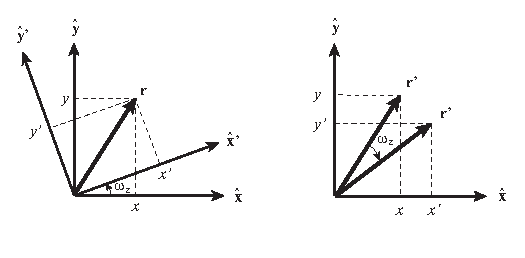
\includegraphics{../figures/appendixC/fig01.eps}
\end{center}
\caption[Active vs passive]{\label{C.fig.passrot}
({\em 左图\/})围绕$\hat{\bf z}$轴旋转了角度$\omega_z$的被动旋转示意图。
观测点的位置矢量${\bf r}=x\hat{\bf x}+y\hat{\bf y}
=x'\hat{\bf x}'+y'\hat{\bf y}'$保持不变。如图所示,当$\omega_z>0$时,坐标轴 $\hat{\bf x}$、$\hat{\bf y}$被逆时针旋转至$\hat{\bf x}'$、$\hat{\bf y}'$。
({\em 右图\/})以等效的主动观点,坐标轴是不变的;而每一点${\bf r}=x\hat{\bf x}+y\hat{\bf y}$被顺时针旋转至新的位置${\bf r}'=x'\hat{\bf x}+y'\hat{\bf y}$。}
\end{figure}
在这个意义上,我们应该将有序序列$\ssR_1,\ssR_2,\ldots$中的每
个被动旋转看作是围绕一系列经过{\em 旋转\/}的轴的旋转$\bomega_1,\bomega_2,\ldots$。
等效的等量且反向的主动旋转系列$-\bomega_1,-\bomega_2,\ldots$是以相同的顺序,但却是围绕{\em 固定\/}的轴(Wolf \citeyear{wolf69})。
由于两个接续有限旋转的顺序是重要的,因此相应的矩阵是不可对易的:$\ssR_2\ssR_1\neq\ssR_1\ssR_2$。
用来“撤销”一个先前的旋转的逆矩阵当然是个例外:$\ssR^{-1}\ssR=\ssR\ssR^{-1}=\ssI$。要“撤销”两个或更多个接续旋转,必须也依照相反的顺序: $(\ssR_2\ssR_1)^{-1}=\ssR_1^{-1}\ssR_2^{-1}$。

我们试图确定旋转$\ssR$或$\bomega$对单位球面$\Omega$上的标量、矢量或更高阶张量场的影响。由于欧氏长度$x^{\prime 2}+y^{\prime 2}+z^{\prime 2}
=x^2+y^2+z^2$在刚性旋转~(\ref{C.Rdef2})下是不变的,我们得到的结果同
样适用于三维空间的场。在下文中,我们将着眼于$\Omega$上的二维场$\psi(\brh)$、
$\bu(\brh)$和$\bT(\brh)$,同时认识到只需放松$x^{\prime 2}+y^{\prime 2}+z^{\prime 2}
=x^2+y^2+z^2=1$这一限制条件,就可以把$\brh$换成$\br$。

一个实数或复数标量场$\psi(\brh)$在每一点$\brh=x\bxh+y\byh+z\bzh
=x'\hat{\bf x}'+y'\hat{\bf y}'+z'\hat{\bf z}'$都有一个确定值。
在原来不带撇的坐标系中,我们以$\psi(x,y,z)$来表示该值。在旋转后的系统中,它由
一个{\em 不同的函数\/}$\psi'(x',y',z')$表示。在每一点$\brh$处,这两个函数具有相同值的条件为:
\eq \label{C.Ddef}
\psi'(x',y',z')=\psi(x,y,z).
\en
我们把~(\ref{C.Ddef})式左右两边的函数当作是用坐标来确定场的数值的规则。
这两个规则是不同的,因为左边的规则在$x'$、$y'$、$z'$的值和右边在$x$、$y$、$z$ 的值必须是相等的。我们试图寻找带撇和不带撇函数之间的关系算子$\sD(\ssR)$或
$\sD(\bomega)$:
\eq \label{C.Ddef2}
\psi'(x,y,z)=\sD(\bomega)\,\psi(x,y,z).
\en
要注意~(\ref{C.Ddef})和~(\ref{C.Ddef2})两式之间的根本区别:
对于后者,自变量$x$、$y$、$z$~(或等价的$x'$、$y'$、$z'$)是哑变量,在两边是一样的。 算子$\sD(\bomega)$可一被认为是对用坐标确定场的数值的{\em 规则做了改变\/}。
如果我们希望得到$\psi'(x',y',z')$,则必须在应用算子$\sD(\bomega)$之前,计算
~(\ref{C.Ddef2})式中原来的函数$\psi$在带撇坐标$x'$、$y'$、$z'$处的值。
通过这一哑变量替换,并与~(\ref{C.Ddef})相比较,我们发现
\eq \label{C.DWolfdef}
\sD(\bomega)\,\psi(x',y',z')=\psi(x,y,z).
\en
(\ref{C.DWolfdef})式也可以用与等量且反向的旋转所对应的{\em 逆旋转算子\/}$\sD^{-1}(\bomega)=\sD(-\bomega)$改写为:
\index{rotation operator!inverse of}%
\index{operator!rotation!inverse of}%
\eq \label{C.DWolfdef2}
\psi(x',y',z')=\sD^{-1}(\bomega)\,\psi(x,y,z).
\en
(\ref{C.DWolfdef2})这一结果提供了对旋转算子的第二个同样有效的解释:逆算子$\sD^{-1}(\bomega)$对$\psi$的作用可以被视为是不改变规则的,但却是做了从$x,y,z$到$x',y',z'$的{\em 坐标改变\/}。在本附录的剩余部分,我们将坚持~(\ref{C.Ddef2})式所表示的第一种解释。

当旋转角度$d\/\bomega$为{\em 无穷小\/}时,
\index{infinitesimal rotation}%
\index{rotation!infinitesimal}%
很容易找到$\psi'$和$\psi$之间的关系;
此时带撇和不带撇的单位矢量之间有如下关系
\eq \label{C.xprxetc}
\bxh'\approx\bxh+d\/\bomega\times\bxh,\qquad
\byh'\approx\byh+d\/\bomega\times\byh,\qquad
\bzh'\approx\bzh+d\/\bomega\times\bzh,
\en
因而旋转矩阵~(\ref{C.Rdef})的形式为
\eq \label{C.Rdef3}
\ssR\approx\left(\begin{array}{ccc}
1 & d\/\omega_z & -d\/\omega_y \\
\vspace{-0.4 ex} & \vspace{-0.4 ex} & \vspace{-0.4 ex} \\
-d\/\omega_z & 1 & d\/\omega_x \\
\vspace{-0.4 ex} & \vspace{-0.4 ex} & \vspace{-0.4 ex} \\
d\/\omega_y & -d\/\omega_x & 1
\end{array}\right).
\en
将~(\ref{C.Rdef2})和~(\ref{C.Rdef3})代入~(\ref{C.Ddef})中,并忽略 $\|d\/\bomega\|$的二阶项,
我们得到$\psi'=\sD(d\bomega)\psi\approx
\psi+(d\/\bomega\times\brh)\cdot\bdel_1\psi$,或者等价的
\eq \label{C.Ddef3}
\sD(d\bomega)\psi\approx(1+i\,d\/\bomega\cdot\bL)\psi,
\en
其中$\bL=-i(\brh\times\bdel_1)=-i[(y\p_z-z\p_y)\bxh
+(z\p_x-x\p_z)\byh+(x\p_y-y\p_x)\bzh]$为角动量算子。
\index{angular-momentum operator}%
\index{operator!angular-momentum}%

有了一阶结果~(\ref{C.Ddef3}),很容易找到控制{\em 有限\/}旋转
\index{finite rotation}%
\index{rotation!finite}%
的算子~(\ref{C.Ddef2})。假设
轴已经过一个初始旋转$\bomega$,因而有$\psi'=\sD(\bomega)\psi$。
进一步的无穷小旋转$d\/\bomega$的影响则为$\psi'=\sD(\bomega+d\bomega)\psi$,其中
\eq \label{C.Dinfdef}
\sD(\bomega+d\/\bomega)\approx
(1+i\,d\/\bomega\cdot\bL)\,\sD(\bomega).
\en
取$d\/\bomega$趋于零的极限,我们看到$\sD(\bomega)$满足一阶常微分方程
\eq \label{C.Ddef4}
d\sD\hspace{-0.3 mm}/\hspace{-0.3 mm}d\bomega
=i\bL\sD.
\en
在$\sD(\bzero)=1$这一边界条件下,方程~(\ref{C.Ddef4})的解为
\eq \label{C.Ddef5}
\sD(\bomega)=\exp(i\bomega\cdot\bL).
\en
角动量算子$\bL$被称为是控制标量场的有限旋转算子~(\ref{C.Ddef5})的{\em 生成算子\/}。
\index{rotation operator!generator of}%
\index{operator!rotation!generator of}%

一个实数或复数矢量场$\bu(\br)$同样可以用两个坐标系中不同的函数$\bu(x,y,z)$和 $\bu'(x',y',z')$表示;
与~(\ref{C.Ddef})式类比,我们必须有
\eq \label{C.uprequ}
\bu'(x',y',z')=\bu(x,y,z).
\en
我们再次引入一个将不带撇场转换到带撇场的旋转算子$\sD(\ssR)$
或$\sD(\bomega)$:
\eq \label{C.vecDdef}
\bu'(x,y,z)=\sD(\bomega)\,\bu(x,y,z).
\en
要得到$\sD(\bomega)$,我们将不带撇场写为$\bu=u_x\bxh+u_y\byh+u_z\bzh$。分量$u_x$、 $u_y$、$u_z$为标量场,在无穷小旋转$d\bomega$下,其变换以算子~(\ref{C.Ddef3})来描述:
\begin{displaymath}
\sD(d\bomega)u_x\approx(1+i\,d\/\bomega\cdot\bL)u_x,\qquad
\sD(d\bomega)u_y\approx(1+i\,d\/\bomega\cdot\bL)u_y,
\end{displaymath}
\eq \label{C.uxyz}
\qquad\qquad\qquad
\sD(d\bomega)u_z\approx(1+i\,d\/\bomega\cdot\bL)u_z.
\en
单位矢量$\bxh$、$\byh$、$\bzh$被同一旋转变换为
\begin{displaymath}
\sD(d\bomega)\bxh\approx\bxh-d\/\bomega\times\bxh,\qquad
\sD(d\bomega)\byh\approx\byh-d\/\bomega\times\byh,
\end{displaymath}
\eq \label{C.Dxxetc}
\qquad\qquad\qquad
\sD(d\bomega)\bzh\approx\bzh-d\/\bomega\times\bzh.
\en
(\ref{C.xprxetc})和~(\ref{C.Dxxetc})之间符号的差异反映了变换的被动性质。如果我们将~(\ref{C.Dxxetc})中的哑笛卡尔轴矢量$\bxh$、$\byh$、$\bzh$换成$\bxh'$、$\byh'$、 $\bzh'$,那么我们可以将变换后的矢量$\sD\bxh'$、$\sD\byh'$、 $\sD\bzh'$视为是原来的矢量在无穷小变换$\sD(d\bomega)$后所“遗留”的“残余”。

我们可以用类似~(\ref{C.uxyz})的形式把~(\ref{C.Dxxetc})式改写为:
\begin{displaymath}
\sD(d\bomega)\bxh\approx(1+i\,d\/\bomega\cdot\bS)\bxh,\qquad
\sD(d\bomega)\byh\approx(1+i\,d\/\bomega\cdot\bS)\byh,
\end{displaymath}
\eq \label{C.vecRdef2}
\qquad\qquad\qquad
\sD(d\bomega)\bzh\approx(1+i\,d\/\bomega\cdot\bS)\bzh.
\en
(\ref{C.vecRdef2})式中的量$\bS=\bxh S_x+\byh S_y+\bzh S_z$是一个矢量算子,
它对单位矢量$\bxh$、$\byh$、$\bzh$的影响可以用显式表示为:
\begin{displaymath}
\bS\bxh=-i(\byh\bzh-\bzh\byh),\qquad
\bS\byh=-i(\bzh\bxh-\bxh\bzh),
\end{displaymath}
\eq \label{C.spinop}
\qquad\qquad\qquad
\bS\bzh=-i(\bxh\byh-\byh\bxh).
\en
很容易证明算子~(\ref{C.spinop})的平方是
\eq
S^2=\bS\cdot\bS=S_x^2+S_y^2+S_z^2=2,
\en
而其自叉乘积则是
\eq \label{C.StimesS}
\bS\times\bS=i\bS.
\en
综合~(\ref{C.uxyz})和~(\ref{C.vecRdef2})的结果,我们得到类似于标量关系~(\ref{C.Ddef3})的矢量变换关系:
\eqa \label{C.boldu} \lefteqn{
\sD(d\bomega)[u_x\bxh+u_y\byh+u_z\bzh]} \nonumber \\
&&\mbox{}\approx \bu+i\,d\/\bomega\cdot[(\bL u_x)\bxh+(\bL u_y)\byh
+(\bL u_z)\bzh \nonumber \\
&&\mbox{}\qquad\qquad
+u_x(\bS\bxh)+u_y(\bS\byh)+u_z(\bS\bzh)].
\ena
在下文中,我们将用下面的简便符号来改写~(\ref{C.boldu})和其它相似的关系式
\eq \label{C.Jdef}
\sD(d\bomega)\bu\approx(1+i\,d\/\bomega\cdot\bJ)\bu\quad\mbox{where}
\quad\bJ=\bL+\bS.
\en
在此处更一般的背景下,矢量$\bL$被称为{\em 轨道\/}角动量算子;
\index{angular-momentum operator!orbital}%
\index{operator!angular-momentum!orbital}%
\index{orbital angular-momentum operator}%
该算子反映了因无穷小旋转$d\/\bomega$而造成的$\psi$或$u_x$、$u_y$、$u_z$对$x$、$y$、 $z$的依赖性的变化。而矢量$\bS$则被称为{\em 自旋\/}角动量算子,
\index{angular-momentum operator!spin}%
\index{operator!angular-momentum!spin}%
\index{spin angular-momentum operator}%
其作用是在不影响分量$u_x$、$u_y$、 $u_z$的同时,根据定义~(\ref{C.spinop})来重整笛卡尔单位矢量$\bxh$、$\byh$、$\bzh$。
将$\bL$和$\bS$合并起来构成一个{\em 总\/}角动量算子
\index{angular-momentum operator!total}%
\index{operator!angular-momentum!total}%
\index{total angular-momentum operator}%
看上去不像是可取的做法,因为$\bL$和$\bS$分别作用于独立的对象;
我们写成$\bJ=\bL+\bS$相加的形式,是基于一个明确的认识,就是将~(\ref{C.Jdef})式只是对较长的~(\ref{C.boldu})式的一个简便的缩写。
在下文中,我们将不再纠缠于区分轨道和自旋角动量,而是直接使用总角动量算子$\bJ$写为
\eqa \label{C.Judef} \lefteqn{
\bJ\bu=(\bJ u_x)\bxh+(\bJ u_y)\byh+(\bJ u_z)\bzh} \nonumber \\
&&\mbox{}\qquad\qquad
+u_x(\bJ\bxh)+u_y(\bJ\byh)+u_z(\bJ\bzh),
\ena
这里我们视$\bJ u_x=\bL u_x$、
$\bJ u_y=\bL u_y$、$\bJ u_z=\bL u_z$以及
$\bJ\bxh=\bS\bxh$、$\bJ\byh=\bS\byh$、$\bJ\bzh=\bS\bzh$为当然的。
$\bJ=\bxh J_x+\byh J_y+\bzh J_z$作用于笛卡尔单位矢量$\bxh$、$\byh$、 $\bzh$的显式结果为
\eq \label{C.Jxunits}
J_x\bxh=\bzero,
\qquad J_x\byh=i\bzh,
\qquad J_x\bzh=-i\byh,
\en
\eq
J_y\bxh=-i\bzh,
\qquad J_y\byh=\bzero,
\qquad J_y\bzh=i\bxh,
\en
\eq \label{C.Jzunits}
J_z\bxh=i\byh,
\qquad J_z\byh=-i\bxh,
\qquad J_z\bzh=\bzero.
\en
(\ref{C.Jxunits})--(\ref{C.Jzunits})式只是将~(\ref{C.spinop})换了一个写法。

利用与从~(\ref{C.Ddef3})到~(\ref{C.Ddef5})一样的推论,我们可以将微分关系$\sD(d\bomega)\approx 1+i\,d\/\bomega\cdot\bJ$积分,而得到与
有限旋转相应的变换关系$\bu'=\sD(\bomega)\bu$:
\eq \label{C.Dtotdef}
\sD(\bomega)=\exp(i\bomega\cdot\bJ).
\en
总角动量算子$\bJ$是矢量场满足的有限旋转算子~(\ref{C.Dtotdef})的生成算子。
\index{rotation operator}%
\index{operator!rotation}%
围绕任一坐标轴旋转了角度$\omega_x$、$\omega_y$、$\omega_z$ 的有限旋转对旋转轴没有影响,
例如:$\exp(i\omega_zJ_z)\bzh=\bzh$。
另一方面,利用指数算子的泰勒级数展开并重新整理展开项,我们发现
$\exp(i\omega_zJ_z)\bxh=\bxh\cos\omega_z-\byh\sin\omega_z$
和$\exp(i\omega_zJ_z)\byh=\bxh\sin\omega_z+\byh\cos\omega_z$。
如图~\ref{C.fig.lastun}所示,这相当于$\bxh$和$\byh$ 被动地顺时针旋转过角度$\omega_z>0$。 
\begin{figure}[!t]
\begin{center}
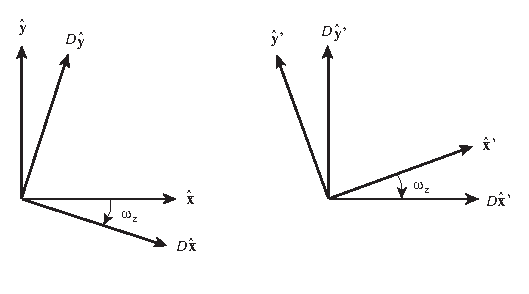
\includegraphics{../figures/appendixC/fig02.eps}
\end{center}
\caption[Last Figure]{\label{C.fig.lastun}
({\em 左图\/})不带撇单位矢量$\hat{\bf x}$$\hat{\bf y}$受算子$\sD=\exp(i\omega_zJ_z)$作用的被动变换。
变换后的矢量$\sD\hat{\bf x}$、
$\sD\hat{\bf y}$被顺时针旋转了角度$\omega_z>0$。
({\em 右图\/})当算子$\sD=\exp(i\omega_zJ_z)$作用于带撇的单位矢量
$\hat{\bf x}'$、$\hat{\bf y}'$时,其结果$\sD\hat{\bf x}'$、
$\sD\hat{\bf y}'$可以被视为是在$\hat{\bf x}'$、$\hat{\bf y}'$的旋转后所“遗留”的矢量$\hat{\bf x}$、$\hat{\bf y}$的"残余"。}
\end{figure}

先是$\bomega_1$再有$\bomega_2$的两个接续有限旋转的结果为:
\eq \label{C.tworots}
\sD(\bomega_2)\sD(\bomega_1)=\exp(i\bomega_2
\cdot\bJ)\exp(i\bomega_1\cdot\bJ),
\en
其中依照惯例,最右边的算子首先作用,然后是最左边的算子。
两个无穷小旋转$d\bomega_1$和$d\bomega_2$的顺序并不重要,因而 $\sD(d\bomega_2)\sD(d\bomega_1)\approx
1+i(d\bomega_2+d\bomega_1)\cdot\bJ\approx
\sD(d\bomega_1)\sD(d\bomega_2)$。
然而,两个有限旋转是不可易的:$\sD(\bomega_2)\sD(\bomega_1)
\neq \sD(\bomega_1)\sD(\bomega_2)$。
旋转算子的逆为:
\eq \label{C.Dinvdef}
\sD^{-1}(\bomega)=\sD(-\bomega)=
\exp(-i\bomega\cdot\bJ).
\en
算子相乘$\sD(\bomega_2)\sD(\bomega_1)$和矩阵相乘 $\ssR_2\ssR_1$是同义的,
且$\sD^{-1}(\bomega)$是与$\ssR^{-1}$相应的算子。

有限旋转算子~(\ref{C.Dtotdef}) 也可以用来描述更高阶张量的变换特性;也就是说,如果$\bT(\br)$是一
个满足$\bT'(x',y',z')=\bT(x,y,z)$的任意阶张量场,则有
\eq \label{C.TprDT}
\bT'(x,y,z)=\sD(\bomega)\,\bT(x,y,z).
\en
对于二阶张量$\bT=T_{xx}\bxh\bxh+T_{xy}
\bxh\byh+\cdots+T_{zz}\bzh\bzh$,(\ref{C.Judef})式可以推广为
\eqa \label{C.JTdef} \lefteqn{
\bJ\bT=(\bJ T_{xx})\bxh\bxh+(\bJ T_{xy})\bxh\byh
+\cdots+(\bJ T_{zz})\bzh\bzh}
\nonumber \\
&&\mbox{}\qquad+T_{xx}(\bJ\bxh)\bxh+T_{xy}(\bJ\bxh)\byh
+\cdots+T_{zz}(\bJ\bzh)\bzh \nonumber \\
&&\mbox{}\qquad\qquad
+T_{xx}\bxh(\bJ\bxh)+T_{xy}\bxh(\bJ\byh)+\cdots+T_{zz}\bzh(\bJ\bzh).
\ena
(\ref{C.JTdef})式可以直接地拓展至任意阶张量;
一般来说,在多并矢的表达式中,$\bJ$ 依序作用于每个分量以及每个单位矢量。作用于两个任意阶的张量$\bT$和$\bP$ 的积的结果是:
\eq
\bJ(\bT\bP)=(\bJ\bT)\bP+\bT(\bJ\bP).
\en
显然,在处理更高阶张量$\bT$时,继续使用传统的符号如$u_x$、$u_y$、$u_z$
和$T_{xx},T_{xy},\ldots,T_{zz}$会相当繁琐。
我们将在~\ref{C.sec.canon}节中使用更合理的角标符号把上述结果在球极坐标中重新表示。

由于轨道和自旋角动量算子作用于不同的对象,它们满足$\bL\times\bS=
-\bS\times\bL$。
将此结果与$\bL\times\bL=i\bL$和$\bS\times\bS=i\bS$两个等式结合, 我们发现总角动量算子的叉乘积为
\eq \label{C.JtimesJ}
\bJ\times\bJ=i\bJ.
\en
我们可以将(\ref{C.JtimesJ})这一结果改写为分量$J_x$、$J_y$、 $J_z$的一组{\em 对易关系式\/}:
\index{angular-momentum operator!commutation relations}%
\index{operator!angular-momentum!commutation relations}%
\index{commutation relations}%
\eq
[J_x,J_y]=iJ_z,
\qquad [J_y,J_z]=iJ_x,
\qquad [J_z,J_x]=iJ_y.
\label{C.Jcom}
\en
总角动量平方算子$J^2=\bJ\cdot\bJ
=J_x^2+J_y^2+J_z^2$与$\bJ$是可对易的,因此与$\bJ$的所有分量也是可对易的:
\eq
[J^2,J_x]=[J^2,J_y]=[J^2,J_z]=0.
\en
此外,$\bJ$与偏导数算子$\p_r$以及任何仅依赖半径$r$ 的标量、矢量或张量函数$f(r)$都是可对易的:
 $[\p_r,\bJ]=\bzero$ and $[f(r),\bJ]=\bzero$。
类比于(\ref{B.ladder})式,我们定义总角动量{\em 阶梯算子\/}$J_{\pm}$为:
\index{ladder operator}%
\index{operator!ladder}%
\eq
J_+=J_x+iJ_y,\qquad J_-=J_x-iJ_y.
\en
这些算子所满足的对易关系为
\eq \label{C.Jpmcom}
[J^2,J_{\pm}]=0,\qquad
[J_z,J_{\pm}]=\pm J_{\pm},\qquad
[J_+,J_-]=2J_z.
\en
用$J_{\pm}$和$J_z$,我们可以将$J^2$表示成以下两种形式的任何一个
\eq \label{C.J2Jpm}
J^2=J_+J_-+J_z^2-J_z=J_-J_++J_z^2+J_z.
\en
(\ref{C.Jcom})--(\ref{C.J2Jpm})中的每一个总角动量关系在
第~B.2节的轨道角动量公式(\ref{B.comm2})--(\ref{eq:L2})中都对应的有一个完全一样的关系式。
\index{angular momentum|)}%

%\section{Spherical Polar Coordinates}
\section{形极坐标}
\index{spherical polar coordinates|(}%
\label{C.sec.canon}

余纬度和经度坐标$\theta$、$\phi$
和$\theta'$、$\phi'$可以用通常的方式与原来的和旋转后的笛卡尔坐标轴$\bxh$、 $\byh$、$\bzh$和$\bxh'$、$\byh'$、$\bzh'$联系起来。
单位球面$\bOmega$上的张量场$\bT(\brh)$的带撇和不带撇表述之间的关系式~(\ref{C.TprDT})可以写为以下形式
\eq \label{C.TprDT2}
\bT'(\theta,\phi)=\sD(\bomega)\,\bT(\theta,\phi).
\en
一个三维场$\bT(\br)$以相同的方式变换,只要将~(\ref{C.TprDT2})中的坐标 $\theta$、$\phi$换成$r$、$\theta$、$\phi$。
其中半径$r$在绕原点$\bzero$的刚性旋转$\bomega$下是不变量。

%\subsection{Transformation of the unit vectors}
\subsection{单位矢量变换}
(\ref{A.needinC})--(\ref{A.need2})将球极单位矢量$\brh$、$\bthetah$、
$\bphih$与笛卡尔单位矢量联系起来。
利用这些关系式以及轨道角动量算子$L_x$、$L_y$、$L_z$ 的球极表达式~(\ref{eq:Lxtp})--(\ref{eq:Lztp}),我们得到
\begin{displaymath}
J_x\brh=\bzero,
\qquad
J_x\bthetah=i(\sin\theta)^{-1}\cos\phi\,\bphih,
\qquad
J_x\bphih=-i(\sin\theta)^{-1}\cos\phi\,\bthetah,
\end{displaymath}
\eq
\en
\begin{displaymath}
J_y\brh=\bzero,
\qquad
J_y\bthetah=i(\sin\theta)^{-1}\sin\phi\,\bphih,
\qquad
J_y\bphih=-i(\sin\theta)^{-1}\sin\phi\,\bthetah,
\end{displaymath}
\eq \label{C.needfin}
\en
\eq \label{C.Jpolvec}
J_z\brh=J_z\bthetah=J_z\bphih=\bzero.
\en
以阶梯算子$J_{\pm}$表示的相应关系式为
\begin{displaymath}
J_{\pm}\brh=\bzero,
\qquad
J_{\pm}\bthetah=i(\sin\theta)^{-1}e^{\pm i\phi}\,\bphih,
\qquad
J_{\pm}\bphih=-i(\sin\theta)^{-1}e^{\pm i\phi}\,\bthetah.
\end{displaymath}
\eq \label{C.Jpolvec2}
\en
角动量平方算子$J^2=J_x^2+J_y^2+J_z^2$的作用 则得到一个标量乘以原来的输入矢量:
\eq \label{C.J2polvec}
J^2\brh=\bzero,\qquad J^2\bthetah=(\sin\theta)^{-2}\bthetah,
\qquad J^2\bphih=(\sin\theta)^{-2}\bphih.
\en
笼统地讲,我们可以将$\brh$、$\bthetah$、$\bphih$视为$J^2$ 的“本征值”为零和$(\sin\theta)^{-2}$的广义本征矢量。在下一节中,我们将引入两个复数单位矢量的三算子组,它们是算子$J_z$、$J_{\pm}$和 $J^2$的共同本征矢量。

%\subsection{Dual canonical bases}
\subsection{对偶正则基}
\label{C.sec.twobases}
\index{canonical basis|(}%
\index{dual canonical basis|(}%
\index{basis!dual canonical|(}%

为加快进度,我们采用便捷的角标符号,其中球极单位矢量表示为
\eq \label{C.italbas}
\beh_1=\brh,\qquad\beh_2=\bthetah,\qquad\beh_3=\bphih.
\en
在本附录中,斜体角标$i,j,k,\ldots$的取值为$\{1,2,3\}$,用于标记矢量和张量相对于这个基的(普通物理)分量。我们定义下、上{\em 正则\/}基矢量 $\beh_-$、$\beh_0$、$\beh_+$和
$\beh^-$、$\beh^0$、$\beh^+$為
\index{canonical basis}%
\eq \label{C.behup}
\beh_-=\textstyle{\frac{1}{\sqrt{2}}}(\bthetah-i\bphih),
\qquad \beh_0=\brh,\qquad
\beh_+=-\textstyle{\frac{1}{\sqrt{2}}}(\bthetah+i\bphih)
\en
和
\eq \label{C.behdown}
\beh^-=\textstyle{\frac{1}{\sqrt{2}}}(\bthetah+i\bphih),
\qquad \beh^0=\brh,\qquad
\beh^+=-\textstyle{\frac{1}{\sqrt{2}}}(\bthetah-i\bphih).
\en
希腊角标$\alpha,\beta,\gamma,\ldots$的取值为$\{-, 0, +\}$或
等价的$\{-1, 0, 1\}$,用来标记上述的两组基。
作为该符号的一个例子,我们指出~(\ref{C.behup}) 和~(\ref{C.behdown})只是互为复数共轭:即$\beh^{\alpha}
=\beh_{\raisebox{0.3 ex}{$\scriptstyle\alpha$}}^*$。此外,每个正则基在下式的意义上都是正交归一的:
\eq \label{C.behortho}
\beh_{\raisebox{0.3 ex}{$\scriptstyle\alpha$}}^*\cdot\beh_{\beta}
=\delta_{\alpha\beta},\qquad
\beh^{\alpha *}\cdot\beh^{\beta}=\delta^{\alpha\beta}.
\en
最后,这两组基{\em 互为对偶\/};即
\index{dual basis}%
\eq \label{C.behdual}
\beh_{\alpha}\cdot\beh^{\beta}=\delta_{\alpha}^{\,\,\,\beta},
\qquad
\beh^{\alpha}\cdot\beh_{\beta}=\delta^{\alpha}_{\,\,\,\beta}.
\en
对于上、下希腊角标做出区分的必要性使我们必须在~(\ref{C.behortho})--(\ref{C.behdual})式中使用所有四个
克罗内克符号$\delta_{\alpha\beta}$、
$\delta^{\alpha\beta}$、$\delta_{\alpha}^{\,\,\,\beta}$
和$\delta^{\alpha}_{\,\,\,\beta}$。

我们可以利用角标符号将定义~(\ref{C.behup})--(\ref{C.behdown})改写为简洁的形式
\eq \label{C.ealphai}
\beh_{\alpha}=(\beh_i\cdot\beh_{\alpha})\,\beh_i,\qquad
\beh^{\alpha}=(\beh_i\cdot\textcolor{red}{\beh^{\alpha}})\,\beh_i.
\en
反之,球极基也可以用正则基来表示
\eq \label{C.eialpha}
\beh_i=(\beh^{\alpha}\cdot\beh_i)\,\beh_{\alpha}
=(\beh_{\alpha}\cdot\beh_i)\,\beh^{\alpha}.
\en
(\ref{C.eialpha})式中的复数矩阵分量$\beh^{\alpha}\cdot\beh_i$和
$\beh_{\alpha}\cdot\beh_i$用显式给定为
\eq \label{C.Cdef}
\left(\begin{array}{ccc}
\beh^-\!\cdot\beh_1 & \beh^0\!\cdot\beh_1 & \beh^+\!\cdot\beh_1 \\
\vspace{-0.4 ex} & \vspace{-0.4 ex} & \vspace{-0.4 ex} \\
\beh^-\!\cdot\beh_2 & \beh^0\!\cdot\beh_2 & \beh^+\!\cdot\beh_2 \\
\vspace{-0.4 ex} & \vspace{-0.4 ex} & \vspace{-0.4 ex} \\
\beh^-\!\cdot\beh_3 & \beh^0\!\cdot\beh_3 & \beh^+\!\cdot\beh_3
\end{array}\right)=
\left(\begin{array}{rrr}
0\hspace{1.5 mm} & 1 & 0\hspace{1.5 mm} \\
\vspace{-0.4 ex} & \vspace{-0.4 ex} & \vspace{-0.4 ex} \\
\textstyle{\frac{1}{\sqrt{2}}} & 0 & -\textstyle{\frac{1}{\sqrt{2}}} \\
\vspace{-0.4 ex} & \vspace{-0.4 ex} & \vspace{-0.4 ex} \\
\textstyle{\frac{i}{\sqrt{2}}} & 0 & \textstyle{\frac{i}{\sqrt{2}}}
\end{array}\right)
\en
和
\eq \label{C.Cdef2}
\left(\begin{array}{ccc}
\beh_-\!\cdot\beh_1 & \beh_0\!\cdot\beh_1 & \beh_+\!\cdot\beh_1 \\
\vspace{-0.4 ex} & \vspace{-0.4 ex} & \vspace{-0.4 ex} \\
\beh_-\!\cdot\beh_2 & \beh_0\!\cdot\beh_2 & \beh_+\!\cdot\beh_2 \\
\vspace{-0.4 ex} & \vspace{-0.4 ex} & \vspace{-0.4 ex} \\
\beh_-\!\cdot\beh_3 & \beh_0\!\cdot\beh_3 & \beh_+\!\cdot\beh_3
\end{array}\right)=
\left(\begin{array}{rrr}
0\hspace{1.5 mm} & 1 & 0\hspace{1.5 mm} \\
\vspace{-0.4 ex} & \vspace{-0.4 ex} & \vspace{-0.4 ex} \\
\textstyle{\frac{1}{\sqrt{2}}} & 0 & -\textstyle{\frac{1}{\sqrt{2}}} \\
\vspace{-0.4 ex} & \vspace{-0.4 ex} & \vspace{-0.4 ex} \\
-\textstyle{\frac{i}{\sqrt{2}}} & 0 & -\textstyle{\frac{i}{\sqrt{2}}}
\end{array}\right).
\en
复数正则基之间的变换为ㄠ正变换,这是因为
\eq \label{C.Cunit}
(\beh_i\cdot\beh_{\alpha})(\beh^{\alpha}\cdot\beh_j)=
(\beh_i\cdot\beh^{\alpha})(\beh_{\alpha}\cdot\beh_j)
=\delta_{ij}.
\en
要注意,(\ref{C.eialpha})和~(\ref{C.Cunit})式中使用了求和惯例。
斜体角标遵循常用的基本规则;而重复希腊角标则必须在上、下不同的位置出现。

两组三矢量正则基$\beh_-$、$\beh_0$、$\beh_+$和
$\beh^-$、$\beh^0$、$\beh^+$实际上就是我们要找的总角动量算子$J_z$、
$J_{\pm}$和$J^2$的共同本征矢量。从~(\ref{C.Jpolvec})--(\ref{C.J2polvec}),我们推导出
\eq
J_z\beh_\alpha=J_z\beh^\alpha=\bzero,
\label{C.Jzsim}
\en
\eq
J_\pm\beh_\alpha=\alpha (\sin\theta)^{-1}e^{\pm i\phi}\,\beh_\alpha,\qquad
J_\pm\beh^\alpha=-\alpha (\sin\theta)^{-1}e^{\pm i\phi}\,\beh^\alpha,
\label{C.Jpmsim}
\en
\eq
J^2\beh_\alpha=\alpha^2(\sin\theta)^{-2}\,\beh_\alpha,\qquad
J^2\beh^\alpha=\alpha^2(\sin\theta)^{-2}\,\beh^\alpha.
\label{C.J2sim}
\en
(\ref{C.Jzsim})--(\ref{C.J2sim})这些结果 在构建广义球谐函数中起到关键性的作用;的确,它们正是引入正则基的动机。
\index{canonical basis|)}%
\index{dual canonical basis|)}%
\index{basis!dual canonical|)}%


%\subsection{Covariant and contravariant components}
\subsection{协变和逆变分量}
\index{component!contravariant|(}%
\index{contravariant component|(}%
\index{component!covariant|(}%
\index{covariant component|(}%

一个$q$阶张量$\bT$可以用其普通球极分量表示成以下形式
\eq
\bT=T_{i_1\cdots i_q}\beh_{i_1}\cdots\beh_{i_q},
\en
其中
\eq \label{C.ordcomdef}
T_{i_1\cdots i_q}=(\beh_{i_1}\cdots\beh_{i_q})\tdot\bT.
\en
同一张量也可用其相对于正则基的{\em 协变\/}和{\em 逆变\/}分量来表示:
\eq
\bT=T_{\alpha_1\cdots\alpha_q}\beh^{\alpha_1}\cdots\beh^{\alpha_q}
=T^{\alpha_1\cdots\alpha_q}\beh_{\alpha_1}\cdots\beh_{\alpha_q},
\en
其中
\eq \label{C.cancomdef}
T_{\alpha_1\cdots\alpha_q}=(\beh_{\alpha_1}
\cdots\beh_{\alpha_q})\tdot\bT,
\en
\eq \label{C.cancomdef2}
T^{\alpha_1\cdots\alpha_q}=(\beh^{\alpha_1}
\cdots\beh^{\alpha_q})\tdot\bT.
\en
分量~(\ref{C.ordcomdef})
和~(\ref{C.cancomdef})--(\ref{C.cancomdef2})之间由幺正变换矩阵~(\ref{C.Cdef})--(\ref{C.Cdef2})相联系:
\eq
T_{\alpha_1\cdots\alpha_q}=(\beh_{\alpha_1}\cdot\beh_{i_1})
\cdots(\beh_{\alpha_q}\cdot\beh_{i_q})\,T_{i_1\cdots i_q},
\en
\eq
T^{\alpha_1\cdots\alpha_q}=(\beh^{\alpha_1}\cdot\beh_{i_1})
\cdots(\beh^{\alpha_q}\cdot\beh_{i_q})\,T_{i_1\cdots i_q}.
\en
还可以定义许多协变-逆变混合的正则分量,如$T_{\alpha_1}^{\,\,\,\,\alpha_2\cdots\alpha_q}=(\beh_{\alpha_1}
\beh^{\alpha_2}\cdots\beh^{\alpha_q})\tdot\bT=
(\beh_{\alpha_1}\cdot\beh_{i_1})(\beh^{\alpha_2}\cdot\beh_{i_2})
\cdots(\beh^{\alpha_q}\cdot\beh_{i_q})\,T_{i_1\cdots i_q}$。

一个矢量可以写成$\bu=u_{\alpha}\beh^{\alpha}=
u^{\alpha}\beh_{\alpha}$,其中$u_{\alpha}=\beh_{\alpha}\cdot\bu$
和$u^{\alpha}=\beh^{\alpha}\cdot\bu$。一个二阶张量有四种
正则形式:
\eq
\bT=T_{\alpha\beta}\beh^{\alpha}\beh^{\beta}=
T^{\alpha\beta}\beh_{\alpha}\beh_{\beta}=
T_{\alpha}^{\,\,\,\beta}\beh^{\alpha}\beh_{\beta}=
T^{\alpha}_{\,\,\,\beta}\beh_{\alpha}\beh^{\beta},
\en
其中
\eq \label{C.ten2com}
T_{\alpha\beta}=\beh_{\alpha}\cdot\bT\cdot\beh_{\beta},\qquad
T^{\alpha\beta}=\beh^{\alpha}\cdot\bT\cdot\beh^{\beta},
\en
\eq \label{C.ten2com2}
T_{\alpha}^{\,\,\,\beta}=\beh_{\alpha}\cdot\bT\cdot\beh^{\beta},\qquad
T^{\alpha}_{\,\,\,\beta}=\beh^{\alpha}\cdot\bT\cdot\beh_{\beta}.
\en
一个对称张量$\bT=\bT^{\rm T}$的分量~(\ref{C.ten2com})--(\ref{C.ten2com2})
满足对称关系$T_{\alpha\beta}=T_{\beta\alpha}$、 $T^{\alpha\beta}=T^{\beta\alpha}$
和$T_{\alpha}^{\,\,\,\beta}=T^{\beta}_{\,\,\,\alpha}$、
$T^{\alpha}_{\,\,\,\beta}=T_{\beta}^{\,\,\,\alpha}$。

单位张量$\bI$的协变和逆变分量为:
\eq
g_{\alpha\beta}=\beh_\alpha\cdot\beh_\beta,\qquad
g^{\alpha\beta}=\beh^\alpha\cdot\beh^\beta,
\en
或者等价于
\eqa \label{C.metric} \lefteqn{
\left(\begin{array}{lll}
g_{--} & g_{-0} & g_{-+} \\
\vspace{-0.4 ex} & \vspace{-0.4 ex} & \vspace{-0.4 ex} \\
g_{0-} & g_{00} & g_{0+} \\
\vspace{-0.4 ex} & \vspace{-0.4 ex} & \vspace{-0.4 ex} \\
g_{+-} & g_{+0} & g_{++}
\end{array}\right)
=\left(\begin{array}{lll}
g^{--} & g^{-0} & g^{-+} \\
\vspace{-0.4 ex} & \vspace{-0.4 ex} & \vspace{-0.4 ex} \\
g^{0-} & g^{00} & g^{0+} \\
\vspace{-0.4 ex} & \vspace{-0.4 ex} & \vspace{-0.4 ex} \\
g^{+-} & g^{+0} & g^{++}
\end{array}\right)} \nonumber \\
&&\hspace{2.77cm}\mbox{}=\left(\begin{array}{rrr}
0 & 0 & -1 \\
\vspace{-0.4 ex} & \vspace{-0.4 ex} & \vspace{-0.4 ex} \\
0 & 1 & 0 \\
\vspace{-0.4 ex} & \vspace{-0.4 ex} & \vspace{-0.4 ex} \\
-1 & 0 & 0
\end{array}\right).
\ena
根据对偶关系~(\ref{C.behdual}),混合分量$g_{\alpha}^{\,\,\,\beta}  \vspace{-0.4 mm}
=\beh_{\alpha}\cdot\beh^{\beta}$和
$g^{\alpha}_{\,\,\,\beta}
=\beh^{\alpha}\cdot\beh_{\beta}$只是克罗内克符号 $\delta_{\alpha}^{\,\,\,\beta}$
和$\delta^{\alpha}_{\,\,\,\beta}$。
我们可以将$g_{\alpha\beta}$和$g^{\beta\alpha}$这两个量视为{\em 度量张量\/}的协变和逆变分量,
\index{metric tensor}%
\index{tensor!metric}%
用惯常的做法,它们可以将希腊角标上升和下降。因此对一个矢量$\bu$有
\eq
u_{\alpha}=g_{\alpha\beta}u^{\beta},\qquad
u^{\alpha}=g^{\alpha\beta}u_{\beta},
\en
而对一个二阶张量$\bT$则有:
\eq
T_{\alpha\beta}=g_{\alpha\gamma}T^{\gamma}_{\,\,\,\beta}
=g_{\alpha\gamma}g_{\beta\eta}T^{\gamma\eta},\qquad
T^{\alpha\beta}=g^{\alpha\gamma}T_{\gamma}^{\,\,\,\beta}
=g^{\alpha\gamma}g^{\beta\eta}T_{\gamma\eta}
\en
我们可以将$\bI$用其分量表示任何一种等价形式:
$\bI=g_{\alpha\beta}\beh^{\alpha}\beh^{\beta}
=g^{\alpha\beta}\beh_{\alpha}\beh_{\beta}
=\beh^{\alpha}\beh_{\alpha}=\beh_{\alpha}\beh^{\alpha}$

三阶交替张量$\bLambda$的协变和逆变分量为
\eq
\ep_{\alpha\beta\gamma}=\beh_{\alpha}\cdot
(\beh_{\beta}\times\beh_{\gamma}),\qquad
\ep^{\alpha\beta\gamma}=\beh^{\alpha}\cdot
(\beh^{\beta}\times\beh^{\gamma}).
\en
$\ep_{\alpha\beta\gamma}$和
$\ep^{\alpha\beta\gamma}$与Levi-Civit\`{a}交替符号 $\ep_{ijk}$拥有相同的排列性质;事实上
\eq \label{C.eps1}
\ep_{\alpha\beta\gamma}=\left\{\begin{array}{rl}
i & \mbox{当 $\alpha,\beta,\gamma$ 为 $-,0,+$ 的偶数排列时} \\
-i & \mbox{当 $\alpha,\beta,\gamma$ 为 $-,0,+$ 的奇数排列时} \\
0 & \mbox{其余情形}
\end{array}\right.
\en
和
\eq \label{C.eps2}
\ep^{\alpha\beta\gamma}
=\left\{\begin{array}{rl}
-i & \mbox{当 $\alpha,\beta,\gamma$ 为 $-,0,+$ 的偶数排列时} \\
i & \mbox{当 $\alpha,\beta,\gamma$ 为 $-,0,+$ 的奇数排列时} \\
0 & \mbox{其余情形.}
\end{array}\right.
\en
交替张量可以写为
$\bLambda=\eps_{\alpha\beta\gamma}\beh^{\alpha}\beh^{\beta}\beh^{\gamma}
=\eps^{\alpha\beta\gamma}\beh_{\alpha}\beh_{\beta}\beh_{\gamma}$.
\index{component!contravariant|)}%
\index{contravariant component|)}%
\index{component!covariant|)}%
\index{covariant component|)}%

%\subsection{Dot and cross products}
\subsection{点积与叉乘积}
\index{dot product|(}%
\index{cross product|(}%

两个矢量的点积$\bu\cdot\bv=u_iv_i$ 的正则表达式可以写成下面四个等价形式中的任何一个
\eq
u_{\alpha}v^{\alpha}=u^{\alpha}v_{\alpha}=
g_{\alpha\beta}u^{\alpha}v^{\beta}
=g^{\alpha\beta}u_{\alpha}v_{\beta}.
\en
同样地,两个二阶张量的双点积$\bT\!:\!\bP=T_{ij}P_{ij}$可以写为
\eq
T_{\alpha\beta}P^{\alpha\beta}=
T^{\alpha\beta}P_{\alpha\beta}=g_{\alpha\gamma}
g_{\beta\eta}T^{\alpha\beta}P^{\gamma\eta}=
g^{\alpha\gamma}g^{\beta\eta}T_{\alpha\beta}P_{\gamma\eta},
\en
以及一些涉及混合分量$T_{\alpha}^{\,\,\,\beta}$、
$T^{\alpha}_{\,\,\,\beta}$和$P_{\alpha}^{\,\,\,\beta}$、
$P^{\alpha}_{\,\,\,\beta}$的间接表达式。
两个矢量的叉乘积$\bw=\bu\times\bv$
可以用纯协变和逆变的交替符号~(\ref{C.eps1})--(\ref{C.eps2})表示为
\eq
w_{\alpha}=\ep_{\alpha\beta\gamma}u^{\beta}v^{\gamma},\qquad
w^{\alpha}=\ep^{\alpha\beta\gamma}u_{\beta}v_{\gamma}.
\en
对此更是有一大批涉及度量张量的协变和逆变分量以及交替张量的混合分量的等价的间接关系式存在。

为简单起见,我们在之后所有涉及到物理矢量和张量变量$\bu$和 $\bT$的计算中,都将用它们的{\em 逆变\/}分量$u^{\alpha}$和 $T^{\alpha_1\cdots\alpha_q}$来进行。
\index{component!contravariant}%
\index{contravariant component}%
\index{component!covariant}%
\index{covariant component}%
唯一用到的协变分量是单位张量$g_{\alpha\beta}$和交替张量 $\ep_{\alpha\beta\gamma}$的;混合分量将完全避免使用。
两个矢量的点积$\bu\cdot\bv=g_{\alpha\beta}u^{\alpha}v^{\beta}$ 
和两个张量的双点积$\bT\!:\!\bP=g_{\alpha\gamma}
g_{\beta\eta}T^{\alpha\beta}P^{\gamma\eta}$的逆变分量显式表达式为
\eq \label{C.udotv}
\bu\cdot\bv=-u^-v^++u^0v^0-u^+v^-,
\en
\eqa \label{C.TddotP} \lefteqn{
\bT\!:\!\bP=T^{--}P^{++}-T^{-0}P^{+0}+T^{-+}P^{+-}} \nonumber \\
&&\mbox{}\qquad-T^{0-}P^{0+}+T^{00}P^{00}-T^{0+}P^{0-} \nonumber \\
&&\mbox{}\qquad\qquad+T^{+-}P^{-+}-T^{+0}P^{-0}+T^{++}P^{--}.
\ena
矢量叉乘积的逆变分量$w^{\alpha}=g^{\alpha\eta}
\ep_{\eta\beta\gamma}u^{\beta}v^{\gamma}$为$w^-=i(u^0v^--u^-v^0)$、 $w^0=i(u^+v^--u^-v^+)$
和$w^+=i(u^+v^0-u^0v^+)$。

两个更高阶张量的缩并可以用它们的逆变分量写为
\eq \label{C.TtdotP}
\bT\tdot\bP=g_{\alpha_1\beta_1}\cdots g_{\alpha_q\beta_q}
T^{\alpha_1\cdots\alpha_q}P^{\beta_1\cdots\beta_q}.
\en
利用正交归一关系~(\ref{C.behortho}),涉及到复数共轭的缩并比~(\ref{C.TtdotP})更为简单:
\eq \label{C.TtdotP2}
\bT^*\tdot\bP=\delta_{\alpha_1\beta_1}\cdots\delta_{\alpha_q\beta_q}
T^{\alpha_1\cdots\alpha_q\textcolor{red}{*}}P^{\beta_1\cdots\beta_q}.
\en
(\ref{C.TtdotP2})式右边似乎应该写为更简洁的形式$T^{\alpha_1\cdots\alpha_q}P^{\alpha_1\cdots\alpha_q}$;然而这样做会违背我们的重复希腊角标必须出现在上、下不同位置的规定。
\index{dot product|)}%
\index{cross product|)}%

%\subsection{Hermiticity of J}
\subsection{算子J的厄米特性质}
\index{angular-momentum operator!Hermiticity of|(}%
\index{operator!angular-momentum!Hermiticity of|(}%

单位球面$\Omega$上的两个复数张量场$\bT$和$\bP$的内积~(\ref{C.inprod}) 的分量表达式为
\eq \label{C.inprod2}
\langle\bT,\bP\rangle=\int_{\Omega}\delta_{\alpha_1\beta_1}
\cdots\delta_{\alpha_q\beta_q}
T^{\alpha_1\cdots\alpha_q *}P^{\beta_1\cdots\beta_q}\,d\/\Omega.
\en
有了~(\ref{C.inprod2}),我们终于做好了准备,能够来建立总角动量算子是自伴随或厄米特的这一重要结果:
\eq
\bJ^{\dagger}=\bJ.
\en

如同附录B中轨道角动量的例子,对球极分量$J_z$的讨论是最简单的。
由于该算子无论对正则基矢量还是度量张量都没有影响,
因此如同在(\ref{B.Hermproof})式中一样对$\phi$进行部分积分就足以证明
$\langle\bT,J_z\bP\rangle
=\langle J_z\bT,\bP\rangle$。
直接证明$\langle\bT,J_x\bP\rangle
=\langle J_x\bT,\bP\rangle$和
$\langle\bT,J_y\bP\rangle
=\langle J_y\bT,\bP\rangle$是比较复杂的;然而,
我们还是可以依赖一个论据,就是由于笛卡尔坐标轴$\bxh$、$\byh$、$\bzh$ 可以任意选择,因此$J_z^{\dagger}=J_z$意味着$J_x^{\dagger}=J_x$和 $J_y^{\dagger}=J_y$。
角动量平方算子也是厄米特的,而两个阶梯算子则互为彼此的伴随算子:$(J^2)^{\dagger}=J^2$和$(J_{\pm})^{\dagger}=J_{\mp}$。
$\sD(\bomega)=\exp(i\bomega\cdot\bJ)$的伴随是
$\sD^{\dagger}(\bomega)=\exp(-i\bomega\cdot\bJ)$。由于其伴随算子和逆算子是相同的,即
\eq \label{C.Dadjdef}
\sD^{\dagger}(\bomega)=\sD^{-1}(\bomega),
\en
因而有限旋转算子为{\em ㄠ正\/}的。
\index{unitary operator}%
\index{operator!unitary}%
\index{angular-momentum operator!Hermiticity of|)}%
\index{operator!angular-momentum!Hermiticity of|)}%
\index{spherical polar coordinates|)}%


%\section{Construction of a Basis}
\section{基的构建}
\index{generalized spherical harmonics!basis construction|(}%
\index{spherical harmonics!generalized!basis construction|(}%

遵循与第~\ref{sec:conbas}节中相同的步骤,我们建构一个作为可对易的厄密特算子$J^2$和$J_z$的共同本征函数的广义表面球谐函数的正交归一基。我们以 $\bY_{lm}^N(\theta,\phi)$ 来表示这些局限于单位球表面的球谐函数,并且类比于~(\ref{B.simult})而规范
\eq \label{C.Jeig}
J^2\bY_{lm}^N=l(l+1)\bY_{lm}^N,\qquad
J_z\bY_{lm}^N=m\bY_{lm}^N.
\en
假设$\bY_{lm}^N$为$q$阶张量,我们将其用正则基矢量展开为
\eq \label{C.YlmNdef}
\bY_{lm}^N=Y_{lm}^N\textcolor{red}{\beh_{\alpha_1}\cdots\beh_{\alpha_q}}.
\en
我们称$\bY_{lm}^N$为{\em 张量\/}球谐函数,
\index{tensor harmonic}%
\index{scalar harmonic}%
而称$Y_{lm}^N$为相应的{\em 标量\/}球谐函数。
与前面一样,该张量和标量的下角标是球谐函数的{\em 次数\/}$l$和{\em 级数\/}$m$;
\index{degree}%
\index{spherical harmonics!generalized!degree of}%
\index{generalized spherical harmonics!degree of}%
\index{order}%
\index{spherical harmonics!generalized!order of}%
\index{generalized spherical harmonics!order of}%
我们下面会看到,上角标$N$依赖于张量$\bY_{lm}^N$的阶数$q$。
本征值方程~(\ref{C.Jeig})中的第二个方程意味着每个标量球谐函数都必须具有以下形式
\eq
Y_{lm}^N(\theta,\phi)=X_{lm}^N(\theta)\exp(im\phi).
\en
上式表明级数$m$必须为整数,以确保$Y_{lm}^N$在单位球上是单值的。
每个广义表面球谐函数都由关系 $\bY_{lm}^N(\br)=r^l\bY_{lm}^N(\theta,\phi)$生成
一个相应的立体球谐函数;然而,这些三维函数在理论中没有任何重要作用。

类比于~(\ref{B.LADDER})--(\ref{eq:Lladder}),
我们可利用对易关系~(\ref{C.Jpmcom})证明张量$J_\pm\bY_{lm}^N$ 
为$J^2$和$J_z$的本征值分别为$l(l+1)$和$m\pm 1$的本征函数:
\eq \label{C.LADDER}
J^2(J_\pm\bY_{lm}^N)=J_\pm(J^2\bY_{lm}^N)=l(l+1)(J_\pm\bY_{lm}^N),
\en
\eq
J_z(J_\pm\bY_{lm}^N)=(J_\pm J_z\pm J_\pm)\bY_{lm}^N
=(m\pm 1)(J_\pm\bY_{lm}^N).
\label{eq:Jladder}
\en
{\em 升阶\/}算子$J_+$
\index{ladder operator!ascending}%
\index{operator!ladder!ascending}%
将$\bY_{lm}^N$变换为一个常数乘以$\bY_{l\,m+1}^N$,而{\em 降阶\/}算子
\index{ladder operator!descending}%
\index{operator!ladder!descending}%
则将其变换为常数乘以$\bY_{l\,m-1}^N$:
\eq
J_\pm\bY_{lm}^N=c_\pm\bY_{l\,m\pm1}^N.
\label{eq:Jcpm}
\en
与推导~(\ref{B.Ylmpm})所用的论据一样,张量$J_{\pm}\bY_{lm}^N$和 $\bY_{lm}^N$的平方泛数之间有关系:
\eq \label{C.Ylmpm}
\|\hspace{-0.3 mm}|J_\pm\bY_{lm}^N\|\hspace{-0.3 mm}|^2
=(l\mp m)(l\pm m+1)\,\|\hspace{-0.3 mm}|\bY_{lm}^N\|\hspace{-0.3 mm}|^2.
\en
将阶梯算子$J_{\pm}$ \vspace{-0.3 mm}
重复作用于$\bY_{l\,\mp l}^N$,最终得到$J_{\pm}\bY_{l\,\pm l}^N=\bzero$这一结果。
阶梯算子在$2l+1$次作用后的终止意味着其
次数$l$必须是正的半整数或整数。在量子力学中,有必要用半整数的量子数来描述具有自旋的质点和质点系统的角动量;
然而在我们这里,由于$m$是整数,因此$l$也必须为整数。
因此,对每一个非负数的次数$l$,都有$2l+1$个整数级数$-l\leq m\leq l$。

由于$J^2$和$J_z$这两个算子的厄米特性质,具有不同次数$l\neq l'$、级数$m\neq m'$和上角标$N\neq N'$的两个广义球谐函数$\bY_{lm}^N$
和$\bY_{l'm'}^{N'}$是正交的。通过以下条件
\eq \label{C.YlmNnorm}
\langle\bY_{lm}^N,\bY_{l'm'}^{N'}\rangle=
\int_{\Omega}\bY_{lm}^{N*}\tdot\bY_{l'm'}^{N'}\,
d\/\Omega=\delta_{ll'}\delta_{mm'}\delta_{N\!N'},
\en
我们得到{\em 正交归一\/}的基。
\index{generalized spherical harmonics!orthonormality}%
\index{spherical harmonics!generalized!orthonormality}%
结合方程~(\ref{eq:Jcpm})和~(\ref{C.YlmNnorm}),我们发现常数$c_{\pm}$ 满足$|c_\pm|^2=(l\mp m)(l\pm m+1)$。

通过将阶梯终止关系$J_{\pm}\bY_{l\,\pm l}^N=\bzero$做显式展开
\eqa \label{C.limharm2} \lefteqn{
J_{\pm}[X_{l\,\pm l}^N(\theta)\exp(\textcolor{red}{\pm il}\phi)
\beh_{\alpha_1}\cdots\beh_{\alpha_q}]} \nonumber \\
&&\mbox{}=[J_{\pm}X_{l\,\pm l}^N(\theta)\exp(\textcolor{red}{\pm il}\phi)]
\beh_{\alpha_1}\cdots\beh_{\alpha_q} \nonumber \\
&&\mbox{}\qquad\qquad+X_{l\,\pm l}^N(\theta)\exp(\textcolor{red}{\pm il}\phi)
(J_{\pm}\beh_{\alpha_1})\cdots\beh_{\alpha_q} \nonumber \\
&&\qquad\qquad\qquad\qquad\qquad\vdots \nonumber \\
&&\mbox{}\qquad\qquad+X_{l\,\pm l}^N(\theta)\exp(\textcolor{red}{\pm il}\phi)
\beh_{\alpha_1}\cdots(J_{\pm}\beh_{\alpha_q})
=\bzero,
\ena
可以得到最高与最低级数的球谐函数$\bY_{l\,\pm l}^N$。
利用~(\ref{B.sphlad})和~(\ref{C.Jpmsim})中的结果,我们得到一个类似于~(\ref{B.Xlleqn})的随余纬度变化的变量函数$X_{l\,\pm l}^N(\theta)$所满足的常微分方程:
\eq \label{eq:X}
\left[\frac{d}{d\theta}-l\cot\theta
\pm N(\sin\theta)^{-1}\right]X_{l\,\pm l}^N=0,
\en
这里我们终于第一次得到了上角标的大小
\eq
N=\alpha_1+\cdots+\alpha_q.
\en
方程~(\ref{eq:X})的解为$X_{l\,\pm l}^N=A_{\pm}
(\sin\half\theta)^{l\textcolor{red}{\mp}N}(\cos\half\theta)^{l\textcolor{red}{\pm}N}$。
为确保常规性,整数$N$必须在$-l\leq N\leq l$的范围内。
模量$|A_{\pm}|$可以通过$\|\hspace{-0.3 mm}|\bY_{l\,\pm l}^N\|\hspace{-0.3 mm}|=1$这一条件来确定。
同在标量的情形一样,常数$c_{\pm}$和$A_{\pm}$的符号仍可任意选择。

选择${\rm sgn}\,A_-=1$和${\rm sgn}\,c_+=1$,并从最低级数的 基元素沿阶梯上升,我们得到广义球谐函数
\eqa \label{C.defi1}
\lefteqn{\bY_{l\,-l}^N=
\left(\frac{2l+1}{4\pi}\right)^{1/2}\left[\frac{(2l)!}
{(l+N)!(l-N)!}\right]^{1/2}} \nonumber \\
&&\mbox{}\times(\sin\half\theta)^{l+N}(\cos\half\theta)^{l-N}
e^{-il\phi}\,\beh_{\alpha_1}\cdots\beh_{\alpha_q}
\ena
和
\eq \label{C.defi2}
\bY_{lm}^N=\left[\frac{(l-m)!}{(l+m)!}\right]^{1/2}
\left[\frac{1}{(2l)!}\right]^{1/2}(J_+)^{l+m}\,\bY_{l-l}^N.
\en
选择${\rm sgn}\,A_+=(-1)^{l+N}$和${\rm sgn}\,c_-=1$,并从最高级数的元素沿阶梯下降,
则可得到另一个等价的表达式:
\eqa \label{C.defi3}
\lefteqn{\bY_{ll}^N=
(-1)^{l+N}\left(\frac{2l+1}{4\pi}\right)^{1/2}\left[\frac{(2l)!}
{(l+N)!(l-N)!}\right]^{1/2}} \nonumber \\
&&\mbox{}\times(\sin\half\theta)^{l-N}(\cos\half\theta)^{l+N}
e^{il\phi}\,\beh_{\alpha_1}\cdots\beh_{\alpha_q}
\ena
和
\eq \label{C.defi4}
\bY_{lm}^N=\left[\frac{(l+m)!}{(l-m)!}\right]^{1/2}
\left[\frac{1}{(2l)!}\right]^{1/2}(J_-)^{l-m}\,\bY_{ll}^N.
\en
(\ref{C.defi1})--(\ref{C.defi2})
和~(\ref{C.defi3})--(\ref{C.defi4})中的定义对所有取值范围为
\eq \label{C.range}
0\leq l\leq\infty,\qquad -l\leq m\leq l,\qquad -l\leq N\leq l,
\en
的整数次数$l$、级数$m$和上角标$N=\alpha_1+\cdots +\alpha_q$成立。
用这一方式定义的广义球谐函数$\bY_{lm}^N$满足本征值关系~(\ref{C.Jeig})、
正交归一关系~(\ref{C.YlmNnorm})以及阶梯算子关系
\eq \label{C.Jladfin}
J_{\pm}\bY_{lm}^N=\sqrt{(l\mp m)(l\pm m+1)}\,
\bY_{l\,m\pm 1}^N.
\en
在~(\ref{C.range})的范围之外,即$|m|>l$以及$|N|>l$,可以简便地定义
$\bY_{lm}^N=\bzero$。这便使得~(\ref{C.Jladfin})式
对于所有的$m$值都成立,如同其标量的对应关系式~(\ref{B.ladfin})。
将~(\ref{C.defi1})--(\ref{C.defi4})式与普通球谐函数相应的定义~(\ref{eq:first})--(\ref{eq:def2})相比较,
我们得到$Y_{lm}^0=Y_{lm}$;这正是我们做上述符号选择的动机。

通过归纳,可以证明(\ref{B.Jpmugly})式的推广形式为:
\eqa
\lefteqn{(J_{\pm})^{l\pm m}\left[ (\sin\half\theta)^{l\pm N}
(\cos\half\theta)^{l\mp N}e^{\mp il\phi}\,
\beh_{\alpha_1}\cdots\beh_{\alpha_q}\right]} \nonumber \\
&&\mbox{}=\,\,\Biggr\{2^{l\pm m}(\sin\half\theta)^{\pm m\mp N}
(\cos\half\theta)^{\pm m\pm N}\Biggl. \nonumber \\
&&\mbox{}\times\left.\left(\pm \frac{1}{\sin\theta}\frac{d}
{d\theta}\right)^{l\pm m}
\left[(\sin\half\theta)^{2l\pm 2N}
(\cos\half\theta)^{2l\mp 2N}\right]\right\} \nonumber \\
&&\mbox{}\times e^{im\phi}\,\beh_{\alpha_1}\cdots\beh_{\alpha_q}.
\label{C.Jpmugly}
\ena
将~(\ref{C.Jpmugly})这一结果用于~(\ref{C.defi1})--(\ref{C.defi4}),我们得到显式表达式
\eqa
\lefteqn{\bY_{lm}^N=\left(\frac{2l+1}{4\pi}\right)^{1/2}
\left[\frac{1}{(l+N)!(l-N)!}\right]^{1/2}
\left[\frac{(l-m)!}{(l+m)!}\right]^{1/2}} \nonumber \\
&&\mbox{}\times\Biggl\{2^{l+m}(\sin\half\theta)^{m-N}
(\cos\half\theta)^{m+N}\biggr. \nonumber \\
&&\mbox{}\times\left.\left(\frac{1}{\sin\theta}
\frac{d}{d\theta}\right)^{l+m}
\left[(\sin\half\theta)^{2l+2N}(\cos\half\theta)^{2l-2N}\right]\right\}
\nonumber \\
&&\mbox{}\times e^{im\phi}\,\beh_{\alpha_1}\cdots\beh_{\alpha_q} \nonumber \\
&&\mbox{}=(-1)^{l-N}\left(\frac{2l+1}{4\pi}\right)^{1/2}
\left[\frac{1}{(l+N)!(l-N)!}\right]^{1/2}
\left[\frac{(l+m)!}{(l-m)!}\right]^{1/2} \nonumber \\
&&\mbox{}\times\Biggl\{2^{l-m}(\sin\half\theta)^{-m+N}
(\cos\half\theta)^{-m-N}\biggr. \nonumber \\
&&\mbox{}\times\left.\left(-\frac{1}{\sin\theta}
\frac{d}{d\theta}\right)^{l-m}
\left[(\sin\half\theta)^{2l-2N}(\cos\half\theta)^{2l+2N}\right]\right\}
\nonumber \\
&&\mbox{}\times e^{im\phi}\,\beh_{\alpha_1}\cdots\beh_{\alpha_q}.
\ena
对比上式中的两个表达式,我们推出
\eq \label{C.YlmNstar}
\bY_{l\,-m}^{-N}=(-1)^m\bY_{lm}^{N*},
\en
上式为对称关系~(\ref{B.Ylmstar})的推广。
在得到~(\ref{C.YlmNstar})的过程中,
我们利用了$\beh_{-\alpha_1}\cdots\beh_{-\alpha_q}=
(-1)^N(\beh_{\alpha_1}\cdots\beh_{\alpha_q})^*$这一事实。

在这一节的最后,我们指出上述符号的含糊性。
符号$Y_{lm}^N$表示一个唯一的标量广义球谐函数;然而, $\bY_{lm}^N$实际上却是一组无穷多的阶数$q>|N|$的张量的缩写:
\begin{displaymath}
\bY_{lm}^0=\{Y_{lm}^0,\,Y_{lm}^0\beh_0,\,Y_{lm}^0\beh_0\beh_0,\,
Y_{lm}^0\beh_-\beh_+,\,Y_{lm}^0\beh_+\beh_-,\ldots\},
\end{displaymath}
\begin{displaymath}
\bY_{lm}^{\pm 1}=\{Y_{lm}^{\pm 1}\beh_{\pm},\,
Y_{lm}^{\pm 1}\beh_0\beh_{\pm},\,
Y_{lm}^{\pm 1}\beh_{\pm}\beh_0,\ldots\},
\end{displaymath}
\begin{displaymath}
\bY_{lm}^{\pm 2}=\{Y_{lm}^{\pm 2}\beh_{\pm}\beh_{\pm},\ldots\},
\end{displaymath}
\eq
\qquad\qquad\qquad\qquad
\vdots .
\en
每一个具有$\alpha_1+\cdots+\alpha_q=N$的有序多并矢 $\beh_{\alpha_1}\cdots\beh_{\alpha_q}$都对应于
相同的广义标量球谐函数$Y_{lm}^N$。
标量球谐函数满足:
\eq \label{C.YlmNminus}
Y_{l\,-m}^{-N}=(-1)^{m+N}Y_{lm}^{N*}.
\en
由于相应的多并矢的正交性,
两个具有不同上角标$N\neq N'$的广义球谐函数$\bY_{lm}^N$和 $\bY_{l'm'}^{N'}$是正交的。
另一方面,当$N=N'$时,(\ref{C.YlmNnorm})式意味着
\eq \label{C.YlmNnorm2}
\int_{\Omega}Y_{lm}^{N*}\,Y_{l'm'}^N\,
d\/\Omega=\delta_{ll'}\delta_{mm'}.
\en
涉及$N\neq N'$的两个标量球谐函数乘积$Y_{lm}^{N*}\,Y_{l'm'}^{N'}$的面积分
在实际中从未出现过。
\index{generalized spherical harmonics!basis construction|)}%
\index{spherical harmonics!generalized!basis construction|)}%

%\section{Generalized Legendre Functions}
\section{广义勒让德函数}
\index{generalized Legendre function|(}%
\index{Legendre function!generalized|(}%

将表达式$\bY_{lm}^N(\theta,\phi)=
X_{lm}^N(\theta)e^{im\phi}\beh_{\alpha_1}\cdots\beh_{\alpha_q}$代入本征值问题$J^2\bY_{lm}^N=l(l+1)\bY_{lm}^N$,我们发现余纬度的标量函数$X_{lm}^N$满足常微分方程
\eqa \label{C.genLeg} \lefteqn{
(1-\mu^2)\frac{d^2X}{d\mu^2}-2\mu\frac{dX}{d\mu}} \nonumber \\
&&\mbox{}+\left[l(l+1)-\frac{m^2-2mN\mu+N^2}
{1-\mu^2}\right]X=0,
\ena
其中$\mu=\cos\theta$。如预期的,所谓的{\em 广义勒让德方程\/}~(\ref{C.genLeg})在 $N=0$时简化为普通勒让德方程~(\ref{eq:Legeqn2})。
\index{Legendre equation!generalized}%
\index{generalized Legendre equation}%
遵循\textcite{phinney&burridge73},
我们定义次数$l$、级数$-l\leq m\leq l$以及上角标$-l\leq N\leq l$ 的{\em 广义勒让德函数\/}为
\eqa
\lefteqn{P_{lm}^N(\mu)=\frac{1}{2^l}
\left[\frac{1}{(l+N)!(l-N)!}\right]^{1/2}
\left[\frac{(l+m)!}{(l-m)!}\right]^{1/2}} \nonumber \\
&&\mbox{}\times(1-\mu)^{-\half(m-N)}(1+\mu)^{-\half(m+N)} \nonumber \\
&&\mbox{}\times\left(\frac{d}{d\mu}\right)^{l-m}\left[(\mu-1)^{l-N}
(\mu+1)^{l+N}\right]. \label{eq:polyno}
\ena
方程~(\ref{C.genLeg})在$-1\leq\mu\leq 1$范围内的这些正规解
在$N=0$时{\em 并不简化为\/}连带勒让德函数$P_{lm}(\mu)$;事实上有
\eq
%---label added by H.-Y. Yang----
\label{C.Plm0-Plm}
%-----------------
P_{lm}^0=(-1)^m\left[\frac{(l-m)!}{(l+m)!}\right]^{1/2}P_{lm}.
\en
广义勒让德函数~(\ref{eq:polyno})的归一化是为了有如下结果
\eq \label{C.PlmNof1}
P_{lm}^N(1)=\delta_{Nm},
\en
其中$\delta_{Nm}$是$(2l+1)\times(2l+1)$的克罗内克符号。
这一定义在第~C.7节和~第~C.8节中对我们试图确定张量积和有限旋转的
矩阵分量是有帮助的。

零次和一次的广义勒让德函数为
$P_{00}^0=1$ 和
\begin{displaymath}
\hspace{18.0 mm}N\!=\!-1\hspace{11.0 mm}
N\!=\!0\hspace{10.0 mm}N\!=\!1
\end{displaymath}
\vspace{-3.5 mm}
\eq \label{C.P1mat}
P_{1m}^N=\left(\begin{array}{ccc}
\half(1+\cos\theta) & \frac{1}{\sqrt{2}}\sin\theta &
\half(1-\cos\theta) \\
&& \\
-\frac{1}{\sqrt{2}}\sin\theta & \cos\theta &
\frac{1}{\sqrt{2}}\sin\theta \\
&& \\
\half(1-\cos\theta) & -\frac{1}{\sqrt{2}}\sin\theta &
\half(1+\cos\theta) \end{array}\right)
\begin{array}{c}
m\!=\!-1 \\ \\ m\!=\!0 \\ \\ m\!=\!1.
\end{array}
\en
两个级数$m$和上角标$N$相同的函数的正交归一关系为
\eq
\label{C.PlmNorth}
\int_{-1}^1P_{lm}^N(\mu)P_{l'm}^N(\mu)\,d\mu=
\left(\frac{2}{2l+1}\right)\delta_{ll'}.
\en
(\ref{C.PlmNorth})式推广了普通勒让德函数的正交归一关系~(\ref{B.Portho})。标量球谐函数$X_{lm}^N$由广义勒让德函数给定
\eq \label{C.XlmNPlmN}
X_{lm}^N(\theta)=\left(\frac{2l+1}{4\pi}\right)^{1/2}
P_{lm}^N(\cos\theta).
\en
正如我们之前指出的,$X_{lm}^0${\em 确实\/}与$X_{lm}$是相同的。

广义勒让德函数$P_{lm}^N$满足一系列的对称关系:
\begin{displaymath}
P_{l\,-m}^N(\mu)=(-1)^{l+N}P_{lm}^N(-\mu),\qquad
P_{lm}^{-N}(\mu)=(-1)^{l+m}P_{lm}^N(-\mu),
\end{displaymath}
\begin{displaymath}
P_{l\,-m}^{-N}(\mu)=(-1)^{m+N}P_{lm}^N(\mu),\qquad
P_{lN}^m(\mu)=(-1)^{m+N}P_{lm}^N(\mu),
\end{displaymath}
\eq \label{C.PlmNsymm}
\qquad\qquad\qquad\qquad
P_{l\,-N}^{-m}(\mu)=P_{lm}^N(\mu).
\en
这些关系对$X_{lm}^N$也同样成立。

从张量方程~(\ref{C.Jladfin}),我们得到标量微分关系
\eqa \label{C.PlmNrecur}
\lefteqn{\left[\pm d/\hspace{-0.2 mm}d\theta
+N(\sin\theta)^{-1}-m\cot\theta\right]P_{lm}^N}
\nonumber \\
&&\mbox{}=\sqrt{(l\mp m)(l\pm m+1)}\,P_{l\,m\pm 1}^N.
\ena
结合~(\ref{C.PlmNsymm})和~(\ref{C.PlmNrecur}),我们也可以推导出
\eqa
\lefteqn{\left[\pm d/\hspace{-0.2 mm}d\theta
+N\cot\theta-m(\sin\theta)^{-1}\right]P_{lm}^N}
\nonumber \\
&&\mbox{}=\sqrt{(l\pm N)(l\mp N+1)}\,P_{lm}^{N\mp 1}.
\label{eq:recu}
\ena
将~(\ref{C.PlmNrecur}) 和~(\ref{eq:recu})两式的正负号形式分别相加,我们得到递推关系:
\eqa \label{C.mrecur}
\lefteqn{\left[N(\sin\theta)^{-1}-m\cot\theta\right]P_{lm}^N
=\half\sqrt{(l+m)(l-m+1)}\,P_{l\,m-1}^N} \nonumber \\
&&\mbox{}+\half\sqrt{(l-m)(l+m+1)}\,P_{l\,m+1}^N,
\ena
\eqa \label{C.Nrecur}
\lefteqn{\left[N\cot\theta-m(\sin\theta)^{-1}\right]P_{lm}^N
=\half\sqrt{(l+N)(l-N+1)}\,P_{lm}^{N-1}} \nonumber \\
&&\mbox{}+\half\sqrt{(l-N)(l+N+1)}\,P_{lm}^{N+1}.
\ena
在所有这些关系中,广义勒让德函数的自变量都是$\mu=\cos\theta$。

(\ref{C.mrecur})或~(\ref{C.Nrecur})式都可以被当作计算 $(2l+1)\times(2l+1)$的函数$P_{lm}^N$,$-l\leq m\leq l$, $-l\leq N\leq l$的实际算法的基础。考虑到数值计算的稳定性,有必要用$N$固定的递推关系~(\ref{C.mrecur})从$m=-l$向上,从$m=l$向下同时递推。向下递推的起始值为
\eqa \label{C.dinger11} \lefteqn{
P_{ll}^N=(-1)^{l+N}
\left[\frac{(2l)!}{(l+N)!(l-N)!}\right]^{1/2}
(\sin\half\theta)^{l-N}(\cos\half\theta)^{l+N},} \nonumber \\
&&\mbox{}
\ena
\eq \label{C.dinger2}
P_{l\,l-1}^N=\sqrt{2l}\,(\sin\theta)^{-1}
(N\!/l-\cos\theta)\,P_{ll}^N,
\en
而向上递推的起始值则是
\eq \label{C.dinger3}
P_{l\,-l}^N=
\left[\frac{(2l)!}{(l+N)!(l-N)!}\right]^{1/2}
(\sin\half\theta)^{l+N}(\cos\half\theta)^{l-N},
\en
\eq \label{C.dinger4}
P_{l\,-l+1}^N=\sqrt{2l}\,(\sin\theta)^{-1}
(N\!/l+\cos\theta)\,P_{l\,-l}^N.
\en
两个递推的最佳汇合点是$m=N\mu=N\cos\theta$。还有其它的选择;
例如,可以用$m$固定的关系式~(\ref{C.Nrecur})从$N=l$向下,从$N=-l$向上同时迭代,并汇合于$m=N=-l$;也可以用~(\ref{C.mrecur})和~(\ref{C.Nrecur})两式从
$m=N=l$向下,或从$m=N=-l$向上迭代,并利用对称关系~(\ref{C.PlmNsymm})来补上剩余的值。
我们将在第C.8.2~节中推导广义勒让德函数的加法定理
\eq \label{C.PPfirstadd}
\sum_{m=-l}^lP_{lm}^N(\mu)P_{lm}^{N'}(\mu)=\delta_{NN'}.
\en
正如(\ref{B.guynorm})式被用来重归一化普通球谐函数$X_{lm}$, $-l\leq m\leq l$或验证其精度一样,上述结果也可以用来重归一化函数$P_{lm}^N$, $-l\leq m\leq l$, $-l\leq N\leq l$或验证其精度。$P_{lm}^N$对余纬度的导数可以用$P_{l\,m\pm 1}^N$或 $P_{lm}^{N\pm 1}$表示为:
\eqa \lefteqn{\frac{dP_{lm}^N}{d\theta}=
\half\sqrt{(l-m)(l+m+1)}\,P_{l\,m+1}^N} \nonumber \\
&&\mbox{}\qquad\qquad-\half\sqrt{(l+m)(l-m+1)}\,P_{l\,m-1}^N \nonumber \\
&&\mbox{}\hspace{1.5 mm}=\half\sqrt{(l+N)(l-N+1)}\,P_{lm}^{N-1} \nonumber \\
&&\mbox{}\qquad\qquad-\half\sqrt{(l-N)(l+N+1)}\,P_{lm}^{N+1}.
\ena
Masters \& Richards-Dinger (\citeyear{masters&dinger98})描述了另一个算法,
其中$P_{lm}^N$和$dP_{lm}^N/d\theta$是用
类似于~(\ref{B.dinger1})--(\ref{B.dinger2})
的一对耦合递推关系式,通过向下和向上迭代来同时计算的。
\index{generalized Legendre function|)}%
\index{Legendre function!generalized|)}%

%\section{Generalized Expansions}
\section{广义展开}
\index{generalized spherical harmonics!expansion in|(}%
\index{spherical harmonics!generalized!expansion in|(}%

同将复数标量场$\psi(\theta,\phi)$用普通球谐函数  $Y_{lm}(\theta,\phi)$展开相似,单位球面$\Omega$上平方可积的复数张量场$\bT(\theta,\phi)$可以用广义表面球谐函数$\bY_{lm}^N(\theta,\phi)$展开。
我们将$\bT$用其相对于正则基$\beh_-$、$\beh_0$、$\beh_+$的逆变分量表示,
并将每个分量的展开为如下形式
\eq \label{C.tensexp}
T^{\alpha_1\cdots\alpha_n}=
\sum_{l=0}^\infty\sum_{m=-l}^l
T_{lm}^{\alpha_1\cdots\alpha_n}Y_{lm}^N,
\en
其中$N=\alpha_1+\cdots+\alpha_q$.
由此产生的$q$阶张量场$\bT=T^{\alpha_1\cdots\alpha_q}
\beh_{\alpha_1}\cdots\beh_{\alpha_q}$的广义球谐函数表达式为
\eqa \label{C.tensexp2} \lefteqn{
\bT=\sum_{l=0}^\infty\sum_{m=-l}^l
T_{lm}^{\alpha_1\cdots\alpha_q}Y_{lm}^N
\beh_{\alpha_1}\cdots\beh_{\alpha_q}} \nonumber \\
&&\mbox{}\hspace{-4.2 mm}=\sum_{l=0}^\infty\sum_{m=-l}^l
T_{lm}^{\alpha_1\cdots\alpha_q}\bY_{lm}^N,
\ena
其中最后一个简写公式中隐含了对$\alpha_1,\ldots,\alpha_q$的求和。
利用正交归一关系~(\ref{C.YlmNnorm}),复数展开系数 $T_{lm}^{\alpha_1\cdots\alpha_q}$为
\eq \label{C.tensexp3}
T_{lm}^{\alpha_1\cdots\alpha_q}=\langle\bY_{lm}^N,\bT\rangle=
\int_\Omega Y_{lm}^{N*}T^{\alpha_1\cdots\alpha_q}\,d\/\Om,
\en
值得注意的是,当$l<|N|$时,$T_{lm}^{\alpha_1\cdots\alpha_q}=0$。
只要容许展开系数$T_{lm}^{\alpha_1\cdots\alpha_q}$是半径$r$的函数,三维张量场$\bT(\br)$也可以表示成~(\ref{C.tensexp})--(\ref{C.tensexp2})的形式。
实数张量场的系数满 $T_{l\,-m}^{-\alpha_1\cdots-\alpha_q}=
(-1)^mT_{lm}^{\alpha_1\cdots\alpha_q*}$。Parseval's定理的张量形式为:
\eq \label{C.tensexp4}
\|\hspace{-0.3 mm}|\hspace{0.2 mm}\bT\hspace{0.2 mm}\|\hspace{-0.3 mm}|^2=
\int_{\Omega}\bT^*\tdot\bT\,d\/\Omega=
\sum_{l=0}^{\infty}\sum_{m=-l}^l|T_{lm}^{\alpha_1\cdots\alpha_q}|^2.
\en
上述关系式推广了~(\ref{eq:complex})--(\ref{B.Parseval})中为人熟知的标量结果。

矢量场$\bu$的广义球谐函数表达式为:
\eq
\bu=\sum_{l=0}^{\infty}\sum_{m=-l}^{l}\Big(u_{lm}^-Y_{lm}^-\,\beh_-
+u_{lm}^0Y_{lm}^0\,\beh_0+u_{lm}^+Y_{lm}^+\,\beh_+\Big),
\label{eq:gsh}
\en
其中
\eq
u_{lm}^{\alpha}=\int_{\Omega}Y_{lm}^{\alpha*}u^{\alpha}\,d\/\Omega
=\int_{\Omega}Y_{lm}^{\alpha*}\beh_{\alpha}
\cdot\bu\,d\/\Omega.
\en
我们也可以将$\bu$用{\em 复数形式\/}的矢量球谐函数表达式~(\ref{B.vecexp})--(\ref{B.Wlmdef})来表示:
\eqa \lefteqn{
\bu=\sum_{l=0}^{\infty}\sum_{m=-l}^{l}\left\{u_{lm}\brh\,Y_{lm}
+\frac{1}{\sqrt{l(l+1)}}\right.} \nonumber \\
&&\qquad\qquad\mbox{}\Biggl.\times\,[v_{lm}\bdel_1Y_{lm} -w_{lm}
(\brh\times\bdel_1Y_{lm})]\Biggr\},
\label{eq:tv}
\ena
其中
\eq
u_{lm}=\int_{\Omega}\brh\,Y_{lm}^*\cdot\bu\,d\/\Omega,
\en
\eq
v_{lm}=\frac{1}{\sqrt{l(l+1)}}\int_{\Omega}\bdel_1Y_{lm}^*
\cdot\bu\,d\/\Omega,
\en
\eq
w_{lm}=-\frac{1}{\sqrt{l(l+1)}}\int_{\Omega}(\brh\times\bdel_1Y_{lm}^*)
\cdot\bu\,d\/\Omega.
\en
正则展开系数$u_{lm}^-$、$u_{lm}^0$、$u_{lm}^+$和复数
矢量球谐函数系数$u_{lm}$、$v_{lm}$、$w_{lm}$ 之间的关系是怎样的?借助等式~(\ref{eq:recu}),我们可以得到表面梯度~(\ref{A.del1def2})和旋度~(\ref{A.surfcurl}) 
作用于复数表面球谐函数$Y_{lm}$的结果:
\eq \label{C.candY}
\bdel_1Y_{lm}=\sqrt{l(l+1)/2}
\left(Y_{lm}^-\beh_-+Y_{lm}^+\beh_+\right),
\en
\eq \label{C.cancY}
\brh\times\bdel_1Y_{lm}=i
\sqrt{l(l+1)/2}\left(Y_{lm}^-\beh_--Y_{lm}^+\beh_+\right).
\en
利用~(\ref{C.candY})--(\ref{C.cancY}),我们发现
$u_{lm}=u_{lm}^0$ 且
\eq \label{C.vwupm}
v_{lm}=\textstyle{\frac{1}{\sqrt{2}}}\!\left(u_{lm}^-+u_{lm}^+\right),\qquad
w_{lm}=\textstyle{\frac{i}{\sqrt{2}}}\!\left(u_{lm}^--u_{lm}^+\right),
\en
\eq \label{C.upmvw}
u_{lm}^-=\textstyle{\frac{1}{\sqrt{2}}}\!\left(v_{lm}-iw_{lm}\right),
\qquad u_{lm}^+=\textstyle{\frac{1}{\sqrt{2}}}\!\left(v_{lm}+iw_{lm}\right).
\en
(\ref{C.vwupm})--(\ref{C.upmvw})式显示张量场$\bu$的球型和环型部分
在广义球谐函数表达式~(\ref{eq:gsh})中是混在一起的。值得注意又令人安心的是,$v_{00}=w_{00}=0$意味着$u_{00}^-=u_{00}^+=0$,反之亦然。通过
类似于~(\ref{B.Psipsi})的联系小写与大写系数的公式,实数矢量场~(\ref{B.vecexp})--(\ref{B.Wlmdef})的实数矢量球谐函数系数$U_{lm}$、
$V_{lm}$、$W_{lm}$也可以与复数系数$u_{lm}$、$v_{lm}$、$w_{lm}$联系起来。
这些公式与~(\ref{C.vwupm})--(\ref{C.upmvw})一起表达了$U_{lm}$、$V_{lm}$、 $W_{lm}$与广义球谐函数系数$u_{lm}^-$、$u_{lm}^0$、$u_{lm}^+$之间的关系。
\index{generalized spherical harmonics!expansion in|)}%
\index{spherical harmonics!generalized!expansion in|)}%

%\section{Gradient of a Tensor Field}
\section{张量场梯度}
\index{tensor field!gradient of|(}%
\index{gradient!of a tensor|(}%
\index{generalized spherical harmonics!gradient of|(}%
\index{spherical harmonics!generalized!gradient of|(}%
\label{C.sec.Ygrad}

在许多球极坐标系的连续介质力学应用中,我们需要计算一个三维张量场的梯度,
\eq \label{C.gradT}
\bdel\bT(\br)=\bigl[\beh_0\p_r+r^{-1}\bdel_1\bigr]
\sum_{l=0}^\infty\sum_{m=-l}^l
T_{lm}^{\alpha_1\cdots\alpha_n}(r)\bY_{lm}^N(\theta,\phi).
\en
要计算~(\ref{C.gradT}),最基本的元素是广义球谐函数的表面梯度,
\eqa \label{C.del1Y}
\lefteqn{\bdel_1\bY_{lm}^N(\theta,\phi)=
\textstyle{\frac{1}{\sqrt{2}}}\!\left\{
\beh_-[\p_\theta+i(\sin\theta)^{-1}
\p_\phi]\right.} \nonumber \\
&&\mbox{}+\left.\beh_+[-\p_\theta+
i(\sin\theta)^{-1}\p_\phi]\right\}\hspace{-0.3 mm}
\left[X_{lm}^N(\theta) e^{im\phi}
\beh_{\alpha_1}\cdots\beh_{\alpha_q}\right].
\ena
很容易证明$[\pm\p_\theta+i(\sin\theta)^{-1}\p_\phi]\beh_\alpha
=\alpha\cot\theta\,\beh_\alpha-\sqrt{2}\,\beh_{\alpha\pm 1}$,其中的$\beh_\alpha$在$|\alpha|>1$时定义为零。 利用这一结果和递推关系~(\ref{eq:recu}),经过一些代数运算,我们可以证明:
\eqa
\lefteqn{\bdel_1\bY_{lm}^N=
\Om_l^NY_{lm}^{-1+N}\,\beh_-\beh_{\alpha_1}\beh_{\alpha_2}
\cdots\beh_{\alpha_q}} \nonumber \\
&&\qquad\qquad\mbox{}
-Y_{lm}^{N}\,\beh_-\beh_{(\alpha_1+1)}\beh_{\alpha_2}\cdots\beh_{\alpha_q}
\nonumber \\
&&\qquad\qquad\mbox{}
-Y_{lm}^{N}\,\beh_-\beh_{\alpha_1}\beh_{(\alpha_2+1)}\cdots\beh_{\alpha_q}
\nonumber \\
&&\qquad\qquad\qquad\qquad\qquad\vdots\nonumber \\
&&\qquad\qquad\mbox{}
-Y_{lm}^{N}\,\beh_-\beh_{\alpha_1}\beh_{\alpha_2}\cdots\beh_{(\alpha_q+1)}
\nonumber \\
&&\mbox{}\qquad\!\!\!
+\Om_l^{-N}Y_{lm}^{1+N}\,\beh_+\beh_{\alpha_1}\beh_{\alpha_2}
\cdots\beh_{\alpha_q} \nonumber \\
&&\qquad\qquad\mbox{}
-Y_{lm}^{N}\,\beh_+\beh_{(\alpha_1-1)}\beh_{\alpha_2}\cdots\beh_{\alpha_q}
\nonumber \\
&&\qquad\qquad\mbox{}
-Y_{lm}^{N}\,\beh_+\beh_{\alpha_1}\beh_{(\alpha_2-1)}\cdots\beh_{\alpha_q}
\nonumber \\
&&\qquad\qquad\qquad\qquad\qquad\vdots\nonumber \\
&&\qquad\qquad\mbox{}
-Y_{lm}^{N}\,\beh_+\beh_{\alpha_1}\beh_{\alpha_2}\cdots\beh_{(\alpha_q-1)},
\label{eq:grad}
\ena
这里我们定义系数
\eq
%---added by Hsin-Ying ----
\label{C.om_lN}
%---
\Om_l^{\pm N}=\sqrt{\half(l\pm N)(l\mp N+1)}.
\en
因而张量场梯度~(\ref{C.gradT})为
\eqa \label{C.gradT2}
\lefteqn{\bdel\bT=\sum_{l=0}^\infty\sum_{m=-l}^l
\biggl\{\left[\frac{dT_{lm}^{\alpha_1\cdots\alpha_q}}{dr}\right]
Y_{lm}^N\,\beh_0\beh_{\alpha_1}\beh_{\alpha_2}\cdots\beh_{\alpha_q}}
\nonumber \\
&&\mbox{}+r^{-1}T_{lm}^{\alpha_1\cdots\alpha_q}
\biggl[\Om_l^NY_{lm}^{-1+N}\,\beh_-\beh_{\alpha_1}\beh_{\alpha_2}
\cdots\beh_{\alpha_q} \nonumber \\
&&\qquad\quad\quad\qquad\quad\quad\mbox{}
-Y_{lm}^{N}\,\beh_-\beh_{(\alpha_1+1)}\beh_{\alpha_2}\cdots\beh_{\alpha_q}
\nonumber \\
&&\qquad\quad\quad\qquad\quad\quad\mbox{}
-Y_{lm}^{N}\,\beh_-\beh_{\alpha_1}\beh_{(\alpha_2+1)}\cdots\beh_{\alpha_q}
\nonumber \\
&&\qquad\qquad\qquad\qquad\qquad\qquad\quad\quad\vdots\nonumber \\
&&\qquad\quad\quad\qquad\quad\quad\mbox{}
-Y_{lm}^{N}\,\beh_-\beh_{\alpha_1}\beh_{\alpha_2}\cdots\beh_{(\alpha_q+1)}
\nonumber \\
&&\qquad\qquad\qquad\!\!\!\mbox{}+\Om_l^{-N}Y_{lm}^{1+N}\beh_+
\beh_{\alpha_1}\beh_{\alpha_2}\cdots\beh_{\alpha_q} \nonumber \\
&&\qquad\quad\quad\qquad\quad\quad\mbox{}
-Y_{lm}^{N}\,\beh_+\beh_{(\alpha_1-1)}\beh_{\alpha_2}\cdots\beh_{\alpha_q}
\nonumber \\
&&\qquad\quad\quad\qquad\quad\quad\mbox{}
-Y_{lm}^{N}\,\beh_+\beh_{\alpha_1}\beh_{(\alpha_2-1)}\cdots\beh_{\alpha_q}
\nonumber \\
&&\qquad\qquad\qquad\qquad\qquad\qquad\quad\quad\vdots\nonumber \\
&&\qquad\quad\quad\qquad\quad\quad\mbox{}
-Y_{lm}^{N}\,\beh_+\beh_{\alpha_1}\beh_{\alpha_2}\cdots\beh_{(\alpha_q-1)}
\biggr]\biggr\}.
\ena

%\subsection{Contravariant derivative}
\subsection{逆变导数}
\index{contravariant derivative|(}%
\index{derivative!contravariant|(}%

(\ref{C.gradT2})式可以写为比较不那么繁琐的形式
\eqa
\lefteqn{\bdel\bT=\sum_{l=0}^\infty\sum_{m=-l}^l
\biggl\{\left[\frac{dT_{lm}^{\alpha_1\cdots\alpha_q}}{dr}\right]
Y_{lm}^N\,\beh_0\beh_{\alpha_1}\beh_{\alpha_2}\cdots\beh_{\alpha_q}}
\nonumber \\
&&\mbox{}+r^{-1}\biggl[\Om_l^NT_{lm}^{\alpha_1\alpha_2\cdots\alpha_q}
-T_{lm}^{(\alpha_1-1)\alpha_2\cdots\alpha_q}
-T_{lm}^{\alpha_1(\alpha_2-1)\cdots\alpha_n} \nonumber \\
&&\mbox{}-\cdots-T_{lm}^{\alpha_1\alpha_2\cdots(\alpha_q-1)}\biggl]
Y_{lm}^{-1+N}\,\beh_-\beh_{\alpha_1}\beh_{\alpha_2}\cdots\beh_{\alpha_q}
\nonumber \\
&&\mbox{}+r^{-1}\biggl[\Om_l^{-N}T_{lm}^{\alpha_1\alpha_2\cdots\alpha_q}
-T_{lm}^{(\alpha_1+1)\alpha_2\cdots\alpha_q}
-T_{lm}^{\alpha_1(\alpha_2+1)\cdots\alpha_q} \nonumber \\
&&\mbox{}-\cdots-T_{lm}^{\alpha_1\alpha_2\cdots(\alpha_q+1)}\biggl]
Y_{lm}^{1+N}\,\beh_+\beh_{\alpha_1}\beh_{\alpha_2}\cdots\beh_{\alpha_q}
\biggr\},
\label{eq:delT1}
\ena
这里我们规定,任何系数$T_{lm}^{(\alpha_1\pm 1)\alpha_2\cdots\alpha_q},\ldots,
T_{lm}^{\alpha_1\alpha_2\cdots(\alpha_q\pm 1)}$ 
在$|\alpha_1\pm 1|>1,\ldots,|\alpha_q\pm 1|>1$时均为零。
如果我们将$(q+1)$阶张量$\bdel\bT$的逆变分量表示为:
\eqa \label{C.delTcomps} \lefteqn{
\p^{\sigma}\hspace{-0.2 mm}T^{\alpha_1\cdots\alpha_q}=
(\beh^{\sigma}\beh^{\alpha_1}\cdots\beh^{\alpha_q})
\tdot\bdel\bT} \nonumber \\
&&\mbox{}=(\beh^{\sigma}\cdot\beh_i)(\beh^{\alpha_1}\cdot\beh_{j_1})
\cdots(\beh^{\alpha_q}\cdot\beh_{j_q})\p_iT_{j_1\cdots j_q}.
\ena
则$\bdel\bT$的广义球谐函数展开为
\eqa \label{eq:delT2}
\lefteqn{\bdel\bT=(\p^\sigma\hspace{-0.2 mm}T^{\alpha_1\cdots\alpha_q})
\,\beh_\sigma\beh_{\alpha_1}\cdots\beh_{\alpha_e}} \nonumber \\
&&\mbox{}\hspace{-1.0 mm}=\sum_{l=0}^\infty\sum_{m=-l}^l
(\p^\sigma\hspace{-0.2 mm}T_{lm}^{\alpha_1\cdots\alpha_q})\,Y_{lm}^{\sigma+N}
\,\beh_\sigma\beh_{\alpha_1}\cdots\beh_{\alpha_e} \nonumber \\
&&\mbox{}\hspace{-1.0 mm}=\sum_{l=0}^\infty\sum_{m=-l}^l
(\p^\sigma\hspace{-0.2 mm}T_{lm}^{\alpha_1\cdots\alpha_q})\,\bY_{lm}^{\sigma+N}.
\ena
(\ref{eq:delT1})式表明$\bdel\bT$和$\bT$的展开系数之间存在关系:
\eqa
\lefteqn{\p^-T_{lm}^{\alpha_1\cdots\alpha_q}=
r^{-1}\!\left[\Om_l^NT_{lm}^{\alpha_1\alpha_2\cdots\alpha_q}
-T_{lm}^{(\alpha_1-1)\alpha_2\cdots\alpha_q}\right.}
\label{eq:covdif1} \nonumber \\
&&\mbox{}\left.-T_{lm}^{\alpha_1(\alpha_2-1)\cdots\alpha_q}
-\cdots-T_{lm}^{\alpha_1\alpha_2\cdots(\alpha_q-1)}\right],
\ena
\eq
\p^0T_{lm}^{\alpha_1\cdots\alpha_q}=
\frac{dT_{lm}^{\alpha_1\cdots\alpha_q}}{dr},
\en
\eqa
\lefteqn{\p^+T_{lm}^{\alpha_1\cdots\alpha_q}=
r^{-1}\!\left[\Om_l^{-N}T_{lm}^{\alpha_1\alpha_2\cdots\alpha_q}
-T_{lm}^{(\alpha_1+1)\alpha_2\cdots\alpha_q}\right.}
\label{eq:covdif3} \nonumber \\
&&\left.-T_{lm}^{\alpha_1(\alpha_2+1)\cdots\alpha_q}
-\cdots-T_{lm}^{\alpha_1\alpha_2\cdots(\alpha_q+1)}\right].
\ena
从形式上,我们可以将$\p^{\sigma}$ 视为一个由~(\ref{eq:covdif1})--(\ref{eq:covdif3})
所定义的逆变导数算子。该算子保有链式法则这一重要特性;
也就是说,不变量关系
\eq
\bdel(\bT\bP)=(\bdel\bT)\bP+\bT(\bdel\bP)
\en
意味着
\eqa \label{C.covTP} \lefteqn{
\p^{\sigma}\hspace{-0.5 mm}(T^{\alpha_1\cdots\alpha_q}
P^{\beta_1\cdots\beta_p})} \nonumber \\
&&\mbox{}=(\p^{\sigma}\hspace{-0.2 mm}T^{\alpha_1\cdots\alpha_q})
P^{\beta_1\cdots\beta_p}+T^{\alpha_1\cdots\alpha_q}(\p^{\sigma}
\hspace{-0.6 mm}P^{\beta_1\cdots\beta_p}).
\ena
然而,值得注意的是,这一关系{\em 并不\/}进一步意味着
$\p^{\sigma}\hspace{-0.5 mm}(T^{\alpha_1\cdots\alpha_q}
P^{\beta_1\cdots\beta_p})_{lm}=(\p^{\sigma}\hspace{-0.2 mm}
T^{\alpha_1\cdots\alpha_q}_{lm})
P^{\beta_1\cdots\beta_p}_{lm}+T^{\alpha_1\cdots\alpha_q}_{lm}
(\p^{\sigma}\hspace{-0.6 mm}P^{\beta_1\cdots\beta_p}_{lm})$.
\index{contravariant derivative|)}%
\index{derivative!contravariant|)}%

%\subsection{Special cases}
\subsection{特例}

其它导数算子,特别是散度和旋度以及这些导数的更高阶组合,如拉普拉斯算子,可以很容易地根据度量和交替张量的缩并和对易性质
~(\ref{C.metric})和~(\ref{C.eps1})--(\ref{C.eps2})用$\p^{\sigma}$来表示。
事实上,涉及单一场的不变量微分表达式可以像写出其笛卡尔角标符号一样容易地改写成广义球谐函数形式。我们通过确定表C.1中所列的一些常用标量、矢量和二阶张量导数的展开系数来说明这一点。
\begin{table}[!b]
\centering
\begin{tabular}{|c|c|c|} \hline
& & \\
%Invariant &  Cartesian Index & Generalized Spherical-Harmonic \\
%\vspace{-1.0 ex} & \vspace{-1.0 ex} & \vspace{-1.0 ex} \\
%Expression & Notation & Expansion Coefficients \\
不变量 &  笛卡尔角标 & 广义球谐函数 \\
\vspace{-1.0 ex} & \vspace{-1.0 ex} & \vspace{-1.0 ex} \\
表达式 & 符号 & 展开系数 \\
& & \\ \hline
& & \\
$\bdel\psi$ & $\p_i\psi$ & $\p^{\alpha}\hspace{-0.2 mm}\psi_{lm}$ \\
& & \\
$\bdel\bu$ & $\p_iu_j$ & $\p^\alpha\hspace{-0.3 mm}u_{lm}^\beta$ \\
& & \\
$\half[\bdel\bu+(\bdel\bu)^{\rm T}]$ & $\half(\p_iu_j+\p_ju_i)$ &
$\half(\p^\alpha\hspace{-0.3 mm}u_{lm}^\beta
+\p^\beta\hspace{-0.3 mm}u_{lm}^\alpha)$ \\
& & \\
$\bdel\cdot\bu$ & $\p_iu_i$ & $g_{\alpha\beta\,}
\p^{\alpha}\hspace{-0.3 mm}u_{lm}^{\beta}$ \\
& & \\
$\bdel\times\bu$ & $\eps_{ijk}\p_ju_k$
& $g^{\alpha\eta}\eps_{\eta\beta\gamma}\,
\p^{\beta}\hspace{-0.6 mm}u^{\gamma}_{lm}$ \\
& & \\
$\bdel\cdot\bT$ & $\p_iT_{ij}$ &
$g_{\sigma\alpha\,}
\p^{\sigma}\hspace{-0.2 mm}T_{lm}^{\alpha\beta}$ \\
& & \\
$\bdel^2\psi$ & $\p_i^2\psi$ & $g_{\alpha\beta\,}
\p^{\alpha}\hspace{-0.3 mm}\p^{\beta}\hspace{-0.3 mm}\psi_{lm}$ \\
& & \\
$\del^2\bu$ & $\p_i^2u_j$ &
$g_{\sigma\alpha}\p^{\sigma}\hspace{-0.3 mm}
\hspace{-0.3 mm}\p^{\alpha}\hspace{-0.3 mm}u_{lm}^\beta$ \\
& & \\
$\bdel(\bdel\cdot\bu)$ & $\p_i\p_ju_j$ & $g_{\alpha\beta\,}
\p^{\sigma}\hspace{-0.7 mm}\p^{\alpha}\hspace{-0.3 mm}u_{lm}^{\beta}$ \\
& & \\
$\bdel\times(\bdel\times\bu)$ & $\eps_{ijk}\eps_{kpq}\p_j\p_pu_q$
& $g^{\alpha\eta}g^{\gamma\sigma}\eps_{\eta\beta\gamma}\,\eps_{\sigma\mu\nu}\,
\p^{\beta}\hspace{-0.7 mm}\p^{\mu}\hspace{-0.2 mm}u^{\nu}_{lm}$ \\
& & \\ \hline
\end{tabular}
\caption[table:canonical]
标量场$\psi$、矢量场${\bf u}$和二阶张量场${\bf T}$的梯度以及相关导数的广义球谐函数表达式。
除了最后两行以外,所有展开系数均在正文中有更详细的解释。
更复杂的导数组合可以用类似的方式从不变量形式或笛卡尔角标符号改写为
广义球谐函数符号。像$\p^{\sigma}\hspace{-0.6 ex}
g_{\alpha\beta}$和$\p^{\sigma}\hspace{-0.6 ex}
\varepsilon_{\alpha\beta\gamma}$这样的导数为
零,因为度量张量和交替张量均为常数。
\end{table}
{\em 标量场\/}
\index{gradient!of a scalar field}%
\index{scalar field!gradient of}%
\eq
\psi=\sum_{l=0}^{\infty}\sum_{m=-l}^l\psi_{lm}Y_{lm}^0
\en
{\em 的梯度\/}为
\eq
\bdel\psi=\sum_{l=0}^{\infty}\sum_{m=-l}^l
(\p^\alpha\psi_{lm})\,Y_{lm}^{\alpha}\,\beh_\alpha
\en
其中
\eq
\p^0\psi_{lm}=\frac{d\psi_{lm}}{dr},\qquad
\p^{\pm}\psi_{lm}=\Om_l^0r^{-1}\psi_{lm},
\en
{\em 矢量场\/}
\index{gradient!of a vector field}%
\index{vector field!gradient of}%
\eq
\bu=\sum_{l=0}^{\infty}\sum_{m=-l}^lu_{lm}^\beta
Y_{lm}^{\beta}\,\beh_\beta
\en
{\em 的梯度\/}为
\eq \label{C.gradu}
\bdel\bu=\sum_{l=0}^{\infty}\sum_{m=-l}^l
(\p^\alpha\hspace{-0.3 mm}u_{lm}^\beta)\,Y_{lm}^{\alpha+\beta}
\,\beh_\alpha\beh_\beta
\en
其中
\eq \label{C.gradu1}
\p^0\hspace{-0.2 mm}u_{lm}^0=\frac{du_{lm}^0}{dr},\qquad
\p^0\hspace{-0.2 mm}u_{lm}^{\pm}=\frac{du_{lm}^{\pm}}{dr},
\en
\eq
\p^{\pm}u_{lm}^0=r^{-1}(\Omega_l^0u_{lm}^0-u_{lm}^{\pm}),\qquad
\p^{\pm}u_{lm}^{\pm}=\Omega_l^2r^{-1}u_{lm}^{\pm},
\en
\eq \label{C.gradu3}
\p^{\pm}u_{lm}^{\mp}=r^{-1}(\Om_l^0u_{lm}^{\mp}-u_{lm}^0).
\en
在简化~(\ref{C.gradu1})--(\ref{C.gradu3})的过程中,我们利用等式$\Om_l^N=\Om_l^{-N+1}$。
{\em s对称梯度\/}$\beps=\half[\bdel\bu+(\bdel\bu)^{\rm T}]$由下式给定:
\index{symmetric gradient}%
\index{gradient!symmetric}%
\eqa \label{C.strain}
\beps=\sum_{l=0}^{\infty}\sum_{m=-l}^l
\eps_{lm}^{\alpha\beta}\,Y_{lm}^{\alpha+\beta}\,\beh_\alpha\beh_\beta,
\ena
其中$\eps_{lm}^{\alpha\beta}=\half(\p^\alpha\hspace{-0.3 mm}u_{lm}^\beta
+\p^\beta\hspace{-0.3 mm}u_{lm}^\alpha)=\eps^{\beta\alpha}_{lm}$ 
或等价的
\eq
\eps_{lm}^{00}=\frac{du_{lm}^0}{dr},\qquad
\eps_{lm}^{\pm\pm}=\Om_l^2r^{-1}u_{lm}^\pm,
\en
\eq
\eps_{lm}^{0\pm}=\eps_{lm}^{\pm 0}=
\half\left(\frac{du_{lm}^\pm}{dr}-\frac{u_{lm}^\pm}{r}
+\frac{\Om_l^0u_{lm}^0}{r}\right),
\en
\eq
\eps_{lm}^{\pm\mp}=\half\Om_l^0r^{-1}
(u_{lm}^-+u_{lm}^+)-r^{-1}u_{lm}^0.
\en
{\em 矢量场的散度\/}和{\em 旋度\/}分别为:
\index{divergence!of a vector field}%
\index{curl!of a vector field}%
\eqa \label{C.deldotu} \lefteqn{
\bdel\cdot\bu=\sum_{l=0}^{\infty}\sum_{m=-l}^l
(g_{\alpha\beta}\p^{\alpha}\hspace{-0.3 mm}u^{\beta})\,Y_{lm}^0} \nonumber \\
&&\mbox{}\hspace{1.4 mm}=\sum_{l=0}^{\infty}\sum_{m=-l}^l
\left[\frac{du_{lm}^0}{dr}+\frac{2u_{lm}^0}{r}-
\frac{\Om_l^0(u_{lm}^-+u_{lm}^+)}{r}\right]Y_{lm}^0
\ena
和
\eq \label{C.curlu1}
\bw=\bdel\times\bu=\sum_{l=0}^{\infty}\sum_{m=-l}^lw_{lm}^{\alpha}\,
Y_{lm}^{\alpha}\,\beh_{\alpha}
\en
其中
\eq
w_{lm}^0=i\Omega_l^0r^{-1}(u_{lm}^--u_{lm}^+),
\en
\eq \label{C.curlu3}
w_{lm}^{\pm}=\mp i\left(\frac{du_{lm}^{\pm}}{dr}
+\frac{u_{lm}^{\pm}}{r}-\frac{\Omega_l^0u_{lm}^0}
{r}\right).
\en
{\em 一个二阶张量场的散度\/}
\eq
\bT=\sum_{l=0}^{\infty}\sum_{m=-l}^l
T_{lm}^{\alpha\beta}\,Y_{lm}^{\alpha+\beta}\,\beh_\alpha\beh_\beta
\en
\index{divergence!of a tensor field}%
为一矢量场
\eq
\bw=\bdel\cdot\bT=\sum_{l=0}^{\infty}\sum_{m=-l}^l
w_{lm}^\beta\,Y_{lm}^\beta\,\beh^{\beta}
\en
其系数为
\eq \label{C.divT1}
w_{lm}^0=\frac{dT^{00}_{lm}}{dr}+
\frac{T_{lm}^{-+}+2T^{00}_{lm}+T_{lm}^{+-}}{r}
-\frac{\Om_l^0(T^{-0}_{lm}+T^{+0}_{lm})}{r},
\en
\eq \label{C.divT2}
w_{lm}^{\pm}=\frac{dT^{0\pm}_{lm}}{dr}
+\frac{2T_{lm}^{0\pm}+T_{lm}^{\pm 0}}{r}
-\frac{\Om_l^0T^{\mp\pm}_{lm}
+\Om_l^2T_{lm}^{\pm\pm}}{r}.
\en
如果$\bT$为{\em 对称的\/},因而$T_{lm}^{\alpha\beta}=T_{lm}^{\beta\alpha}$,则~(\ref{C.divT1})--(\ref{C.divT2})可简化为
\eq \label{C.divT3}
w_{lm}^0=\frac{dT^{00}_{lm}}{dr}+
\frac{2(T^{00}_{lm}+T_{lm}^{-+})}{r}
-\frac{\Om_l^0(T^{0-}_{lm}+T^{0+}_{lm})}{r},
\en
\eq \label{C.divT4}
w_{lm}^{\pm}=\frac{dT^{0\pm}_{lm}}{dr}
+\frac{3T_{lm}^{0\pm}}{r}
-\frac{\Om_l^0T^{-+}_{lm}
+\Om_l^2T_{lm}^{\pm\pm}}{r}.
\en
在~(\ref{C.deldotu})中设$\bu=\bdel\psi$,我们得到{\em 标量场的拉普拉斯\/}:
\index{Laplacian!of a scalar field}%
\eq
\del^2\psi=\sum_{l=0}^{\infty}\sum_{m=-l}^l
\left[\frac{d^2\psi_{lm}}{dr^2}+
\frac{2}{r}\frac{d\psi_{lm}}{dr}
-\frac{l(l+1)\psi_{lm}}{r^2}
\right]Y_{lm}^0.
\en
最后,在~(\ref{C.divT1})--(\ref{C.divT2})中
令$T_{lm}^{\alpha\beta}=
\p^\alpha\hspace{-0.3 mm}u_{lm}^\beta$,我们得到{\em 矢量场的拉普拉斯\/}:
\index{Laplacian!of a vector field}%
\eq \label{C.del2u}
\bw=\del^2\bu=\sum_{l=0}^{\infty}\sum_{m=-l}^l
w_{lm}^{\beta}\,Y_{lm}^{\beta}\,\beh_{\beta}
\en
其中
\eqa \label{C.del2u1}
\lefteqn{w_{lm}^0=\frac{d^2u_{lm}^0}{dr^2}+\frac{2}{r}
\frac{du_{lm}^0}{dr}-\frac{[l(l+1)+2]u_{lm}^0}{r^2}} \nonumber \\
&&\mbox{}+\frac{2\Omega_l^0(u_{lm}^-+u_{lm}^+)}{r^2},
\ena
\eq \label{C.del2u2}
w_{lm}^{\pm}=\frac{d^2u_{lm}^{\pm}}{dr^2}+\frac{2}{r}
\frac{du_{lm}^{\pm}}{dr}-\frac{l(l+1)u_{lm}^{\pm}}{r^2}
+\frac{2\Omega_l^0u_{lm}^0}{r^2}.
\en
在简化最后两个表达式时,我们利用了$(\Omega_l^0)^2+1
=\half[l(l+1)+2]$和$(\Omega_l^0)^2+
(\Omega_l^2)^2=l(l+1)$这两个简单的等式。
利用关系式~(\ref{B.Psipsi})
和~(\ref{C.vwupm})--(\ref{C.upmvw}),
矢量场的散度、旋度和拉普拉斯可以用传统的矢量球谐函数展开系数
$U_{lm}$、$V_{lm}$、$W_{lm}$而不是$u_{lm}^-$、$u_{lm}^0$、$u_{lm}^+$来表示。
在做了这一转换后,我们会发现,如预期的,(\ref{C.deldotu})--(\ref{C.curlu3})
和~(\ref{C.del2u})--(\ref{C.del2u2}) 
与~(\ref{eq:diver})--(\ref{eq:curl})和~(\ref{eq:Lapla})是等价的。
\index{tensor field!gradient of|)}%
\index{gradient!of a tensor|)}%
\index{generalized spherical harmonics!gradient of|)}%
\index{spherical harmonics!generalized!gradient of|)}%

%\section{Tensor Products}
\section{张量积}
\index{tensor product|(}%
\label{C.sec.prod}

接下来,我们考虑一个$q$阶张量场与一个$p$阶张量场的积的广义球谐函数表达式。
这个问题与量子力学中自旋-自旋、自旋-轨道和轨道-轨道耦合的分析密切相关;
下面的大部分内容是关于两个角动量算子$\bJ_1$与$\bJ_2$相加的理论(Edmonds \citeyear{edmonds60})在删除了过多量子力学术语后所做的转述。

%\subsection{Product of two generalized spherical harmonics}
\subsection{两个广义球谐函数的积}
\index{generalized spherical harmonics!product of|(}%
\index{spherical harmonics!generalized!product of|(}%

我们首先考虑一对阶数分别为$q$和$p$的广义表面球谐函数
$\bY_{l_1m_1}^{N_1}=Y_{l_1m_1}^{N_1}\beh_{\alpha_1}
\cdots\beh_{\alpha_q}$和$\bY_{l_2m_2}^{N_2}=Y_{l_2m_2}^{N_2}
\beh_{\beta_1}\cdots\beh_{\beta_p}$,其相应的上角标分别为 $N_1=\alpha_1+\cdots+\alpha_q$和
$N_2=\beta_1+\cdots+\beta_p$。这两个量的积
\eq
\bY_{l_1m_1}^{N_1}\!\bY_{l_2m_2}^{N_2}=
Y_{l_1m_1}^{N_1}Y_{l_2m_2}^{N_2}\beh_{\alpha_1}\cdots
\beh_{\alpha_q}\beh_{\beta_1}\cdots\beh_{\beta_p},
\en
是一个在单位球$\Omega$上的$q+p$阶张量场。像任何这类场一样,
它可以写成广义球谐函数
$\bY_{lm}^N=Y_{lm}^N\beh_{\alpha_1}\cdots\beh_{\alpha_q}
\beh_{\beta_1}\cdots\beh_{\beta_p}$的线性组合
\eq \label{C.Yprodexp}
\bY_{l_1m_1}^{N_1}\!\bY_{l_2m_2}^{N_2}=
\sum_{l=0}^{\infty}\sum_{m=-l}^l\,\langle
\bY_{lm}^{N_{}},\bY_{l_1m_1}^{N_1}\!\bY_{l_2m_2}^{N_2}
\rangle\,\bY_{lm}^N.
\en
其中$N=N_1+N_2$。
这里使用了正交归一关系~(\ref{C.YlmNnorm})来确定标量展开系数
\eq \label{C.3bYint}
\langle\bY_{lm}^{N_{}},\bY_{l_1m_1}^{N_1}\!\bY_{l_2m_2}^{N_2}\rangle
=\int_{\Omega}\bY_{lm}^{N_{}*}\tdot\bY_{l_1m_1}^{N_1}\!\bY_{l_2m_2}^{N_2}
\,d\/\Omega.
\en
在~(\ref{C.Yprodexp})中我们采用了常用的无穷求和极限;
然而,很显然内层的求和仅有单一的级数为 $m=m_1+m_2$的项。事实上,外层对次数$l$的求和其实也是有限的。
要看到这一点并确定实际的极限,我们注意到对于固定的$l_1, N_1$和$l_2,N_2$,
存在$(2l_1+1)(2l_2+1)$个可能的乘积 $\bY_{l_1m_1}^{N_1}\!\bY_{l_2m_2}^{N_2}$,其中每个乘积都可以展开成~(\ref{C.Yprodexp})的形式。
在这些展开式中,唯一可能出现的球谐函数$\bY_{lm}^N$必须有$-l\leq m\leq l$,其中对某些$-l_1\leq m_1\leq l_1$和$-l_2\leq m_2\leq l_2$有
$m=m_1+m_2$。这就使次数$l$被限制于$l_1$和$l_2$两者之差的绝对值与两者之和之间,即$|l_1-l_2|\leq l\leq l_1+l_2$。
要表示所有可变次数乘积$\bY_{l_1m_1}^{N_1}\!\bY_{l_2m_2}^{N_2}$ 所需要的总项数与乘积的数目是一的样,因为
\eq
\sum_{l=|l_1-l_2|}^{l_1+l_2}\;\sum_{m=-l}^l(2l+1)=
(2l_1+1)(2l_2+1).
\en
由于对$m$的求和消失了,因此任一形式为~(\ref{C.Yprodexp})的特定展开式只有 $2\,{\rm min}\,\{l_1,l_2\}+1$项。

综上所述,(\ref{C.Yprodexp})式中的展开系数满足以下选择定理:
\index{selection rules}%
\index{angular selection rules}%
\eq \label{C.select}
\langle\bY_{lm}^{N_{}},\bY_{l_1m_1}^{N_1}\!\bY_{l_2m_2}^{N_2}\rangle=0
\quad\mbox{unless}\quad\!\!\!\left\{\begin{array}{l}
N=N_1+N_2 \\ \vspace{-2.4 mm} \\ m=m_1+m_2 \\
\vspace{-2.4 mm} \\ |l_1-l_2|\leq l\leq l_1+l_2.
\end{array}\right.
\en
(\ref{C.select})中最后一个约束条件被称为{\em 三角条件\/},
\index{triangle condition}%
因为它表示整数$l_1$、$l_2$和$l$必须组成一个封闭三角形三边的几何需求。
我们将会看到,在某些情况下,符合~(\ref{C.select})的系数也可能为零。
然而,我们{\em 总是\/}可以将~(\ref{C.Yprodexp})式替换为
\eq \label{C.Yprodexp2}
\bY_{l_1m_1}^{N_1}\!\bY_{l_2m_2}^{N_2}=
\sum_{l=|l_1-l_2|}^{l_1+l_2}\;\sum_{m=-l}^l\,\langle
\bY_{lm}^{N_{}},\bY_{l_1m_1}^{N_1}\!\bY_{l_2m_2}^{N_2}
\rangle\,\bY_{lm}^N.
\en

为避免杂乱,我们将在本节后面的部分省略求和极限;
在所有情况下,该极限都是由选择定理~(\ref{C.select})决定的。
在许多场合,对$m$或$N$的求和消失了,如同~(\ref{C.Yprodexp2})式。

我们可以将~(\ref{C.3bYint})写为包含三个广义标量球谐函数的面积分:
\eq \label{C.3Yint}
\langle\bY_{lm}^{N_{}},\bY_{l_1m_1}^{N_1}\!\bY_{l_2m_2}^{N_2}\rangle
=\int_{\Omega}Y_{lm}^{N*}Y_{l_1m_1}^{N_1}Y_{l_2m_2}^{N_2}\,d\/\Omega.
\en
将$Y_{lm}^N(\theta,\phi)=\sqrt{(2l+1)\hspace{0.2 mm}/4\pi}\,
P_{lm}^N(\cos\theta)e^{im\phi}$代入,我们可以将该式简化为
三个广义连带勒让德函数的积分:
\eqa \label{C.3Pint}
\lefteqn{\langle\bY_{lm}^{N_{}},\bY_{l_1m_1}^{N_1}\!\bY_{l_2m_2}^{N_2}\rangle
=\frac{1}{2}\left[\frac{(2l+1)(2l_1+1)(2l_2+1)}{4\pi}\right]^{1/2}}
\nonumber \\
&&\mbox{}\times(-1)^{m+N}\int_{-1}^1P_{l\,-m}^{-N}P_{l_1m_1}^{N_1}
P_{l_2m_2}^{N_2}\,d\mu.
\ena
在这些结果的推导中,我们将$N=N_1+N_2$和$m=m_1+m_2$视为理所当然的。
(\ref{C.3Pint})式表明所有的展开系数皆为实数:
\eq
\langle\bY_{lm}^{N_{}},\bY_{l_1m_1}^{N_1}\!\bY_{l_2m_2}^{N_2}\rangle^*
=\langle\bY_{lm}^{N_{}},\bY_{l_1m_1}^{N_1}\!\bY_{l_2m_2}^{N_2}\rangle.
\en
此外,对称性$P_{lN}^m=(-1)^{m+N}P_{lm}^N$使我们可以推出
\eq \label{C.Yprodsym}
\langle\bY_{lN}^{m_{}},\bY_{l_1N_1}^{m_1}\!\bY_{l_2N_2}^{m_2}\rangle
=\langle\bY_{lm}^{N_{}},\bY_{l_1m_1}^{N_1}\!\bY_{l_2m_2}^{N_2}\rangle.
\en
因为阶梯算子$J_{\pm}$互为彼此的伴随算子,我们有
\eqa \label{C.3inprods}
\lefteqn{\langle J_{\pm}\bY_{lm}^{N_{}},\bY_{l_1m_1}^{N_1}
\!\bY_{l_2m_2}^{N_2}\rangle= \langle\bY_{lm}^{N_{}},J_{\mp}
(\bY_{l_1m_1}^{N_1})\bY_{l_2m_2}^{N_2}\rangle} \nonumber \\
&&\mbox{}+\langle\bY_{lm}^{N_{}},\bY_{l_1m_1}^{N_1}
J_{\mp}(\bY_{l_2m_2}^{N_2})\rangle.
\ena
利用等式~(\ref{C.Jladfin}),我们得到{\em 递推关系\/}:
\index{recursion relation}%
\eqa \label{C.inprdrec}
\lefteqn{\sqrt{(l\mp m)(l\pm m+1)}\,
\langle\bY_{l\,m\pm 1}^{N_{}},\bY_{l_1m_1}^{N_1}
\!\bY_{l_2m_2}^{N_2}\rangle} \nonumber \\
&&\mbox{}=\sqrt{(l_1\pm m_1)(l_1\mp m_1+1)}\,
\langle\bY_{lm}^{N_{}},\bY_{l_1\,m_1\mp 1}^{N_1}\!
\bY_{l_2m_2}^{N_2}\rangle \nonumber \\
&&\mbox{}+\sqrt{(l_2\pm m_2)(l_2\mp m_2+1)}\,
\langle\bY_{lm}^{N_{}},\bY_{l_1m_1}^{N_1}
\!\bY_{l_2\,m_2\mp 1}^{N_2}\rangle.
\ena
一个相似的关系可以通过将对称关系~(\ref{C.Yprodsym})中的角标$N_1, N_2, N$和
$m_1, m_2, m$互换而得到。
\index{generalized spherical harmonics!product of|)}%
\index{spherical harmonics!generalized!product of|)}%

%\subsection{Product of two arbitrary tensors}
\subsection{两个任意张量的积}

假设$\bT$是一个$q$阶任意张量场,$\bP$是一个$p$阶的任意张量场:
\eq
\bT=\sum_{l_1m_1}T_{l_1m_1}^{\alpha_1\cdots\alpha_q}
\bY_{l_1m_1}^{N_1},\qquad
\bP=\sum_{l_2m_2}P_{l_2m_2}^{\beta_1\cdots\beta_p}
\bY_{l_2m_2}^{N_2}.
\en
他们的积$\bB=\bT\bP$是如下$q+p$阶的张量场:
\eqa \label{C.TPprod} \lefteqn{
\bB=\sum_{l_1m_1}\,\sum_{l_2m_2}
T_{l_1m_1}^{\alpha_1\cdots\alpha_q}
P_{l_2m_2}^{\beta_1\cdots\beta_p}
\bY_{l_1m_1}^{N_1}\!\bY_{l_2m_2}^{N_2}} \nonumber \\
&&\mbox{}\hspace{-1.5 mm}=\sum_{lm}\;
B_{lm}^{\alpha_1\cdots\alpha_q\beta_1\cdots\beta_p}
\bY_{lm}^N,
\ena
其中
\eqa \label{C.TPprod2} \lefteqn{
B_{lm}^{\alpha_1\cdots\alpha_q\beta_1\cdots\beta_p}
=\sum_{l_1m_1}\,\sum_{l_2m_2}\,
\langle\bY_{lm}^{N_{}},\bY_{l_1m_1}^{N_1}\!\bY_{l_2m_2}^{N_2}\rangle
\,T_{l_1m_1}^{\alpha_1\cdots\alpha_q}
P_{l_2m_2}^{\beta_1\cdots\beta_p}.} \nonumber \\
&&\mbox{}
\ena
从~(\ref{C.TPprod})--(\ref{C.TPprod2})式可以看到,我们可以将
$\langle\bY_{lm}^{N_{}},\bY_{l_1m_1}^{N_1}\!\bY_{l_2m_2}^{N_2}\rangle$视为一个变换“矩阵”的分量,它将积$\bT\bP$的展开系数$(TP)_{lm}^{\alpha_1\cdots\alpha_q\beta_1\cdots\beta_p}$与$\bT$和 $\bP$的系数的积$T_{l_1m_1}^{\alpha_1\cdots\alpha_q}
P_{l_2m_2}^{\beta_1\cdots\beta_p}$联系起来。

%\subsection{Wigner 3-\textit{\textbf{j}} symbols}
\subsection{Wigner 3-\textit{\textbf{j}}符号}
\index{Wigner 3-$j$ symbols|(}%
\label{C.sec.Wigner}

受对称关系~(\ref{C.Yprodsym})的启发,我们将变换矩阵分量
$\langle\bY_{lm}^{N_{}},\bY_{l_1m_1}^{N_1}\!\bY_{l_2m_2}^{N_2}\rangle$
对三个上角标$N_1, N_2, N$和三个级数$m_1, m_2, m$的依赖性表示为:
\eqa \label{C.3jdef} \lefteqn{
\langle\bY_{lm}^{N_{}},\bY_{l_1m_1}^{N_1}\!\bY_{l_2m_2}^{N_2}\rangle
=(-1)^{N+m}\left[\frac{(2l+1)(2l_1+1)(2l_2+1)}{4\pi}\right]^{1/2}}
\nonumber \\
&&\mbox{}\times\left(\begin{array}{ccc}
l & l_1 & l_2 \\ -N & N_1 & N_2
\end{array}\right)\left(\begin{array}{ccc}
l & l_1 & l_2 \\ -m & m_1 & m_2
\end{array}\right).
\ena
(\ref{C.3jdef})中的符号是量子力学的习惯;其中的两个阵列被称为{\em Wigner\/}
3-$j${\em 符号\/},是由大括号内的角标所确定的数字。每个3-$j$符号的上面一行必须符合三角条件,而根据选择定理~(\ref{C.select}),
下面一行的数字之和必须为零。
(\ref{C.3Yint})式使得我们可以将~(\ref{C.3jdef})用相应的标量球谐函数表示:
\eqa \label{C.3jdef2} \lefteqn{
\int_{\Omega}Y_{lm}^{N_{}*}Y_{l_1m_1}^{N_1}Y_{l_2m_2}^{N_2}\,d\/\Omega}
\nonumber \\
&&\mbox{}=(-1)^{N+m}\left[\frac{(2l+1)(2l_1+1)(2l_2+1)}{4\pi}\right]^{1/2}
\nonumber \\
&&\mbox{}\times\left(\begin{array}{ccc}
l & l_1 & l_2 \\ -N & N_1 & N_2
\end{array}\right)\left(\begin{array}{ccc}
l & l_1 & l_2 \\ -m & m_1 & m_2
\end{array}\right).
\ena
借助正交归一关系~(\ref{C.YlmNnorm}),我们得到等价关系
\eqa \label{C.3jdef3}
\lefteqn{Y_{l_1m_1}^{N_1}Y_{l_2m_2}^{N_2}=
\sum_l\sum_N\sum_m\,(-1)^{N+m}
\left[\frac{(2l+1)(2l_1+1)(2l_2+1)}{4\pi}\right]^{1/2}}
\nonumber \\
&&\mbox{}\mbox{}\times\left(\begin{array}{ccc}
l & l_1 & l_2 \\ -N & N_1 & N_2
\end{array}\right)\left(\begin{array}{ccc}
l & l_1 & l_2 \\ -m & m_1 & m_2
\end{array}\right)Y_{lm}^N.
\ena
广义勒让德函数~(\ref{eq:polyno})的类似结果为
\eqa \label{C.3jdef4} \lefteqn{
\int_{-1}^1P_{lm}^{N_{}}P_{l_1m_1}^{N_1}
\!P_{l_2m_2}^{N_2}\,d\/\mu
=2\left(\begin{array}{ccc}
l & l_1 & l_2 \\ N & N_1 & N_2
\end{array}\right)} \nonumber \\
&&\mbox{}\times\left(\begin{array}{ccc}
l & l_1 & l_2 \\ m & m_1 & m_2
\end{array}\right)
\ena
和
\eqa \label{C.3jdef5}
\lefteqn{P_{l_1m_1}^{N_1}P_{l_2m_2}^{N_2}=
\sum_l\sum_N\sum_m\,(2l+1)
\left(\begin{array}{ccc}
l & l_1 & l_2 \\ N & N_1 & N_2
\end{array}\right)} \nonumber \\
&&\mbox{}\times\left(\begin{array}{ccc}
l & l_1 & l_2 \\ m & m_1 & m_2
\end{array}\right)P_{lm}^N.
\ena
很容易证明,将$P_{lm}^N$用积$P_{l_1m_1}^{N_1}P_{l_2m_2}^{N_2}$来表示的相反的关系为:
\eqa \label{C.3jdef6}
\lefteqn{(2l+1)^{-1}\delta_{ll'}P_{lm}^N=
\sum_{N_1N_2}\,\sum_{m_1m_2}
\left(\begin{array}{ccc}
l & l_1 & l_2 \\ N & N_1 & N_2
\end{array}\right)} \nonumber \\
&&\mbox{}\times\left(\begin{array}{ccc}
l' & l_1 & l_2 \\ m & m_1 & m_2
\end{array}\right)P_{l_1m_1}^{N_1}P_{l_2m_2}^{N_2}.
\ena
在~(\ref{C.3jdef5})--(\ref{C.3jdef6})中设定自变量$\mu=1$,
并利用~(\ref{C.PlmNof1}),我们得到3-$j${\em 正交归一关系\/}
\index{Wigner 3-$j$ symbols!orthonormality relations}%
\eqa \label{C.3jorth}
\lefteqn{\sum_l\sum_m\,(2l+1)
\left(\begin{array}{ccc}
l & l_1 & l_2 \\ m & N_1 & N_2
\end{array}\right)
\left(\begin{array}{ccc}
l & l_1 & l_2 \\ m & m_1 & m_2
\end{array}\right)} \nonumber \\
&&\mbox{}=\delta_{N_1m_1}\delta_{N_2m_2},
\ena
\eqa \label{C.3jorth2}
\lefteqn{\sum_{m_1m_2}
\left(\begin{array}{ccc}
l & l_1 & l_2 \\ N & m_1 & m_2
\end{array}\right)
\left(\begin{array}{ccc}
l' & l_1 & l_2 \\ m & m_1 & m_2
\end{array}\right)} \nonumber \\
&&\mbox{}=(2l+1)^{-1}\delta_{ll'}\delta_{Nm}.
\ena
这里我们改变了~(\ref{C.3jdef4})--(\ref{C.3jdef6})中$N$和$m$ 的符号,以便有符号上更为对称的呈现。

从~(\ref{C.inprdrec}),我们得到一个计算3-$j$符号的下行递推关系
\eqa \label{C.3jrec}
\lefteqn{-\sqrt{(l\mp m)(l\pm m+1)}\,
\left(\begin{array}{ccc}
l & l_1 & l_2 \\ -m\mp 1 & m_1 & m_2
\end{array}\right)} \nonumber \\
&&\mbox{}=\sqrt{(l_1\pm m_1)(l_1\mp m_1+1)}\,
\left(\begin{array}{ccc}
l & l_1 & l_2 \\ -m & m_1\mp 1 & m_2
\end{array}\right) \nonumber \\
&&\mbox{}+\sqrt{(l_2\pm m_2)(l_2\mp m_2+1)}\,
\left(\begin{array}{ccc}
l & l_1 & l_2 \\ -m & m_1 & m_2\mp 1
\end{array}\right),
\ena
令$m=-l$和$m_1=-l_1$,我们得到
\eqa \lefteqn{
\left(\begin{array}{ccc}
l & l_1 & l_2 \\ l & -l_1+1 & -l+l_1-1
\end{array}\right)} \\
&&\mbox{}=\left[
\frac{(-l+l_1+l_2)(l-l_1+l_2+1)}{2l_1}
\right]^{1/2}\left(\begin{array}{ccc}
l & l_1 & l_2 \\ l & -l_1 & -l+l_1
\end{array}\right). \nonumber
\ena
将这一结果重复使用$l_1+m_1$次,我们得到
\eqa \label{C.3jrec2} \lefteqn{
\left(\begin{array}{ccc}
l & l_1 & l_2 \\ l & m_1 & -l-m_1
\end{array}\right)=(-1)^{l_1+m_1}} \nonumber \\
&&\mbox{}\times\left[
\frac{(-l+l_1+l_2+1)!(l+l_2+m_1)!(l_1-m_1)!}
{(2l_1)!(l-l_1+l_2)!(-l+l_2-m_1)!(l_1+m_1)!}
\right]^{1/2} \nonumber \\
&&\mbox{}\times\left(\begin{array}{ccc}
l & l_1 & l_2 \\ l & -l_1 & -l+l_1
\end{array}\right).
\ena
正交归一关系~(\ref{C.3jorth2})规定了
\eq \label{C.3jsq}
\sum_{m_1}\left(\begin{array}{ccc}
l & l_1 & l_2 \\ l & -m_1 & -l+m_1
\end{array}\right)^2=\frac{1}{2l+1}.
\en
联合~(\ref{C.3jrec2})和~(\ref{C.3jsq})与阶乘等式
\eqa \label{C.facid} \lefteqn{\sum_{m_1}
\frac{(l+l_2+m_1)!(l_1-m_1)!}
{(-l+l_2-m_1)!(l_1+m_1)!}} \nonumber \\
&&\mbox{}=\frac{(l+l_1+l_2+1)!(l-l_1+l_2)!(l+l_1-l_2)!}
{(2l+1)!(-l+l_1+l_2)!}
\ena
我们发现
\eq \label{C.3jsq2}
\left(\begin{array}{ccc}
l & l_1 & l_2 \\ l & -l_1 & -l+l_1
\end{array}\right)^2=
\frac{(2l)!(2l_1)!}{(l+l_1+l_2+1)!(l+l_1-l_2)!}.
\en
3-$j$符号~(\ref{C.3jsq2})的正负号可以任意选择。
Condon \& Shortley (\citeyear{condon&shortley35})
和Edmonds (\citeyear{edmonds60})所做的传统量子力学的选择为:
\eq \label{C.3jnorm}
\left(\begin{array}{ccc}
l & l_1 & l_2 \\ l & -l_1 & -l+l_1
\end{array}\right)=\sqrt{\frac{(2l)!(2l_1)!}
{(l+l_1+l_2+1)!(l+l_1-l_2)!}}.
\en
在~(\ref{C.3jrec})中,我们也可以令$m=l$和$m_1=l_1$; 那样的话在正负号的选择上就会不一样:
\eqa \label{C.3jnorm2}
\lefteqn{\left(\begin{array}{ccc}
l & l_1 & l_2 \\ -l & l_1 & l-l_1
\end{array}\right)=(-1)^{l+l_1+l_2}\sqrt{
\frac{(2l)!(2l_1)!}{(l+l_1+l_2+1)!(l+l_1-l_2)!}}.}
\nonumber \\ &&\mbox{}
\ena
剩下的3-$j$符号可以通过递推关系~(\ref{C.3jrec})来计算,并以~(\ref{C.3jnorm})--(\ref{C.3jnorm2})这两个等价公式中的任何一个作为起点。由于起始的3-$j$符号只依赖于$l$、$l_1$和$l_2$,因此正负号的选择对展开系数~(\ref{C.3jdef})没有影响。

最终的结果可以写成多种形式,其中最具对称性的是(Racah 1942; Edmonds 1960)
\eqa \label{C.3jedm} \lefteqn{\left(\begin{array}{ccc}
l & l_1 & l_2 \\ m & m_1 & m_2\end{array}\right)
=(-1)^{l_1+l_2+m}} \nonumber \\
&&\mbox{}\times\frac{\sqrt{(l+l_1-l_2)!(l-l_1+l_2)!(-l+l_1+l_2)!}}
{\sqrt{(l+l_1+l_2+1)!}} \nonumber \\
&&\mbox{}\times\sqrt{(l+m)!(l-m)!(l_1+m_1)!
(l_1-m_1)!(l_2+m_2)!(l_2-m_2)!} \nonumber \\
&&\mbox{}\times\sum_k\frac{(-1)^k}{D_k},
\ena
其中
\eqa \label{C.3jedm2} \lefteqn{D_k=
k!(-l+l_1+l_2-k)!(l_1-m_1-k)!(l_2+m_2-k)!} \nonumber \\
&&\mbox{}(l-l_1-m_2+k)!(l-l_2+m_1+k)!.
\ena
Wigner (\citeyear{wigner59})给出另一个用群论方法得到的对称性稍差的表达式:
\eqa \label{C.3jwig} \lefteqn{\left(\begin{array}{ccc}
l & l_1 & l_2 \\ m & m_1 & m_2\end{array}\right)
=(-1)^{l_1+l_2+m}} \\
&&\mbox{}\times\frac{\sqrt{(l+l_1-l_2)!(l-l_1+l_2)!(-l+l_1+l_2)!
(l+m)!(l-m)!}}{\sqrt{(l+l_1+l_2+1)!(l_1+m_1)!(l_1-m_1)!(l_2+m_2)!
(l_2-m_2)!}} \nonumber \\
&&\mbox{}\times\sum_k\frac{(-1)^k
(l+l_2+m_1-k)!(l_1-m_1+k)!}
{k!(l-m-k)!(l-l_1+l_2-k)!(l_1-l_2+m+k)!}. \nonumber
\ena
(\ref{C.3jedm})--(\ref{C.3jedm2})或~(\ref{C.3jwig})都可以用来进行Wigner 3-$j$ 符号的数值计算;审慎分组可以改善大阶乘计算中的问题。
由于每个3-$j$符号的平方都是一个有理分数,这使得必要时可以采用精确算术来计算。
Rotenberg, Bivins, Metropolis \& Wooten (\citeyear{rotenberg&al59})给出了一个最高到8次的 3-$j$符号的精确列表。Schulten \& Gordon (\citeyear{schulten&gordon75a};
\citeyear{schulten&gordon76})描述了另一个同时用到上、下行递推关系
的计算程序。

3-$j$符号~(\ref{C.3jedm})--(\ref{C.3jwig})中列的偶数排列不会改变其数值:
\eqa \label{C.3jsym}
\lefteqn{
\left(\begin{array}{ccc}
l_1 & l_2 & l \\
m_1 & m_2 & m
\end{array}\right)=
\left(\begin{array}{ccc}
l_2 & l & l_1 \\
m_2 & m & m_1
\end{array}\right)} \nonumber \\
&&\hspace{2.13cm}\mbox{}=\left(\begin{array}{ccc}
l & l_1 & l_2 \\
m & m_1 & m_2
\end{array}\right),
\ena
而奇数排列则相当于乘以$(-1)^{l+l_1+l_2}$:
\eqa
\lefteqn{\left(\begin{array}{ccc}
l_1 & l & l_2 \\
m_1 & m & m_2
\end{array}\right)=
\left(\begin{array}{ccc}
l & l_2 & l_1 \\
m & m_2 & m_1
\end{array}\right)
=\left(\begin{array}{ccc}
l_2 & l_1 & l \\
m_2 & m_1 & m
\end{array}\right)} \nonumber \\
&&\mbox{}=(-1)^{l+l_1+l_2}
\left(\begin{array}{ccc}
l & l_1 & l_2 \\
m & m_1 & m_2
\end{array}\right).
\ena
下行角标符号改变的结果为
\eq \label{C.3jsym3}
\left(\begin{array}{ccc}
l & l_1 & l_2 \\
-m & -m_1 &-m_2
\end{array}\right)=
(-1)^{l+l_1+l_2}
\left(\begin{array}{ccc}
l & l_1 & l_2 \\
m & m_1 & m_2
\end{array}\right).
\en
除了~(\ref{C.3jsym})--(\ref{C.3jsym3})之外,还有一些更微妙的对称性---总共有72个 (Regge \citeyear{regge58})。
角标$l_1,m_1$和$l_2,m_2$的数值固定的3-$j$ 符号~(\ref{C.3jedm})--(\ref{C.3jwig})的数目为${\rm min}\,\{l_1,l_2\}+1$。
这为将内积$\langle\bY_{lm}^{N_{}},\bY_{l_1m_1}^{N_1}\!\bY_{l_2m_2}^{N_2}\rangle$用~(\ref{C.3jdef})这一{\em 单一\/}可分离公式来表示提供了一个事后的证据。

%\subsection{Special cases}
\subsection{特例}

下行角标$m=m_1=m_2=0$的3-$j$符号非常简单。(\ref{C.3jsym3})式表明
\eq \label{C.mzerod}
\left(\begin{array}{ccc}
l & l_1 & l_2 \\
0 & 0 & 0
\end{array}\right)=
0\quad\mbox{if $l+l_1+l_2$ 为奇数}.
\en
另一方面,如果$\Sigma=l+l_1+l_2$为偶数,则有
\eqa \label{C.mzeroe}
\lefteqn{\left(\begin{array}{ccc}
l & l_1 & l_2 \\
0 & 0 & 0
\end{array}\right)=
(-1)^{\Sigma/2}\sqrt{\frac{(\Sigma-2l)!(\Sigma-2l_1)!(\Sigma-2l_2)!}
{(\Sigma+1)!}}} \nonumber \\
&&\mbox{}\times\frac{(\Sigma/2)!}{(\Sigma/2-l)!(\Sigma/2-l_1)!(\Sigma/2-l_2)!}.
\ena
其它特别值得关注的3-$j$符号包括,当$l+l_1+l_2$为偶数时有
\eq \label{C.mpm1e}
\left(\begin{array}{ccc}
l & l_1 & l_2 \\
-1 & 0 & 1
\end{array}\right)=-\frac{L+L_2-L_1}{2\sqrt{LL_2}}
\left(\begin{array}{ccc}
l & l_1 & l_2 \\
0 & 0 & 0
\end{array}\right),
\en
\eqa \label{C.mpm2e}
\lefteqn{\left(\begin{array}{ccc}
l & l_1 & l_2 \\
-2 & 0 & 2
\end{array}\right)=\frac{(L+L_2-L_1)(L+L_2-L_1-2)-2LL_2}
{2\sqrt{L(L-2)L_2(L_2-2)}}} \nonumber \\
&&\mbox{}\times
\left(\begin{array}{ccc}
l & l_1 & l_2 \\
0 & 0 & 0
\end{array}\right),
\ena
以及当$\Sigma=l+l_1+l_2$为奇数时有
\eqa \label{C.mpm1o}
\lefteqn{\left(\begin{array}{ccc}
l & l_1 & l_2 \\
-1 & 0 & 1
\end{array}\right)=-\frac{1}{2\sqrt{LL_2}}} \nonumber \\
&&\mbox{}\times\sqrt{(\Sigma+1-2l)
(\Sigma+1-2l_1)(\Sigma+1-2l_2)} \nonumber \\
&&\mbox{}\times\sqrt{(\Sigma+2)(\Sigma+4)/(\Sigma+3)} \nonumber \\
&&\mbox{}\times\left(\begin{array}{ccc}
l+1 & l_1+1 & l_2+1 \\
0 & 0 & 0
\end{array}\right),
\ena
\eqa \label{C.mpm2o}
\lefteqn{\left(\begin{array}{ccc}
l & l_1 & l_2 \\
-2 & 0 & 2
\end{array}\right)=\frac{L+L_2-L_1-2}{2\sqrt{L(L-2)L_2(L_2-2)}}} \nonumber \\
&&\mbox{}\times\sqrt{(\Sigma+1-2l)
(\Sigma+1-2l_1)(\Sigma+1-2l_2)} \nonumber \\
&&\mbox{}\times\sqrt{(\Sigma+2)(\Sigma+4)/(\Sigma+3)} \nonumber \\
&&\mbox{}\times\left(\begin{array}{ccc}
l+1 & l_1+1 & l_2+1 \\
0 & 0 & 0
\end{array}\right),
\ena
在~(\ref{C.mpm1e})--(\ref{C.mpm2o})式中,我们使用了
简写符号$L=l(l+1)$、$L_1=l_1(l_1+1)$和
$L_2=l_2(l_2+1)$。

%\subsection{Gaunt and Adams integrals}
\subsection{Gaunt积分与Adams积分}
\index{Gaunt integral|(}%
\index{Adams integral|(}%

三个普通球谐函数的积在单位球上的积分由$m=m_1=m_2=0$ 的3-$j$符号~(\ref{C.mzerod})--(\ref{C.mzeroe})给定
\eqa \label{C.3ordYint}
\lefteqn{\int_\Omega Y_{lm}^*Y^{}_{l_1m_1}
\hspace{-0.3 mm}Y^{}_{l_2m_2}\,d\Om=(-1)^m
\left[\frac{(2l+1)(2l_1+1)(2l_2+1)}{4\pi}\right]^{1/2}}
\nonumber \\
&&\mbox{}\times\left(\begin{array}{ccc}
l & l_1 & l_2 \\
0 & 0 & 0
\end{array}\right)
\left(\begin{array}{ccc}
l & l_1 & l_2 \\
-m & m_1 & m_2
\end{array}\right).
\ena
进一步有针对性的处理可以得到三个勒让德多项式的积分:
\eq \label{C.Adams}
\int_{-1}^1P_l\hspace{0.2 mm}P_{l_1}\hspace{-0.2 mm}P_{l_2}\,d\/\mu=2
\left(\begin{array}{ccc}
l & l_1 & l_2 \\
0 & 0 & 0
\end{array}\right)^2.
\en
形如(\ref{C.3ordYint})和~(\ref{C.Adams})的三重积的积分最早是由Gaunt (\citeyear{gaunt29})和Adams
(\citeyear{adams78})分别得到的。

由次数为$s$的横向不均匀性导致的阶数为$l$的孤立多态模式的分裂满足
~(\ref{C.3ordYint})的一个特例:
\eqa \label{C.isola}
\lefteqn{\int_\Omega Y_{lm}^*\,Y^{}_{st}\,Y^{}_{lm'}\,d\Om=
(-1)^m(2l+1)\,\left(\frac{2s+1}{4\pi}\right)^{1/2}} \nonumber \\
&&\mbox{}\times\left(\begin{array}{ccc}
l & s & l \\
0 & 0 & 0
\end{array}\right)
\left(\begin{array}{rcc}
l & s & l \\
-m & t & m'
\end{array}\right).
\ena
积分~(\ref{C.isola})所满足的次数和级数的{\em 选择定理\/}为
\index{selection rules}%
\index{angular selection rules}%
\eq \label{C.isola2}
\int_\Omega Y_{lm}^*\,Y^{}_{st}\,Y^{}_{lm'}\,d\Om=0\quad
\mbox{除非}\!\!\quad\left\{\begin{array}{l}
\mbox{$s$ 为偶数} \\ \vspace{-2.4 mm} \\
0\leq s\leq 2l \\ \vspace{-2.4 mm} \\ t=m-m'.
\end{array}\right.
\en
带状或轴对称的不均匀性$Y_{00}$、
$Y_{20}$、$Y_{40}$的结果依赖于以下符号
\eq \label{C.needinD1}
\left(\begin{array}{ccc}
l & 0 & l  \\
-m & 0 & m
\end{array}\right)=(-1)^{l+m}\left[\frac{(2l)!}{(2l+1)!}\right]^{1/2},
\en
\eqa \label{C.3jellip}
\lefteqn{\left(\begin{array}{ccc}
l & 2 & l  \\
-m & 0 & m
\end{array}\right)=(-1)^{l+m}\left[\frac{(2l-2)!}{(2l+3)!}\right]^{1/2}}
\nonumber \\
&&\mbox{}\times2\left[3m^2-l(l+1)\right],
\ena
\eqa \label{C.needinD2}
\lefteqn{\lefteqn{\left(\begin{array}{ccc}
l & 4 & l  \\
-m & 0 & m
\end{array}\right)=(-1)^{l+m}\left[\frac{(2l-4)!}{(2l+5)!}\right]^{1/2}}} \\
&&\mbox{}\times\left\{6(l+2)(l+1)l(l-1)\right. \nonumber \\
&&\mbox{}\qquad\qquad\left.+[50-60l(l+1)]m^2+70m^4\right\}.
\nonumber
\ena
特别是,(\ref{C.isola})和~(\ref{C.3jellip})式意味着
\eq \label{C.JTneed}
\int_\Omega Y_{lm}^*\,P^{}_{2}\,Y^{}_{lm}\,d\Om=
\frac{l(l+1)-3m^2}{(2l-1)(2l+3)}.
\en
\index{Gaunt integral|)}%
\index{Adams integral|)}%

%\subsection{3-\textit{\textbf{j}} asymptotics}
\subsection{3-\textit{\textbf{j}}的渐近式}
\index{Wigner 3-$j$ symbols!asymptotics|(}%

{\em 平滑地球模型\/}上的分裂和耦合满足Wigner 3-$j$符号,其中的一个次数
(模型的不均匀性)远远小于另外两个次数多:
\eq \label{C.asymp1}
\left(\begin{array}{ccc}
l & s & l'  \\
-m & t & m'
\end{array}\right)
\quad\mbox{其中}\quad
s\ll l,\;s\ll l'.
\en
形如~(\ref{C.asymp1})的3-$j$符号可以渐近地近似为
\eq \label{C.asymp2}
\left(\begin{array}{ccc}
l & s & l'  \\
-m & t & m'
\end{array}\right)\approx
\frac{(-1)^{l+m}}{\sqrt{l+l'+1}}\,P_{st}^{l-l'}
\hspace{-1.0 mm}\left(\frac{m+m'}{l+l'+1}\right).
\en
基于Stirling公式在~(\ref{C.3jedm})的阶乘计算中的应用,Brussaard \& Tolhoek (\citeyear{brussaard&tolhoek57}) 给出一个与~(\ref{C.asymp2})式等价的结果的简单证明。我们修改了平方根的自变量和广义勒让德函数$P_{st}^{l-l'}$,
以确保在$l\longleftrightarrow l'$、$m\longleftrightarrow m'$
和$t\longleftrightarrow -t$互换时,左右两边都维持不变。对于$l=l'$这一特例,(\ref{C.asymp2})简化为
\eq \label{C.asymp3}
\left(\begin{array}{ccc}
l & s & l  \\
0 & 0 & 0
\end{array}\right)\approx
\frac{(-1)^l}{\sqrt{2l+1}}\,\textcolor{red}{}P_{s0}^0},
\en
\eq \label{C.asymp4}
\left(\begin{array}{ccc}
l & s & l  \\
-m & t & m'
\end{array}\right)\approx
\frac{(-1)^{l+m}}{\sqrt{2l+1}}\,P_{st}^\textcolor{red}{0}
\hspace{-1.0 mm}\left(\frac{m+m'}{2l+1}\right).
\en
联合~(\ref{C.asymp3})和~(\ref{C.asymp4}),
并利用~(\ref{C.Plm0-Plm})
我们得到一个有用的Gaunt积分~(\ref{C.isola})在$s\ll l$时的渐近公式:
\eqa \label{C.asymp5} \lefteqn{
\int_\Omega Y_{lm}^*\,Y^{}_{st}\,Y^{}_{lm'}\,d\Om\approx
P_s(0)Y_{st}(\eta,0)\quad\mbox{where}\quad
\cos\eta=\frac{m+m'}{2l+1}.} \nonumber \\
&&\mbox{}
\ena
通过启发式推断,Ponzano \& Regge (\citeyear{ponzano&regge68}) 将~(\ref{C.asymp2})推广,得到了一个在$s$、$l$和$l'$均很大时成立的公式。
然而,他们的推断过于冗长,我们不在此重复,其后,
Miller (\citeyear{miller74})通过分析量子和经典力学之间的对应关系证明了这一推断,Schulten \& Gordon (\citeyear{schulten&gordon75b})利用递推关系~(\ref{C.3jrec})
的离散JWKB分析,也证明了该推断。
\index{Wigner 3-$j$ symbols!asymptotics|)}%
\index{tensor product|)}%

%\section{Rotation of a Tensor Field}
\section{张量场的旋转}
\index{tensor field!rotation of|(}%
\label{C.sec.rotate}

在本附录一开始,我们考虑了被动有限旋转对标量、矢量或张量场的影响。
在最后这一节,我们重提这个话题,并明确展示如何对一个以广义球谐函数展开的场做旋转。

%\subsection{Euler angles}
\subsection{欧拉角}
\index{Euler angles|(}%
\label{C.sec.Euler}

%It is well known that every
%finite rotation can be described by its three {\em 欧拉角\/}.
%There are a number of different ways in which these angles
%may be defined; see Goldstein (\citeyear{goldstein80})
%for a full discussion.
%We follow the convention of \textcite{edmonds60} and
%specify a finite rotation from an unprimed coordinate system
%$x,y,z$ to a primed system $x',y',z'$ by the following ordered
%sequence (see Figure~\ref{C.fig.Euler}):
众所周知,每一个有限旋转都可以用它的三个{\em 欧拉角\/}来描述。
这几个角可以有许多不同的定义方法;完整的讨论可以参考Goldstein (\citeyear{goldstein80})。
我们遵循~\textcite{edmonds60}的约定,
将一个从不带撇的坐标系$x,y,z$到另一个带撇的坐标系 $x',y',z'$的旋转定义为如下有序旋转(见图~\ref{C.fig.Euler}):

\begin{enumerate}
\item 围绕$z$轴旋转角度$0\leq\alpha\leq 2\pi$,形成中间坐标系$\xi$、$\eta$、 $\zeta=z$。该旋转由下述矩阵表示
\eq \label{C.Euler1}
\ssA=\left(\begin{array}{ccc}
\!\cos\alpha & \sin\alpha & 0 \\
\!-\sin\alpha & \cos\alpha & 0 \\
\!0 & 0 & 1
\end{array}\right).
\en
\item 围绕$\eta$轴旋转角度$0\leq\beta\leq\pi$,形成第二个中间坐标系$\xi'$、 $\eta'=\eta$、$\zeta'$。
这一围绕所谓{\em 交点线\/}旋转的矩阵表示为:
\index{line of nodes}%
\eq
\ssB=\left(\begin{array}{ccc}
\cos\beta & 0 & -\sin\beta \\
0 & 1 & 0 \\
\sin\beta & 0 & \cos\beta
\end{array}\right).
\en
\item 围绕$\zeta'$轴旋转角度$0\leq\gamma\leq 2\pi$,形成最终坐标系$x'$、$y'$、 $z'=\zeta'$。描述这第三个旋转的矩阵为
\eq \label{C.Euler3}
\ssC=\left(\begin{array}{ccc}
\!\cos\gamma & \sin\gamma & 0 \\
\!-\sin\gamma & \cos\gamma & 0 \\
\!0 & 0 & 1
\end{array}\right).
\en
\end{enumerate}
这一系列轴向旋转的净效应可以由~(\ref{C.Euler1})--(\ref{C.Euler3})中的三个矩阵的乘积来描述
\eq \label{C.ReqCBA}
\ssR=\ssC\ssB\ssA
\en
\begin{figure}[!t]
\begin{center}
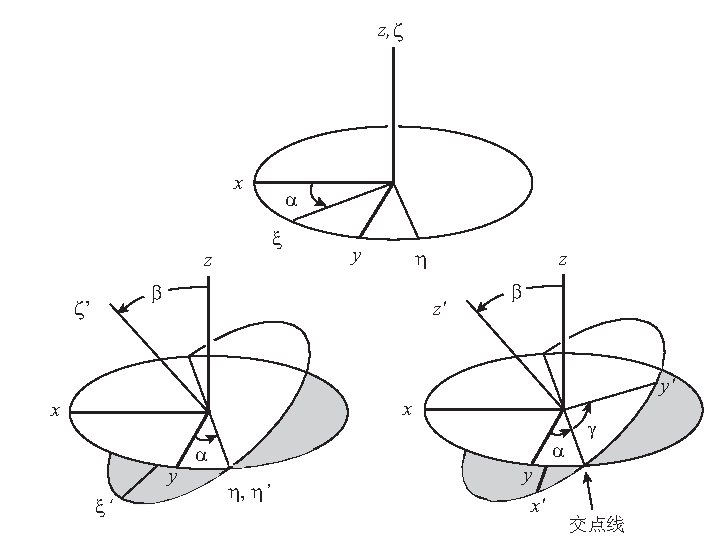
\includegraphics{../figures/appendixC/fig03.eps}
\end{center}
\caption[Euler angles]{\label{C.fig.Euler}
定义三个欧拉角的有序轴向旋转:
({\em 上图\/}) 围绕$z$轴转动角度$\alpha$的旋转${\sf A}$;
({\em 左下图\/}) 围绕交点线$\eta$转动角度$\beta$的旋转${\sf B}$;
({\em 右下图\/}) 围绕$\zeta'$轴转过角度$\gamma$的旋转${\sf C}$。
点$\bf r$的坐标从$x,y,z$变换为$x',y',z'$。}
\end{figure}
将给出的矩阵相乘,我们得到
\eqa \lefteqn{
\ssR=\!\left(\hspace{-2.0 mm}\begin{array}{ccc}
\scriptstyle{\cos\alpha\cos\beta\cos\gamma-\sin\alpha\sin\gamma} &
\scriptstyle{\sin\alpha\cos\beta\cos\gamma+\cos\alpha\sin\gamma} &
\hspace{-2.0 mm}\scriptstyle{-\sin\beta\cos\gamma} \\
\scriptstyle{-\cos\alpha\cos\beta\sin\gamma-\sin\alpha\cos\gamma} &
\scriptstyle{-\sin\alpha\cos\beta\sin\gamma+\cos\alpha\cos\gamma} &
\scriptstyle{\sin\beta\sin\gamma} \\
\scriptstyle{\cos\alpha\sin\beta} &
\scriptstyle{\sin\alpha\sin\beta} &
\scriptstyle{\cos\beta}\end{array}\hspace{-1.0 mm}\right).} \nonumber \\
&&\mbox{}
\ena
相应的有限旋转算子~(\ref{C.Dtotdef})为
\eq \label{C.DCBAdef}
\sD=\sD_C\sD_B\sD_A
=\exp(i\gamma J_z)\,\exp(i\beta J_y)\,\exp(i\alpha J_z).
\en
很容易证明,图~\ref{C.fig.Euler}的最终架构也可以由另一组有序的旋转得到:
\begin{enumerate}
\item 围绕$z$轴旋转角度\textcolor{red}{$0\leq\alpha\leq 2\pi$}。
\item 围绕{\em 原始的\/}$y$轴旋转角度$0\leq\beta\leq\pi$。
\item 围绕{\em 原始的\/}$z$轴旋转角度\textcolor{red}{$0\leq\gamma\leq 2\pi$}。
\end{enumerate}
在下面的讨论中,我们将遵照图中所示的状况,即每个后续旋转$1\rightarrow 2\rightarrow 3$都是围绕已经被旋转过的轴而进行。(\ref{C.DCBAdef})式中的操作顺序当然也必须遵守。
(A.54)和(C.238)两式之间的符号差异反映了后者的被动特性。
\index{Euler angles|)}%

%\subsection{Rotation of a generalized spherical harmonic}
\subsection{广义球谐函数的旋转}
\index{generalized spherical harmonics!rotation of|(}%
\index{spherical harmonics!generalized!rotation of|(}%

令$\bY_{lm}^N(\theta,\phi)$为单位球面$\Omega$上的广义球谐函数,且
\eq
{\bY'}_{lm}^{\raise-.4ex\hbox{$\scriptstyle{N}$}}(\theta,\phi)=
\sD\bY_{lm}^N(\theta,\phi)=\sD_C\sD_B\sD_A\bY_{lm}^N(\theta,\phi)
\en
为其旋转的等价形式。根据定义,${\bY'}_{lm}^{\raise-.4ex\hbox{$\scriptstyle{N}$}}
(\theta',\phi')=\bY_{lm}^N(\theta,\phi)$,其中$\theta',\phi'$和$\theta,\phi$ 是同一点在带撇和不带撇坐标系中的表示。
要得到旋转的张量场${\bY'}_{lm}^{\raise-.4ex\hbox{$\scriptstyle{N}$}}
(\theta,\phi)$,我们必须确定算子三重积~(\ref{C.DCBAdef}) 
作用于$\bY_{lm}^N(\theta,\phi)$的结果。由于每个广义球谐函数都是总角动量的$z$分
量的本征函数,即$J_z\bY_{lm}^N=m\bY_{lm}^N$,因此最右边算子$\sD_A=\exp(i\alpha J_z)$的作用结果为
\eqa \label{C.DofAY} \lefteqn{
\exp(i\alpha J_z)\bY_{lm}^N=
(1+i\alpha J_z-\half\alpha^2 J_z^2+\cdots)\,
\bY_{lm}^N} \nonumber \\
&&\mbox{}\hspace{14.9 mm}=
(1+im\alpha-\half m^2\alpha^2+\cdots)\bY_{lm}^N \nonumber \\
&&\mbox{}\hspace{14.9 mm}=e^{im\alpha}\,\bY_{lm}^N.
\ena
要确定交点旋转$\sD_B=\exp(i\beta J_y)$的作用,我们将其相应的生成算子写为$J_y=\half i(J_--J_+)$的形式,
并利用阶梯关系~(\ref{C.Jladfin}):
\eqa
\lefteqn{J_y\bY_{lm}^N=\half i
\sqrt{(l+m)(l-m+1)}\,\bY_{l\,m-1}^N}
\nonumber \\
&&\qquad\mbox{}-\half i\sqrt{(l-m)(l+m+1)}\,\bY_{l\,m+1}^N.
\ena
由于阶梯终止的结果,$J_y$对$\bY_{lm}^N$的重复作用总是得到具有相同次数$l$和上角标$N$的球谐函数
$\{\bY_{l\,-l}^N,\ldots,\bY_{l0}^N,\ldots,\bY_{ll}^N\}$的线性组合。
因此,$\exp(i\beta J_y)\,\bY_{lm}^N=(1+i\beta J_y-\half\beta^2 J_y^2+\cdots)\,\bY_{lm}^N$可以写成以下的形式:
\eq
\exp(i\beta J_y)\,\bY_{lm}^N=
\sum_{m'=-l}^ld_{m'm}^{(l)}(\beta)\bY_{lm'}^N,
\label{C.DofBY}
\en
其中系数$d_{m'm}^{(l)}(\beta)$待定。
最后的第三个旋转算子$\sD_C
=\exp(i\gamma J_z)$作用于~(\ref{C.DofBY})中每个球谐函数 $\bY_{lm'}^N$的结果可以通过类似于~(\ref{C.DofAY})中的推论得到:
\eq \label{C.DofCY}
\exp(i\gamma J_z)\,\bY_{lm'}^N=e^{im'\gamma}\,\bY_{lm'}^N.
\en
综合上述结果,我们得到完全旋转后的球谐函数:
\eq
{\bY'}_{lm}^{\raise-.4ex\hbox{$\scriptstyle{N}$}}=
\sum_{m'=-l}^l\sD_{m'm}^{(l)}(\alpha,\beta,\gamma)\bY_{lm'}^N,
\label{eq:bas}
\en
其中
\eq \label{C.Dmatel}
\sD_{m'm}^{(l)}(\alpha,\beta,\gamma)=e^{im'\gamma}\,d_{m'm}^{(l)}(\beta)
\,e^{im\alpha}.
\en
我们可以将~(\ref{C.Dmatel})中的量视为一个$(2l+1)\times (2l+1)$变换矩阵的分量:
\eq \label{C.Dmatel2}
\sD_{m'm}^{(l)}(\alpha,\beta,\gamma)=
\langle\bY_{lm'}^N,{\bY'}_{lm}^{\raise-.4ex\hbox{$\scriptstyle{N}$}}\rangle=
\langle\bY_{lm'}^N,\sD\bY_{lm}^N\rangle.
\en
$\sD_{m'm}^{(l)}(\alpha,\beta,\gamma)$的内积表达式~(\ref{C.Dmatel2}) 可以从~(\ref{eq:bas})式和张量正交归一关系~(\ref{C.YlmNnorm})得到。

我们现在来确定交点矩阵分量
\eq \label{C.dmatel}
d^{(l)}_{m'm}(\beta)=\langle\bY_{lm'}^N,\sD_B\bY_{lm}^N\rangle.
\en
当围绕$\byh$轴旋转角度$\{0,\beta,0\}$时,
带撇和不带撇座标之间的关系为$\theta'=\theta-\beta$、$\phi'=\phi$。
广义球谐函数 $\bY_{lm}^N$在{\em 本初子午线上\/}一点$\theta=\beta+\beta'$、$\phi=0$的值可以用
${\bY}_{l\,-l}^N,\ldots,\bY_{l0}^N,\ldots,\bY_{ll}^N$在(同一)点$\theta'=\beta'$、$\phi'=0$的值表示为
\eqa
\lefteqn{\bY_{lm}^N(\theta=\beta+\beta',\phi=0)=
{\bY'}_{lm}^{\raise-.4ex\hbox{$\scriptstyle{N}$}}(\theta'
=\beta',\phi'=0)} \label{eq:relB} \nonumber \\
&&\mbox{}=\sum_{m'=-l}^ld_{m'm}^{(l)}(\beta)
{\bY}_{lm'}^{N}(\theta'=\beta',\phi'=0).
\ena
在直觉上很明显,围绕$\byh$轴的旋转不会影响本初子午线上的球极单位矢量$\brh$、 $\bthetah$、$\bphih$;这一点可以通过在~(\ref{C.needfin})中令$\phi=0$来验证。
子午线基矢量$\beh_-$、$\beh_0$、$\beh_+$同样不受影响;
因此,我们可以用广义勒让德函数~(\ref{eq:polyno})来将~(\ref{eq:relB})写成以下形式
\eq
P_{lm}^N[\cos(\beta+\beta')]=
\sum_{m'=-l}^ld_{m'm}^{(l)}(\beta)
P_{lm'}^N(\cos\beta'). \label{eq:rltn}
\en
取$\beta'\rightarrow 0$的极限,并利用归一化关系~(\ref{C.PlmNof1}), 我们得到一个简单结果
\eq \label{C.dsupldef}
d_{m'm}^{(l)}(\beta)=P_{lm}^{m'}(\cos\beta).
\en
(\ref{C.dsupldef})式对正向旋转$0\leq\beta\leq\pi$ 是成立的。将其代回原式,我们可以将~(\ref{eq:rltn})写为矩阵分量的关系式:
\eq \label{C.d2rots}
d^{(l)}_{m'm}(\beta+\beta')=
\sum_{m''=-l}^ld_{m'm''}^{(l)}(\beta')
\,d^{(l)}_{m''m}(\beta).
\en
该式将先旋转$\beta$角接着再旋转$\beta'$角的总的旋转结果用两部分旋转的单独作用来表示。

%\subsection{Properties of the matrix elements}
\subsection{矩阵分量的性质}

有限旋转$\{\alpha,\beta,\gamma\}$的\em 逆\/}是 $\{-\gamma,-\beta,-\alpha\}$;第~\ref{C.sec.Euler}节中的每个轴向旋转都必须以相反的顺序加以“解除”。
描述此逆旋转的矩阵是转置矩阵$\ssR^{-1}=\ssR^{\rm T}=\ssA^{\rm T}\ssB^{\rm T}\ssC^{\rm T}$,
且相应的旋转算子是伴随算子
\eqa \lefteqn{
\sD^{-1}=\sD^{\dagger}
=\sD_A^{\dagger}\sD_B^{\dagger}\sD_C^{\dagger}} \nonumber \\
&&\hspace{0.88cm}\mbox{}=\exp(-i\alpha J_z)\,\exp(-i\beta J_y)\,\exp(-i\gamma J_z).
\ena
类似于~(\ref{C.Dmatel2})的矩阵分量为
\eqa \label{C.Dmatel3} \lefteqn{
\sD_{m'm}^{(l)}(-\gamma,\,-\beta,\,-\alpha)=
\langle\bY_{lm'}^N,\sD^{\dagger}\bY_{lm}^N\rangle
=\langle\sD\bY_{lm'}^N,\bY_{lm}^N\rangle} \nonumber \\
&&\mbox{}=\langle\bY_{lm}^N,\sD\bY_{lm'}^N\rangle^*
=\sD^{(l)*}_{mm'}(\alpha,\beta,\gamma).
\ena
令$\alpha=\gamma=0$,并注意到 $d^{(l)}_{mm'}(\beta)$为实数,我们发现特别的一点是
\eq \label{C.dsupldef2}
d^{(l)}_{m'm}(-\beta)=d^{(l)}_{mm'}(\beta).
\en
(\ref{C.Dmatel3})和~(\ref{C.dsupldef2})定义了欧拉角为负值$-2\pi\leq\alpha<0$, $-\pi\leq\beta<0$、$-2\pi\leq\gamma<0$
的$\sD_{m'm}^{(l)}(\alpha,\beta,\gamma)$和$d^{(l)}_{m'm}(\beta)$。

旋转后的球谐函数的正交归一性确保了
\eq
\langle\sD\bY_{lm}^N,\sD\bY_{lm'}^N\rangle
=\langle\bY_{lm}^N,\sD^{\dagger}\sD\bY_{lm'}^N\rangle
=\delta_{mm'}
\en
或者等价的
\eq \label{C.Dunitary}
\sum_{m''=-l}^l\sD^{(l)*}_{m''m}(\alpha,\beta,\gamma)\,
\sD^{(l)}_{m''m'}(\alpha,\beta,\gamma)=\delta_{mm'}.
\en
在上式中令$\alpha=\gamma=0$,或者在(\ref{C.d2rots})中令$\beta'=-\beta$并利用~(\ref{C.dsupldef2}),我们得到
\eq \label{C.dunitary}
\sum_{m''=-l}^ld^{(l)}_{m''m}(\beta)\,
d^{(l)}_{m''m'}(\beta)=\delta_{mm'}.
\en
(\ref{C.Dunitary})--(\ref{C.dunitary})规定了
$(2l+1)\times (2l+1)$矩阵~(\ref{C.Dmatel2})--(\ref{C.dmatel})
是{\em unitar幺正的\/}。在(\ref{C.dunitary})辨识出~(C.255),便可得到~(C.127)这一结果。

从~(\ref{C.PlmNsymm})中给出的广义勒让德函数$P_{lm}^{m'}(\cos\beta)$的对称关系,可以立刻得到$d^{(l)}_{m'm}(\beta)$所满足的对称关系。
例如,对于一个固定旋转$\beta$,我们有
\eq \label{C.dsymm}
d^{(l)}_{-m'\,-m}(\beta)=(-1)^{m+m'}d^{(l)}_{m'm}(\beta),
\en
\eq
d^{(l)}_{mm'}(\beta)=(-1)^{m+m'}d^{(l)}_{m'm}(\beta),
\en
\eq \label{C.dsymm3}
d^{(l)}_{-m\,-m'}(\beta)=d^{(l)}_{m'm}(\beta).
\en
我们可以轻而易举地将~(\ref{C.dsymm})--(\ref{C.dsymm3})扩展到完整的矩阵分量;
尤其是,我们发现~(\ref{C.Dmatel})的复数共轭为
\eq \label{C.Dstar}
\sD^{(l)*}_{m'm}(\alpha,\beta,\gamma)=(-1)^{m'+m}
\,\sD^{(l)}_{-m'\,-m}(\alpha,\beta,\gamma).
\en
(\ref{C.3jdef5})--(\ref{C.3jdef6}) 也可以用同样的方式扩展,而得到等价的矩阵分量关系
\eqa \label{C.drel1}
\lefteqn{\sD^{(l_1)}_{m_1^{\prime}m_1}
\sD^{(l_2)}_{m_2^{\prime}m_2}=
\sum_l\sum_{m'}\sum_m\,(2l+1)
\left(\begin{array}{ccc}
l & l_1 & l_2 \\ m' & m_1^{\prime} & m_2^{\prime}
\end{array}\right)} \nonumber \\
&&\mbox{}\times\left(\begin{array}{ccc}
l & l_1 & l_2 \\ m & m_1 & m_2
\end{array}\right)\sD^{(l)*}_{m'm},
\ena
\eqa \label{C.drel2}
\lefteqn{(2l+1)^{-1}\,\delta_{ll'}\,\sD^{(l)*}_{m'm}=
\sum_{m_1^{\prime}m_2^{\prime}}\,\sum_{m_1m_2}
\left(\begin{array}{ccc}
l & l_1 & l_2 \\ m' & m_1^{\prime} & m_2^{\prime}
\end{array}\right)} \nonumber \\
&&\mbox{}\times\left(\begin{array}{ccc}
l' & l_1 & l_2 \\ m & m_1 & m_2
\end{array}\right)
\sD^{(l_1)}_{m_1^{\prime}m_1}
\sD^{(l_2)}_{m_2^{\prime}m_2},
\ena
其中略去了相同的自变量$\alpha,\beta,\gamma$。
利用变换矩阵~(\ref{C.Dunitary})的幺正特性,我们得到完全对称的关系:
\eqa \label{C.drel3}
\lefteqn{\sum_{m'}\sum_{m_1^{\prime}}\sum_{m_2^{\prime}}
\,\sD^{(l)}_{m'm}\sD^{(l_1)}_{m_1^{\prime}m_1}
\sD^{(l_2)}_{m_2^{\prime}m_2}
\left(\begin{array}{ccc}
l & l_1 & l_2 \\ m' & m_1^{\prime} & m_2^{\prime}
\end{array}\right)} \nonumber \\
&&\mbox{}=\left(\begin{array}{ccc}
l & l_1 & l_2 \\ m & m_1 & m_2
\end{array}\right).
\ena
若有需要,该式可以进一步转化为类似的包含广义勒让德函数的对称关系式。

完整矩阵的分量对三个欧拉角$\{\alpha,\beta,\gamma\}$的积分是正交归一的,即
\eqa \label{C.drel5} \lefteqn{
\frac{1}{8\pi^2}\int_0^{2\pi}\int_0^{\pi}\int_0^{2\pi}
\sD^{(l_1)*}_{m_1^{\prime}m_1}\sD^{(l_2)}_{m_2^{\prime}m_2}
\,d\/\alpha\hspace{0.3 mm}\sin\beta\,d\/\beta\,d\/\gamma} \nonumber \\
&&\mbox{}=(2l_1+1)^{-1}
\delta_{l_1l_2}
\textcolor{red}{\delta_{m_1m_2}\delta_{m_1^{\prime}m_2^{\prime}}}
\ena
利用~(\ref{C.3jdef4})可以得到三个矩阵分量的积分
\eqa \label{C.drel6} \lefteqn{
\frac{1}{8\pi^2}\int_0^{2\pi}\int_0^{\pi}\int_0^{2\pi}\sD^{(l)}_{m'm}
\sD^{(l_1)}_{m_1^{\prime}m_1}\sD^{(l_2)}_{m_2^{\prime}m_2}
\,d\/\alpha\hspace{0.3 mm}\sin\beta\,d\/\beta\,d\/\gamma} \nonumber \\
&&\mbox{}=\left(\begin{array}{ccc}
l & l_1 & l_2 \\ m' & m_1^{\prime} & m_2^{\prime}
\end{array}\right)\left(\begin{array}{ccc}
l & l_1 & l_2 \\ m & m_1 & m_2
\end{array}\right).
\ena
很明显,利用对称性~(\ref{C.Dstar})把~(\ref{C.drel6})中的第一个分量变为复数共轭,便可以将其改写为类似于~(\ref{C.3jdef2})的形式。而 $1/8\pi^2$这一因子则可被认为是角积分的总"体积"。
\index{generalized spherical harmonics!rotation of|)}%
\index{spherical harmonics!generalized!rotation of|)}%

%\subsection{Addition theorem}
\subsection{加法定理}
\label{C.sec.addth}
\index{addition theorem|(}%
\index{spherical-harmonic addition theorem|(}%
\index{spherical harmonics!addition theorem|(}%
\index{generalized spherical harmonics!addition theorem|(}%

$\ssR_1=\{\alpha_1,\beta_1,\gamma_1\}$在先$\ssR_2=\{\alpha_2,\beta_2,\gamma_2\}$随后的两个接续旋转的净结果是一个{\em 单一\/}旋转 $\ssR=\ssR_2\ssR_1=\{\alpha,\beta,\gamma\}$,
其欧拉角为
\eq \label{C.2rots1}
\cos(\alpha-\alpha_1)=\frac{\cos\beta_2-\cos\beta\cos\beta_1}
{\sin\beta\sin\beta_1},
\en
\eq \label{C.2rots2}
\cos\beta=\cos\beta_1\cos\beta_2-\sin\beta_1\sin\beta_2\cos(\alpha_2+\gamma_1),
\en
\eq \label{C.2rots3}
\cos(\gamma-\gamma_2)=\frac{\cos\beta_1-\cos\beta\cos\beta_2}
{\sin\beta\sin\beta_2}.
\en
与这些旋转相应的算子满足$\sD(\ssR)=\sD(\ssR_2)\sD(\ssR_1)$,或等价的
\eq \label{C.addth2}
\sD_{m'm}^{(l)}(\alpha,\beta,\gamma)=\sum_{m''=-l}^l
\sD_{m'm''}^{(l)}(\alpha_2,\beta_2,\gamma_2)
\,\sD_{m''m}^{(l)}(\alpha_1,\beta_1,\gamma_1).
\en
矩阵分量关系~(\ref{C.addth2})是所谓的{\em 加法定理\/}的最一般的形式。
当$\{\alpha_1,\beta_1,\gamma_1\}=\{0,\beta,0\}$
和$\{\alpha_2,\beta_2,\gamma_2\}=\{0,\beta',0\}$时,它简化为单轴结果~(\ref{C.d2rots}),而当第二个旋转为第一个的逆($\{\alpha_2,\beta_2,\gamma_2\}=
\{-\gamma_1,-\beta_1,-\alpha_1\}$)时,则简化成幺正关系式~(\ref{C.Dunitary})。

对(\ref{C.addth2})式中的欧拉角做其它选择会产生一些不同的专门化的加法定理;例如,如果设定$m'=m=0$、$\{\alpha_1,\beta_1,\gamma_1\}=\{0,\theta_1,\phi_1\}$以及
$\{\alpha_2,\beta_2,\gamma_2\}=\{\pi-\phi_2,\theta_2,0\}$,我们得到
\eq
\left(\frac{2l+1}{4\pi}\right)P_l(\cos\Theta)=
\sum_{m=-l}^lY_{lm}^*(\theta_2,\phi_2)Y^{}_{lm}(\theta_1,\phi_1),
\label{eq:addylm}
\en
其中$\cos\Theta=\cos\theta_2\cos\theta_1+\sin\theta_2\sin\theta_1
\cos(\phi_2-\phi_1)$。这一结果是经典的球谐函数加法定理(\ref{B.addtheor}),它的推导也可以用更简单的方式,通过计算如下旋转不变量表达式的左边
\eq
\sum_{m=-l}^l{Y'}_{lm}^*(\theta_2',\phi_2'){Y'}_{lm}(\theta_1',\phi_1')=
\sum_{m=-l}^lY_{lm}^*(\theta_2,\phi_2)Y^{}_{lm}(\theta_1,\phi_1)
\en
在旋转后的点$\theta_1',\phi_1'$或$\theta_2',\phi_2'$趋于北极或南极的极限时而得到。
\index{addition theorem|)}%
\index{spherical-harmonic addition theorem|)}%
\index{spherical harmonics!addition theorem|)}%
\index{generalized spherical harmonics!addition theorem|)}%

%\subsection{Recursion relations}
\subsection{递推关系}

矩阵分量$d^{(l)}_{m'm}(\beta)$ 可以利用广义勒让德函数满足的递推关系式~(\ref{C.mrecur})--(\ref{C.Nrecur})来计算。
我们可以用固定$m'$的关系式
\eqa \label{C.mrecur2}
\lefteqn{\left[m'(\sin\beta)^{-1}-m\cot\beta\right]d^{(l)}_{m'm}
=\half\sqrt{(l+m)(l-m+1)}\,d^{(l)}_{m'\,m-1}} \nonumber \\
&&\mbox{}+\half\sqrt{(l-m)(l+m+1)}\,d^{(l)}_{m'\,m+1}
\ena
分别从$m=\pm l$向下和向上迭代,在$m=m'\cos\beta$处汇合;或者用固定$m$的关系式
\eqa \label{C.mprecur}
\lefteqn{\left[m'\cot\beta-m(\sin\beta)^{-1}\right]d^{(l)}_{m'm}
=\half\sqrt{(l+m')(l-m'+1)}\,d^{(l)}_{m'-1\,m}} \nonumber \\
&&\mbox{}+\half\sqrt{(l-m')(l+m'+1)}\,d^{(l)}_{m'+1\,m}
\ena
分别从$m'=\pm l$向下和向上迭代,在$m'=m(\cos\beta)^{-1}$处汇合。
还有其它的计算方案,例如,Edmonds (\citeyear{edmonds60}) 
展示了如何用雅可比多项式来表示分量$d^{(l)}_{m'm}(\beta)$,该多项式可以用另一种递推关系来计算。

%\subsection{Rotation of an arbitrary tensor}
\subsection{任意张量的旋转}

最后,我们考虑有限旋转 $\{\alpha,\beta,\gamma\}$作用于以广义球谐函数表示的任意张量场
\eq \label{C.Tunrot}
\bT=\sum_{l=0}^\infty\sum_{m=-l}^l
T_{lm}^{\alpha_1\cdots\alpha_n}\bY_{lm}^N.
\en
的结果。用(\ref{eq:bas})式可以得到旋转后的场为
\eqa \label{C.Ttransf1} \lefteqn{
\bT'=\sD\bT=\sum_{l=0}^\infty\sum_{m=-l}^l
T_{lm}^{\alpha_1\cdots\alpha_n}\left(\sD\bY_{lm}^N\right)} \nonumber \\
&&\mbox{}\hspace{7.0 mm}=\sum_{l=0}^\infty\sum_{m=-l}^l\sum_{m'=-l}^l
\sD_{m'm}^{(l)}(\alpha,\beta,\gamma)\,
T_{lm}^{\alpha_1\cdots\alpha_n}\bY_{lm'}^N.
\ena
我们可以将~(\ref{C.Ttransf1})这一结果改写为类似于~(\ref{C.Tunrot})的形式:
\eq
\bT'=\sum_{l=0}^\infty\sum_{m=-l}^l
T_{lm}^{\prime\alpha_1\cdots\alpha_q}\bY_{lm}^N.
\label{eq:relati}
\en
{\em 变换后的展开系数\/}$T_{lm}^{\prime\alpha_1\cdots\alpha_q}$与原来的系数 $T_{lm}^{\alpha_1\cdots\alpha_q}$之间有以下关系
\eq
T_{lm}^{\prime\alpha_1\cdots\alpha_q}
=\sum_{m'=-l}^l\sD_{mm'}^{(l)}(\alpha,\beta,\gamma)\,
T_{lm'}^{\alpha_1\cdots\alpha_q}.
\label{eq:expan}
\en
要注意从基的变换关系式~(\ref{eq:bas})到~(\ref{eq:expan})式的“角标的误导”;
变换后的系数$T_{lm}^{\prime\alpha_1\cdots\alpha_q}$ 是用类似于~(\ref{A.ueqTv})式的方式以{\em 普通矩阵相乘\/}来计算的。
用幺正性质~(\ref{C.Dunitary})可以得到(\ref{eq:expan})的逆为
\eq
T_{lm}^{\alpha_1\cdots\alpha_q}
=\sum_{m'=-l}^l\sD_{m'm}^{(l)*}(\alpha,\beta,\gamma)\,
T_{lm'}^{\prime\alpha_1\cdots\alpha_q}.
\label{eq:expan2}
\en
旋转后和原来的偏导数$\p/\p T_{lm}^{\prime\alpha_1\cdots\alpha_n}$和$\p/\p T_{lm}^{\alpha_1\cdots\alpha_q}$之间的关系为
\eq \label{C.partT}
\p/\p T_{lm}^{\prime\alpha_1\cdots\alpha_q}
=\sum_{m'=-l}^l\sD_{mm'}^{(l)*}(\alpha,\beta,\gamma)\,
(\p/\p T_{lm'}^{\alpha_1\cdots\alpha_q})
\en
和
\eq \label{C.partT2}
\p/\p T_{lm}^{\alpha_1\cdots\alpha_q}
=\sum_{m'=-l}^l\sD_{m'm}^{(l)}(\alpha,\beta,\gamma)\,
(\p/\p T_{lm'}^{\prime\alpha_1\cdots\alpha_q}).
\en
变换关系~(\ref{C.partT})和~(\ref{C.partT2})在涉及张量场$\bT$和 $\bT'=\sD\bT$的反问题中是很有用的。

%\subsection{Rotation to the equator}
\subsection{旋转至赤道}
\index{rotation to the equator|(}%
\label{section:C.8.7}

在本附录的最后,我们考虑将一个“源点”$\theta_1,\phi_1$和一个“接收点”$\theta_2,\phi_2$ 旋转至赤道的问题。
我们要求旋转后的源点位于本初子午线上,因而
\eq \label{C.eqrot}
\theta_1^{\prime}=\pi/2,\;\phi_1^{\prime}=0\quad
\mbox{and}\quad\theta_2^{\prime}=\pi/2,\;
\phi_2^{\prime}=\Theta,
\en
其中$\Theta$为两点之间的测地角距离,由$\cos\Theta=\cos\theta_2\cos\theta_1
+\sin\theta_2\sin\theta_1\cos(\phi_2-\phi_1)$给定。
实现变换~(\ref{C.eqrot})的欧拉角$\{\alpha,\beta,\gamma\}$为
\eq
\label{C.poledef1}
\tan\alpha=\frac{\sin\theta_2\cos\theta_1\cos\phi_2
-\cos\theta_2\sin\theta_1\cos\phi_1}
{\cos\theta_2\sin\theta_1\sin\phi_1
-\sin\theta_2\cos\theta_1\sin\phi_2},
\en
\eq \label{C.poledef2}
\cos\beta=\frac{\sin\theta_2\sin\theta_1\sin(\phi_2-\phi_1)}
{\sin\Theta},
\en
\eq \label{C.poledef3}
\tan\gamma=\frac{\cos\theta_1\cos\Theta-\cos\theta_2}
{\cos\theta_1\sin\Theta}.
\en
对比~(\ref{C.poledef1})--(\ref{C.poledef2})
和~(\ref{B.poledef1})--(\ref{B.poledef2}),我们认出
\eq \label{C.first2rots}
\alpha=\bar{\phi},\qquad\beta=\bar{\theta}.
\en
前两个旋转~(\ref{C.first2rots})将$\bzh$轴转到源点-接收点大圆的正的极点 $\bar{\theta},\bar{\phi}$,
而第三个旋转则将本初子午线沿着新的赤道转到源点。
图~\ref{C.fig.RioCairo}展示了变换~(\ref{C.eqrot});
这个例子中,测地劣弧的两个端点$\theta_1,\phi_1$和$\theta_2,\phi_2$ 分别位于里约热内卢和开罗。
\begin{figure}
\begin{center}
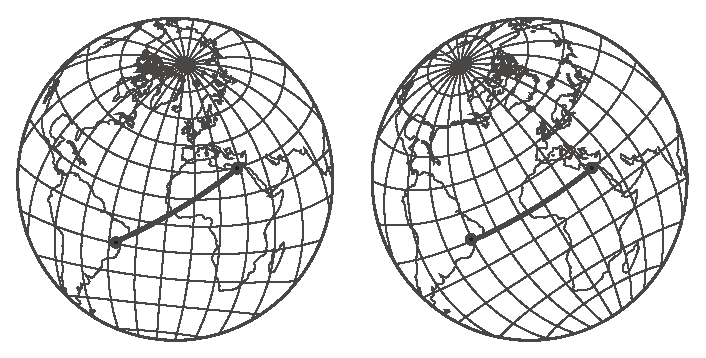
\includegraphics{../figures/appendixC/fig04.eps}
\end{center}
\caption[Rio to Cairo]{\label{C.fig.RioCairo}
里约热内卢到开罗的劣弧路径的被动旋转。
({\em 左图\/})粗线大圆弧表示原来的路径。
({\em 右图\/})在新的带撇坐标系中,里约热内卢位于赤道和本初子午线的交点:$\theta_1^{\prime}=\pi/2,
\,\phi_1^{\prime}=0$。开罗也在赤道上,在东方$\Theta\approx 90^{\circ}$处:
$\theta_2^{\prime}=\pi/2,\,\phi_2^{\prime}=\Theta$.}
\end{figure}
要注意旋转的被动性:球面上的海岸线与其它特征的位置$\brh$ 保持不变,但是带撇和不带撇的坐标线却有所不同。

除了其它用途之外,将$\theta_1,\phi_1$和$\theta_2,\phi_2$旋转到赤道上的这一结果 还可以用来计算标量场$\psi$在源点和接收点之间测地路径上的积分:
\eq \label{C.pathint}
\int_{\theta_1,\phi_1}^{\theta_2,\phi_2}\psi(\theta,\phi)
\,d\/\Delta=\sum_{l=0}^{\infty}\sum_{m=-l}^l\psi_{lm}
\int_{\theta_1,\phi_1}^{\theta_2,\phi_2}
Y_{lm}(\theta,\phi)\,d\/\Delta.
\en
如我们在第~\ref{16.sec.eqrot}节中所讨论的,当费马原理应用于面波层析成像时会出现 形如~(\ref{C.pathint})的路径积分;
在这种情况下,场$\psi$是单频勒夫或瑞利波的相速度的倒数。
复数表面球谐函数$Y_{lm}$的积分为
\eqa \label{C.pathint2} \lefteqn{
\int_{\theta_1,\phi_1}^{\theta_2,\phi_2}
Y_{lm}(\theta,\phi)\,d\/\Delta=
\int_0^{\Theta}Y_{lm}^{\prime}(\pi/2,\phi')\,d\/\phi'}
\nonumber \\
&&\mbox{}=\sum_{m'=-l}^l(i/m')\,X_{lm'}(\pi/2)
\,(1-e^{im'\Theta})\,\sD^{(l)}_{m'm}
(\alpha,\beta,\gamma),
\ena
其中我们借助了~(\ref{eq:bas}),并将积分$\int_0^{\Theta}
e^{im\phi'}\,d\/\phi'$进行了解析计算。
将~(\ref{C.pathint2})代入~(\ref{C.pathint}),我们发现
\eqa \label{C.pathint3} \lefteqn{
\int_{\theta_1,\phi_1}^{\theta_2,\phi_2}
\psi(\theta,\phi)\,d\/\Delta=
\sum_{l=0}^{\infty}\sum_{m=-l}^l
(i/m)\,X_{lm}(\pi/2)\,(1-e^{im\Theta})} \nonumber \\
&&\mbox{}\times\sum_{m'=-l}^l\sD^{(l)}_{mm'}
(\alpha,\beta,\gamma)\,\psi_{lm}.
\ena
这里我们互换了角标$m$和$m'$,
目的是为了明确~(\ref{C.pathint3})中最后一个求和仅仅是变换后的展开系数${\psi}_{lm}^{\prime}$。
利用简单关系式~(\ref{B.Psipsi}),可以很容易地将实数场$\psi$的积分用实数的展开系数 $\Psi_{lm}$或$a_{l0},a_{lm},b_{lm}$来表示。

在$\Theta\rightarrow2\pi$极限下,(\ref{C.pathint2})式中的量$(i/m')(1-e^{im'\Theta})$简化为$2\pi\hspace{0.3 mm}\delta_{m'0}$。
因此,在一个完整的大圆路径$\bar{\theta},\bar{\phi}$上,球谐函数$Y_{lm}$的平均值为
\eq \label{C.pathint4}
\frac{1}{2\pi}\oint_{\,\bar{\theta},\bar{\phi}}
Y_{lm}(\theta,\phi)
\,d\/\Delta=P_l(0)Y_{lm}(\bar{\theta},\bar{\phi}).
\en
任一场的大圆平均的展开系数$\bar{\psi}_{lm}$ 
与原来的系数$\psi_{lm}$之间的关系为$\bar{\psi}_{lm}=P_l(0)\,\psi_{lm}$。
一如预期的,这些结果与~(\ref{B.Ylmoint})--(\ref{B.psibarlm})是一致的。
\index{rotation to the equator|)}%
\index{tensor field!rotation of|)}%
